% ------------------------------------------------------------------------
% ------------------------------------------------------------------------
% Tese de Mestrado da Escola Politécnica da USP
% Integrantes: Gabriel Takaoka Nishimura
% ------------------------------------------------------------------------
% ------------------------------------------------------------------------

\documentclass[
	12pt,				% tamanho da fonte
	openright,			% capítulos começam em pág ímpar
	oneside,			% para impressão em recto e verso. Oposto a 
	a4paper,			% tamanho do papel.
	hyphens,			% url longa nas referencias
	english,			% idioma adicional para hifenização
	english				% o último idioma é o principal do documento
]{abntex2}
% ---
%  PACOTES
% ---

% Pacotes básicos
\usepackage{lmodern}			% Usa a fonte Latin Modern
\usepackage[T1]{fontenc}		% Selecao de codigos de fonte.
\usepackage[utf8]{inputenc}		% Conversão automática dos acentos
\usepackage{lastpage}			% Usado pela Ficha catalográfica
\usepackage{indentfirst}		% Indenta o primeiro parágrafo de cada seção.
\usepackage{color}				% Controle das cores
\usepackage{amssymb}			% Less than or equal to
\usepackage{float}				% Gráficos
\usepackage{microtype} 			% para melhorias de justificação
\usepackage{listings}			% para listagem de código %
\usepackage{amsmath}			% para construção de sistemas lineares%
\usepackage{graphicx}
\usepackage{pgfplots}
\usepackage{lscape}
\usepackage{longtable}
\usepackage{multirow}
\usepackage{caption}
\usepackage{subcaption}
\usepackage{threeparttable}
\usepackage{libs/tikz-uml}
\usepackage{makecell}

\graphicspath{ {images/} }

% Pacotes de citações
\usepackage[brazilian,hyperpageref]{backref}	 % Paginas com as citações
\usepackage[alf,num,abnt-url-package=url]{abntex2cite}	% Citações padrão ABNT

\pgfplotsset{compat=1.17}
% ---
% CONFIGURAÇÕES DE PACOTES
% ---

% LISTING CAPTION POST
\lstset{
  basicstyle=\ttfamily,
  columns=fullflexible,
  breaklines=true,
  inputencoding=utf8,
  extendedchars=true,
  literate={á}{{\'a}}1 {ã}{{\~a}}1 {é}{{\'e}}1,
}

\makeatletter

\lst@Key{source}{}{\def\lst@source{#1}}

\let\orig@lst@MakeCaption=\lst@MakeCaption
\def\lst@MakeCaption#1{%
    \orig@lst@MakeCaption#1%
    \ifx b#1%
        \ifx\lst@source\@empty\else
            \noindent
            \expandafter\lst@makesourcebox\expandafter{\lst@source}%
            \vskip\belowcaptionskip
        \fi
    \fi
}

\def\lst@makesourcebox#1{%
    \makebox[\linewidth][c]{\textrm{Source: #1}}%
}
\makeatother
\lstset{backgroundcolor=\color{lightgray}}

% ---
% Configurações do pacote
\newenvironment{spmatrix}[1]{
	\def\mysubscript{#1}\mathop\bgroup\begin{pmatrix}
	}
{\end{pmatrix}\egroup_{\textstyle\mathstrut\mysubscript}}
% ---

% ---
% Configurações do pacote float
\newfloat{chart}{tbhp}{loc} %section
\floatname{chart}{Charts}
\floatstyle{plaintop}
\restylefloat{chart}
\newcommand{\listofcharts}{\listof{chart}{Charts List}}
% ---
% Configurações do pacote backref
\renewcommand{\backrefpagesname}{Citation(s) on page(s):~}
\renewcommand{\backref}{}
\renewcommand*{\backrefalt}[4]{
	\ifcase #1 %
	No citation.%
	\or
	Cited on page #2.%
	\else
	Cited #1 times in pages #2.%
	\fi}%


% ---
% ---
% Informações de dados para CAPA e FOLHA DE ROSTO
% ---
% \titulo{Fale Alguma Coisa - a citizen science collected brazilian portuguese speech corpus}
\titulo{Fale Alguma Coisa - A Brazilian Portuguese Speech Corpus Constructed through Citizen Science and Gamification}
\autor{Gabriel Takaoka Nishimura}
\local{São Paulo}
\data{2021}
\orientador{Prof. Dr. Bruno Carvalho de Albertini}
\instituicao{São Paulo University -  USP \par
			Polytechnic School \par
			Computer Engineering with emphasys on Computer}
\tipotrabalho{Mestrado}
\preambulo{Research Proposal presented to the Polytechnic School of the University of São Paulo}
% ---

% ---
% Configurações de aparência do PDF final
\definecolor{blue}{RGB}{41,5,195} % cor azul

% informações do PDF
\makeatletter
\hypersetup{
	%pagebackref=true,
	pdftitle={\@title},
	pdfauthor={\@author},
	pdfsubject={\imprimirpreambulo},
	pdfcreator={LaTeX with abnTeX2},
	pdfkeywords={abnt}{latex}{abntex}{abntex2}{trabalho acadêmico},
	colorlinks=true,       		% false: boxed links; true: colored links
	linkcolor=blue,          	% color of internal links
	citecolor=blue,        		% color of links to bibliography
	filecolor=magenta,      	% color of file links
	urlcolor=blue,
	bookmarksdepth=4
}
\makeatother
% ---

% ---
% Espaçamentos entre linhas e parágrafos
% ---
\setlength{\parindent}{1.3cm} % O tamanho do parágrafo
\setlength{\parskip}{0.2cm}  % espacamento entre um paragrafo e outro

% ---
% compila o indice
% ---
\makeindex
% ---

% ----
% Início do documento
% ----
\begin{document}

	% Seleciona o idioma do documento
	\selectlanguage{english}

	% Retira espaço extra obsoleto entre as frases.
	\frenchspacing

	% ----------------------------------------------------------
	% ELEMENTOS PRÉ-TEXTUAIS
	% ----------------------------------------------------------
	\pretextual

	% ---
	% Capa
	% ---
	\imprimircapa
	% ---

	% ---
	% Folha de rosto
	% ---
	\imprimirfolhaderosto*
	% ---
	
    % ========== Dedicatória (opcional) ==========
    \dedicatoria{
    I dedicate this work to my long-time life partner, Vivian. You gave me the strength to press forward, even when all hope was lost and my motivation long gone. You taught me that with discipline, a good night of sleep, and a well-brewed \textit{matcha latte} I can do anything. This one is for you.
    }
    
    
    % ========== Agradecimentos ==========
    \begin{agradecimentos}
    My supervisor Bruno Carvalho de Albertini. For putting up with my confusion and despair, even managing to motivate me. With your help, I was able to overcome a lot of rough patches and properly structure this chaos. Thank you so much for your time and patience.

    Ricardo Tiburcio Humaytá, for the stupendous work done in the implementation of the user interface of the Fale Alguma Coisa app. Thanks to you, this has turned into something else. All the discussions were worth all the time! Moreover, thank you for the CSS tips, aligning and layering is hard.
    
    Daniel Noriaki Kurosawa, for directly helping me develop some of the features, namely the home and login page! Sorry for the harsh code reviews...
    
    My two awesome text reviewers, Caique Bernardes Magalhães Queiroz and Carolina Ribeiro Minchin.

    My family (including our 4 dogs), for supporting me in these trying times. Helping me in ways I could not even fathom possible.
    
    My friends, for putting up with my shenanigans. Anything that takes this amount of time is a long time, but who would have guessed?
    
    Without you all, this would not have been possible.
    \end{agradecimentos}
    
    % ========== Epígrafe (opcional) ==========
    \begin{epigrafe}
    \vspace*{\fill}
    \begin{flushright}
    {``Words are where most change begins.``} \\ Shallan Davar, Words of Radiance \\ Brandon Sanderson
    \end{flushright}
    \end{epigrafe}
        
        
	% ---
	% RESUMOS
	% ---
	% ---
% Arquivo com o resumo da Tese de Mestrado do aluno
% Gabriel Takaoka Nishimura da Escola Politécnica da Universidade de São Paulo
% ---

\setlength{\absparsep}{18pt}
\begin{resumo}
    Citizen science is a powerful tool to help scientists advancing scientific knowledge, driving many breakthroughs by the sheer volume of nonprofessional contributions. This is made possible by the advancement in technology, connectivity and interest in science by the public; but also by some techniques to engage users, namely, gamification. The addition of game elements is widely used in the private sector, however, the academic field is also able to benefit from it,
    retaining usage in crowd-sourced environments. This combination allows for citizen science to employ labor in tasks not suitable for automation, such as data gathering or classification, whilst allowing a fun and engaging experience. Many research fields in Computer Science highly depend on this kind of human generated data, with requirements on quantity and quality. This research focuses on Natural Language Processing, as it also has such data intensive requirements, more specifically voice recognition. Many approaches to train systems in voice recognition require voice datasets, or speech corpora, with multiple hours of voice recording and transcriptions. This work identifies citizen science gamified approaches as an opportunity to create such a dataset. Therefore, a gamified voice recording web application is conceptualized, developed, and deployed to accept user contributions. After a submission period, data acquired is validated and filtered, generating a speech corpus. This dataset is made publicly available through the CC-BY open-source license.
	\vspace{\onelineskip}
	\noindent 
	
	\textbf{Key-words}: citizen science, gamification, speech corpus, natural language processing
\end{resumo}

	% ---

	% ---
	% inserir lista de ilustrações
	% ---
	\pdfbookmark[0]{\listfigurename}{lof}
	\listoffigures*
	\cleardoublepage
	% ---

	% ---
	% inserir lista de gráficos
	% ---
	% \pdfbookmark[0]{\listtablename}{lot}
	% \listofcharts
	% \cleardoublepage
	% ---

	% ---
	% inserir lista de tabelas
	% ---
	\pdfbookmark[0]{\listtablename}{lot}
	\listoftables*
	\cleardoublepage
	% ---

	% ---
	% inserir lista de abreviaturas e siglas
	% ---
	
	% ---
	
	% ---
	% code listing
	% ---
	
    \lstlistoflistings
    \clearpage

	% ---
	% inserir o sumario
	% ---
	\pdfbookmark[0]{\contentsname}{toc}
	\tableofcontents*
	\cleardoublepage
	% ---

	% ----------------------------------------------------------
	% ELEMENTOS TEXTUAIS
	% ----------------------------------------------------------
	\textual

	% ----------------------------------------------------------
	% Introdução
	% ----------------------------------------------------------
	\chapter*[Introduction]{Introduction}
\addcontentsline{toc}{chapter}{Introduction}

The research and advancement of scientific knowledge can be very daunting, especially without a scientific background. Requirements such as a well-defined methodology, high data quality, and a strict revision process may present some barriers to the common citizen. However, with the recent advancement in technology \cite{newman2012future}, connectivity \cite{newman2012future} and interest in science by the public \cite{silvertown2009new}, there has been a rising trend in the general populace contributing to a special kind of science: Citizen Science \cite{mckinley2017citizen}.

Citizen science refers to research that engages nonprofessionals in the process of creating new scientific knowledge \cite{bonney2014next}. Referred to as citizen scientists; these nonprofessionals may participate in a variety of tasks ranging in complexity; from simple tasks such as data gathering or classification \cite{barker2013pascal}, to even complex ones such as solving algorithms \cite{cooper2010predicting}. They may act as contributors and collaborators, but can also have a more proactive role as a project leader \cite{robinson2018ten}.

Citizen science is not new, as it has existed for more than one century now. However, its reach was reduced, since it was mostly focused on ecological and environmental sciences. Some initiatives date back to 1890, such as the Cooperative Weather Service, where amateurs send collected weather data to the National Weather Service; and 1966, the North American Breeding Bird Survey with more than 670 publications referencing it, where nonprofessionals map avian species distribution throughout North America over time. This practice has shown a rise in (1) the number of citizen science projects \footnote{Extraction from \href{citizenscience.gov}{citizenscience.gov}, and Zooniverse.} (figure \ref{fig:growth-citizen-science-projects}) as well as (2) articles published on the topic \footnote{Query String: "citizen science" in Scholar Google, filtered by one year intervals} (as seen in figure \ref{fig:growth-publications}).

\pgfplotstableread[row sep=\\,col sep=&]{
    year & publications \\
    2010 & 2810 \\
    2011 & 2750 \\
    2012 & 5220 \\
    2013 & 6990 \\
    2014 & 9330 \\
    2015 & 11900 \\
    2016 & 14500 \\
    2017 & 15800 \\
    2018 & 20200 \\
    2019 & 18300 \\
}\publicationdata

\begin{figure}[!h]
    \centering
    \begin{tikzpicture}
        \begin{axis}[
                ybar,
                bar width=.5cm,
                width=\textwidth,
                height=.5\textwidth,
                legend style={at={(0, 10)}, anchor=north,legend columns=-1},
                symbolic x coords={2010,2011,2012,2013,2014,2015,2016,2017,2018,2019,2020},
                xtick=data,
                nodes near coords,
                nodes near coords align={vertical},
                ymin=0,ymax=25000,
                ylabel={publications},
                xlabel={years},
            ]
            \addplot table[x=year,y=publications]{\publicationdata};
        \end{axis}
    \end{tikzpicture}
    \caption{Growth of citizen science initiatives over time}
    \label{fig:growth-citizen-science-projects}
\end{figure}

\begin{figure}[!h]
    \centering
    \begin{tikzpicture}
        \begin{axis}[
                ybar,
                bar width=.5cm,
                width=\textwidth,
                height=.5\textwidth,
                legend style={at={(0, 10)}, anchor=north,legend columns=-1},
                symbolic x coords={2010,2011,2012,2013,2014,2015,2016,2017,2018,2019,2020},
                xtick=data,
                nodes near coords,
                nodes near coords align={vertical},
                ymin=0,ymax=25000,
                ylabel={publications},
                xlabel={years},
            ]
            \addplot table[x=year,y=publications]{\publicationdata};
        \end{axis}
    \end{tikzpicture}
    \caption{Growth of published peer-reviewed articles on citizen science}
    \label{fig:growth-publications}
\end{figure}

This research field could be classified into three categories, based on volunteer involvement \cite{follett2015analysis}: (1) Contributory, where participants contribute to data collection and sometimes help analyze and disseminate results \cite{bonney2009citizen}, (2) Collaborative, where citizens also analyze samples, design the study, interpret the data, draw conclusions and disseminate results \cite{faridani2009networked} and (3) Co-created, where they participate in all stages of the project, including defining questions, developing the hypotheses, drawing conclusions, discussing results and answering new questions \cite{hill2012notes}.

As to why would a citizen collaborate, there could be several reasons depending on the project itself: contribution to the advancement of science or the project, desire to learn, personal interests, entertainment, among others \cite{tinati2016because}. This poses an engagement challenge, since public participation is vital to the result of the research; and is one of the studies of citizen science theory \cite{bowser2013using}.

At the other end of the spectrum, scientists lead citizen science initiatives. They enlist amateurs to contribute to projects, but also devise validation techniques from the collected data. They are also central to the role of acquiring sponsors in the government scenario, many of which are important to the feasibility of these initiatives.

With the rise in interest from the public, this discipline is able to achieve otherwise impossible results. According to \cite{theobald2015global}, in 2014, 1.3 million volunteers participated in 388 research projects related to biodiversity alone, contributing up to \$2.5 billion of in-kind labor annually.

This is just one of the many examples showing the potential of Citizen Science. It also comes with the realization that the public represents a free source of labor, skills, computational power, and even finance \cite{silvertown2009new}. Such perception could implicate in ethical concerns depending on how the data is gathered or processed, but also on how should the nonprofessional be (if he is) rewarded. With these among other concerns, the European Citizen Science Association conceived the "Ten principles of citizen science" \cite{robinson2018ten}. They establish some key principles to follow as good practice when applying citizen science concepts to research. Many of the principles focus on the protection of citizen scientist rights, since those individuals deserve feedback, acknowledgment, and participation rights to the research.

One significant factor supporting this growth is the availability of technical tools for disseminating information about projects and gathering data from the public \cite{silvertown2009new}. The widespread use of smartphones allows scientists to develop platforms easily accessible to everyone. This is combined with advancements in software usability on these platforms, resulting in a better first time usage as well as recurring contributions. In some research topics, low-cost hardware is stimulating robust data collection with less resources, providing unprecedented opportunities for knowledge generation \cite{buytaert2014citizen}. Online citizen science platforms (such as Zooniverse) provide an easy gateway to participation in a diverse set of projects, and have a high number of contributors \footnote{2,221,469 extracted from \url{https://www.zooniverse.org/} at 13/01/2021}.

Citizen participation in platforms like Zooniverse is the key to breakthroughs in scientific outcomes. Therefore, many studies focus on public engagement and community sustainability \cite{aristeidou2017profiles}. In these online communities, there is a high attrition rate recorded (\cite{nov2011technology} \cite{ponciano2015finding}), as well as dabbling behaviour \cite{eveleigh2014designing} in participation, even though it is recognized that user engagement is a necessary ingredient in the success of virtual environments \cite{verhagen2015benefitting}. Besides many of the reasons a citizen would collaborate, the look and feel of the project itself could change perspective and interpretation on how would a nonprofessional engage with the initiative.

One of the many techniques to overcome these engagement obstacles is throughout the use of gamification \cite{bowser2013using}. It refers to the addition of game elements to enhance user experience and engagement within non-game applications. Tasks are made to look more like games, employing, for instance scoring and competition. They are common in the private sector and have spread to education, health, government, and science. A recent report on consumer entertainment shows that in the the past six months, four of every five United States customers have played a video game (figure \ref{fig:entertainment-report}), illustrating the relevance of the segment. DFC Intelligence also released its 2020 Dossier with statements that nearly half of 3.1 billion gamers play games on their smartphones only. Gamers represent a significant portion of the population, so by gamifying them, citizen science projects scientists have a larger reach to this community.

\begin{figure}[ht]
    \centering
    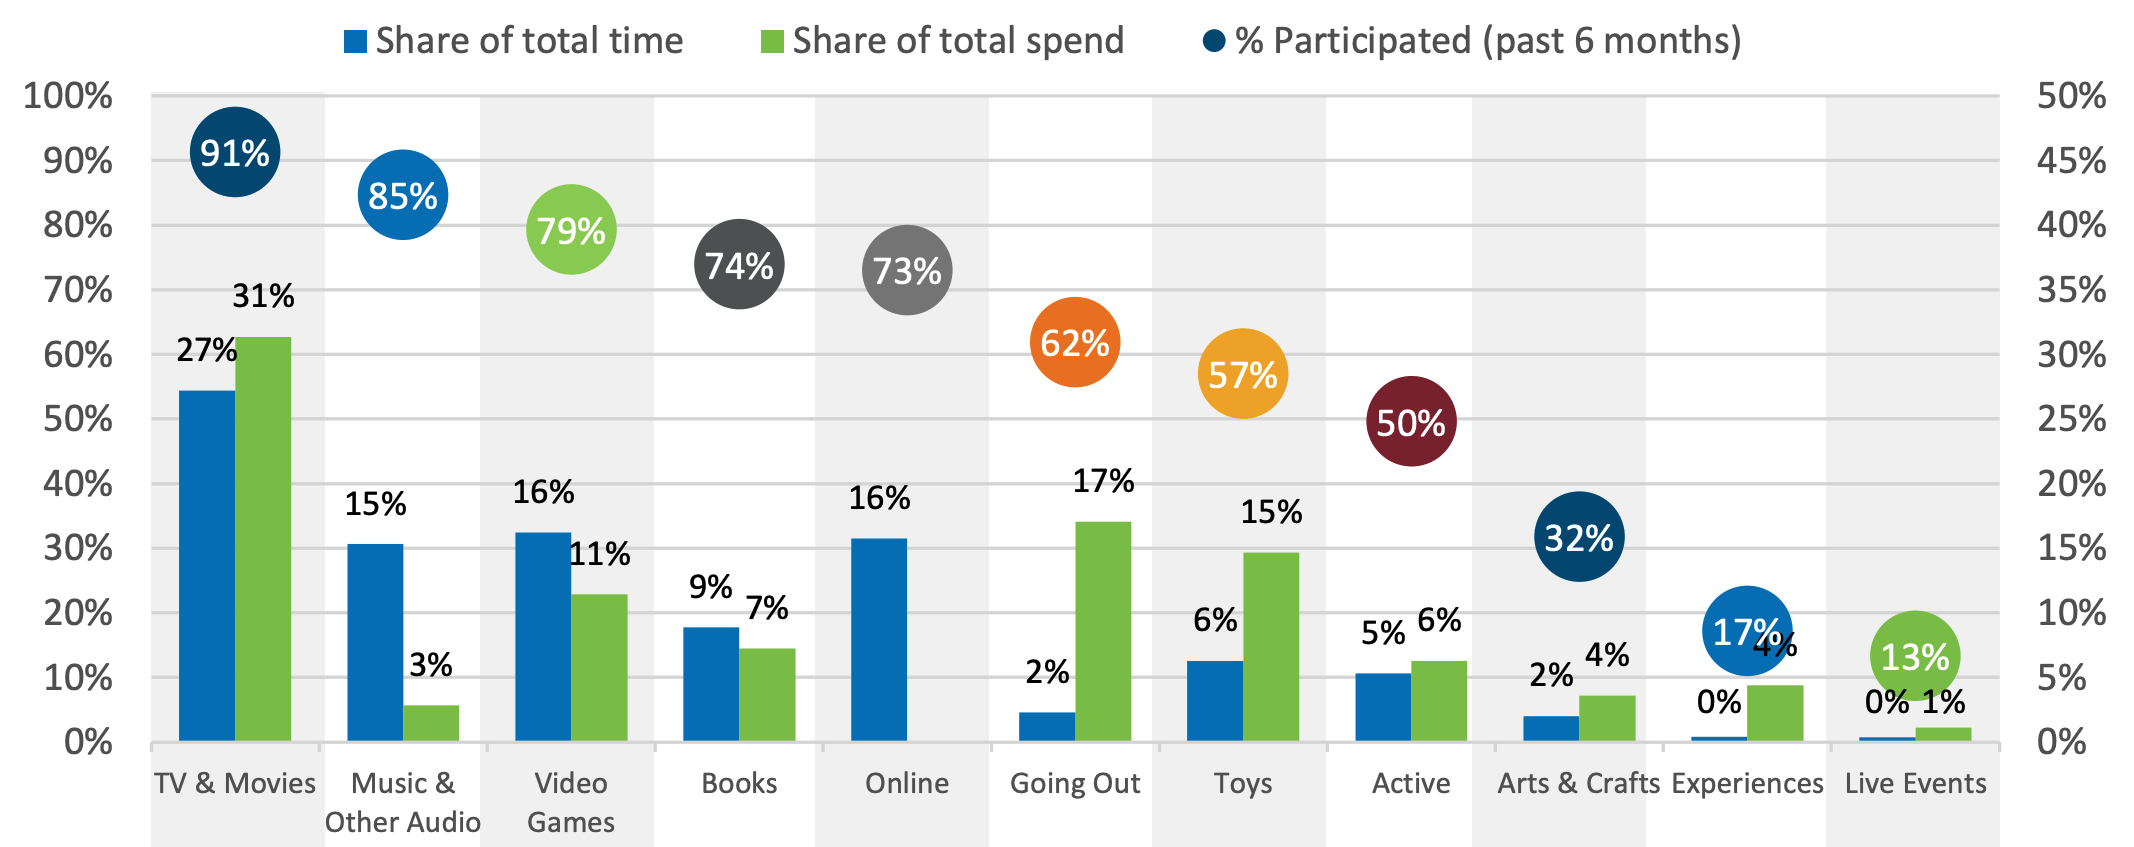
\includegraphics[width=\linewidth]{images/game.png}
    \caption{2020 Report on Entertainment Category Engagement; 79\% of the population is taken by gamers.\\ Source: 2020 Evolution of Entertainment / NPD Group}
    \label{fig:entertainment-report}
\end{figure}

Foldit, designed by researchers at the University of Washington, is a game in which gamers solve protein folding patterns, a central challenge in biochemistry, by virtually wiggling, shaking and pulling shapes to create small stable structures, as well as developing their own algorithms for solving protein folding \cite{bourzac2008enlisting}. This citizen science online game have had more than 800,000 registered players \footnote{As of 13/01/2021, \url{https://fold.it/portal/players}}, identified a potential target for HIV development, and redesigned a catalyst for the Diels-Alder reactions \cite{kreitmair2019citizen}. EyeWire is another example of the success of citizen science gamified environments. With more than 200,00 gamers from 145 countries, EyeWire allows users to map neurons in the retina, filling and extending areas missed by artificial intelligence \cite{kreitmair2019citizen}.

Once focused on ecological and environmental sciences, the citizen science practice has a much larger range now, covering topics such as linguistics \cite{svendsen2018dynamics}, astronomy \cite{marshall2015ideas}, hydrology \cite{buytaert2014citizen} etc. Out of these interest areas, one that could see further development with initiatives using citizen science is Natural Language Processing.

Natural language processing is a vast field that explores how computers can understand and manipulate human language in text or speech format. Researches in this area include (but are not limited to) sentiment analysis, sentence prediction, text translation, text-to-speech conversion, and speech recognition.

Also known as automatic speech recognition (ASR), computer speech recognition, or speech-to-text (STT), speech recognition is a field that studies the recognition and translation of spoken language into text by computers. It has been an intensive research area for decades, but has seen growth led by increased demand on ASR systems in the mobile environment \cite{yu2016automatic}, with virtual assistants, such as Alexa, Siri, Google Now.

Speech recognition is a class of machine learning that has seen many different approaches over time: stochastically modelling with Hidden Markov Models  \cite{gales2008application}, artificial intelligence learning with Neural Networks \cite{graves2013speech}, non-stochastical modelling \cite{burget2003nonrandomattr} and even hybrid approaches \cite{wang2020transformer} have been made to solve this complex interdisciplinary field.

However, these voice modeling strategies are highly dependant on the quality and quantity of data provided. Factors such as noisy speech data, nonhomogeneous recordings, different microphones within the same dataset, and even speech disorders could limit proper analysis, affect accuracy, and even change speech predictions \cite{wrong}. 

These voice datasets, also known as Speech Corpus (or Speech Corpora in plural), curate a collection of audio recordings of a spoken language. Some of them also have additional text files with transcriptions of the words spoken. Although they are widely found in the literature with robust recording procedures and analysis - such as TIMIT \cite{Lamel1992timmit}, DIRHA \cite{Ravanelli2016dirha} and the more recent \cite{chanchaochai2018globaltimit}) -, these datasets are structured in such a way that the speakers are individually selected. This could lead to bias problems \cite{bender2018data}, but also limits the number of voices recorded. Unfortunately, most speech corpora are recorded for the English language \cite{LeRouxVincent2014TRdatasets} and research is limited on the data quantity necessary to enable speech recognition systems and other voice applications.

To circumvent the quantity issue, some corpora are able to be constantly updated with user input. These online datasets can be accessed via web browser. Some examples are Vox Forge and Common Voice \cite{ardila2019common}. However, the former has poor user interface and little usage over time, and the latter has no structured analysis on bias mitigation, relying on crowdsourced information.

This work identifies the Citizen Science practice as a potential candidate to create a robust Speech Corpus for the low-resource Brazilian Portuguese language. A gamifyied application will be constructed to collect the data and engage users, applying data validation techniques to mitigate bias problems afterwards. The curated data will be published in a open-source platform to further research on speech recognition in this low-resource language.

\section*{Objective}

The main focus of this project lies in the construction and validation of a speech corpus for the brazilian portuguese language. The validated corpus and anonymized data will be available to the public.

\chapter{Method}

To achieve the aforementioned objective, this project will:

\begin{itemize}
    \item Research what characterizes a speech corpus in the literature;
    \item Create a list of phrases from which the public will read;
    \item Construct a application to record anonymized speech data;
    \item Add gamification elements to enhance public engagement;
    \item Validate recorded data and apply statistical methods to ensure data quality
    \item Publish dataset on open source platform
\end{itemize}

\section{Document structure}

This document is divided in 4 chapters:

\begin{itemize}
    \item Chapter 1 presents the context, motivation, and objective of the proposed research
    \item Chapter 2 details the background and foundation of all areas related to this research
    \item Chapter 3 presents related work on corpus creation
    \item Chapter 4 presents the systematic literature review to understand what characterizes a speech corpus
    \item Chapter 4 contains the proposed work to finish this research
\end{itemize}

	% ----------------------------------------------------------

% 	% ----------------------------------------------------------
% 	% Metodologia
% 	% ----------------------------------------------------------
	\chapter{Background}
\label{chap:background}

In this chapter, topics such as citizen science, gamification, and speech corpus will be further described. Additional terms relevant to the research will also be defined and clarified, to ensure all research topics are clear. 

\section{Citizen Science}

\subsection{Origins}

The citizen science practice, although not formally defined as so, date back at least a couple of millennia. In ancient China, migratory locusts frequently destroyed harvests, and residents have helped to track outbreaks for some 2,000 years \cite{irwin2018no}. More recently, in 1890, citizen contribution was adopted by the Cooperative Weather Service \cite{quayle1991effects}, where amateurs send collected weather data to the National Weather Service, and continues to provide such data. Later in 1900, the ornithologist Frank Chapman proposed a new holiday tradition - a "Christmas Bird Census" \cite{harden1985christmas}, in which the public would count sighted birds in a predefined area. The Christmas Bird Count contributed to more than 200 publications in the scientific field \cite{kosmala2016assessing}, and the data collected assists the assessment of the health of bird populations, as well as help guide conservation action. In 1966, a similar census started by the North American Breeding Bird Survey contributed to more than 670 publications. The UK Butterfly Monitoring Scheme \cite{pollard1994monitoring}, started in 1976, assess trends in the abundance of butterflies within the United Kingdom, and have supported more than 100 publications.

\subsection{Definition}

The term "Citizen Science" was formally used by Alan Irwin, a sociologist now based at the Copenhagen Business School, with his book "Citizen science: A study of people, expertise and sustainable development" \cite{irwin1995citizen}. Irwin defined citizen science both as “science which assists the needs and concerns of citizens” and as “a form of science developed and enacted by the citizens themselves”. This term was soon modified to describe "a research technique using members of the public to gather or analyze data" \cite{bonney2009citizen}. However, with so many forms of contribution, citizen science now takes a more flexible concept, which can be adapted and applied within diverse situations and disciplines. To encompass this flexibility, the European Citizen Science Association \cite{robinson2018ten} set out some key principles which as a community they believe underlie good practice in citizen science. Appendix \ref{app:ten-principles} lists all ten principles.

\subsection{Classifications}

Below are some classifications in which citizen science projects can be divided:

\subsubsection{Volunteer Involvement}

An initial classification based on volunteer involvement \cite{follett2015analysis}: 
\begin{itemize}
    \item Contributory, where participants contribute to data collection and sometimes help analyze and disseminate results
    \item Collaborative, where citizens also analyze samples, design the study, interpret the data, draw conclusions and disseminate results
    \item Co-created, where they participate in all stages of the project, including defining questions, developing hypotheses, drawing conclusions, discussing results and answering new questions
\end{itemize}

\subsubsection{Goals of the study}

An alternative classification for these initiatives has been suggested by \cite{wiggins2011conservation}, and is based on the goals of the study:

\begin{itemize}
    \item Action projects, initiated by volunteers designed to encourage intervention in local concerns;
    \item Conservation projects, addressing natural resource management goals;
    \item Investigation projects, focusing on scientific research goals in a physical setting;
    \item Virtual projects, also focusing on scientific goals, but entirely based on information technology with all volunteer interaction occurring online;
    \item Education projects; often performed in the classroom or school grounds as part of the science curriculum.
\end{itemize}

\subsubsection{Topic of study}

An additional way of classifying citizen science projects is based on the topic of study, for example, astronomy, archaeology, and biology \cite{wiggins2011conservation}. 

\subsubsection{This work}

If these classifications are to be applied in this work, it should be categorized as a \textbf{contributory virtual speech corpus} citizen science project.

\section{Gamification}

Gamification has been a trending topic as a means of supporting user engagement, being commonly employed in the private sector but also in education, health, government, and science, taking advantage of the widespread activity of game playing \cite{kreitmair2019citizen}. The desire of gamifying services and businesses lies in bringing positive, intrinsically motivating \cite{ryan2000self}, "gamefull" experiences \cite{huotari2012defining} into a service. In the following sections, gamification is (1) defined accordingly to the literature, (2) established through motivational affordances - or game elements, (3) and characterized by some psychological and behavioral outcomes.

\subsection{Definition}

Gamification is commonly defined as "the use of elements of game design in non-game contexts" \cite{deterding2011game}. Although simple, this definition incorporates the succinct method used by gamification. An alternative interpretation by \cite{huotari2012defining} states that gamification is "a process of enhancing a service with affordances for gameful experiences in order to support user's overall value creation". The latter conceptualization suggests the interaction of two actors: (1) the user (using the service) is the creator of value while (2) the service provider can merely provide affordances for the user to experience gamefulness.

\subsection{Motivational affordances (game elements)}

A literature review of empirical studies on gamification by \cite{hamari2014does} defines a list of 10 commonly motivational affordances implemented in table \ref{tab:motivational-affordances}. These 24 peer-reviewed studies were examined, indicating a large variety of different game elements added. The most commonly found were points, leaderboards and badges.

\begin{table}[h]
    \centering
    \caption{Quantity of tested motivational affordances in 24 gamification publications}
    \begin{tabular}{|c|c|}
        \hline Affordance & Publications (out of 24) \\
        \hline Points & 9 \\
        \hline Leaderboard & 10\\ 
        \hline Achievements/Badges & 9 \\
        \hline Levels & 6 \\
        \hline Story/Theme & 6 \\
        \hline Clear goals & 4 \\
        \hline Feedback & 6 \\
        \hline Rewards & 4 \\
        \hline Progress & 4 \\
        \hline Challenge & 7 \\
        \hline
    \end{tabular}
    \caption*{Source: \cite{hamari2014does}}
    \label{tab:motivational-affordances}
\end{table}

\subsection{Psychological and behavioral outcomes}

\subsection{Crowdfunding}

\section{Citizen Science Projects}

With the recent growth of citizen science, various breakthroughs were made possible. Below are some of the most relevant projects in the virtual space, some of which apply gamification to engage contributors.

\subsection{Foldit}

\begin{figure}[ht]
    \centering
    \caption{Foldit - Unfolded (and unstable) Streptococcal Protein Puzzle}
    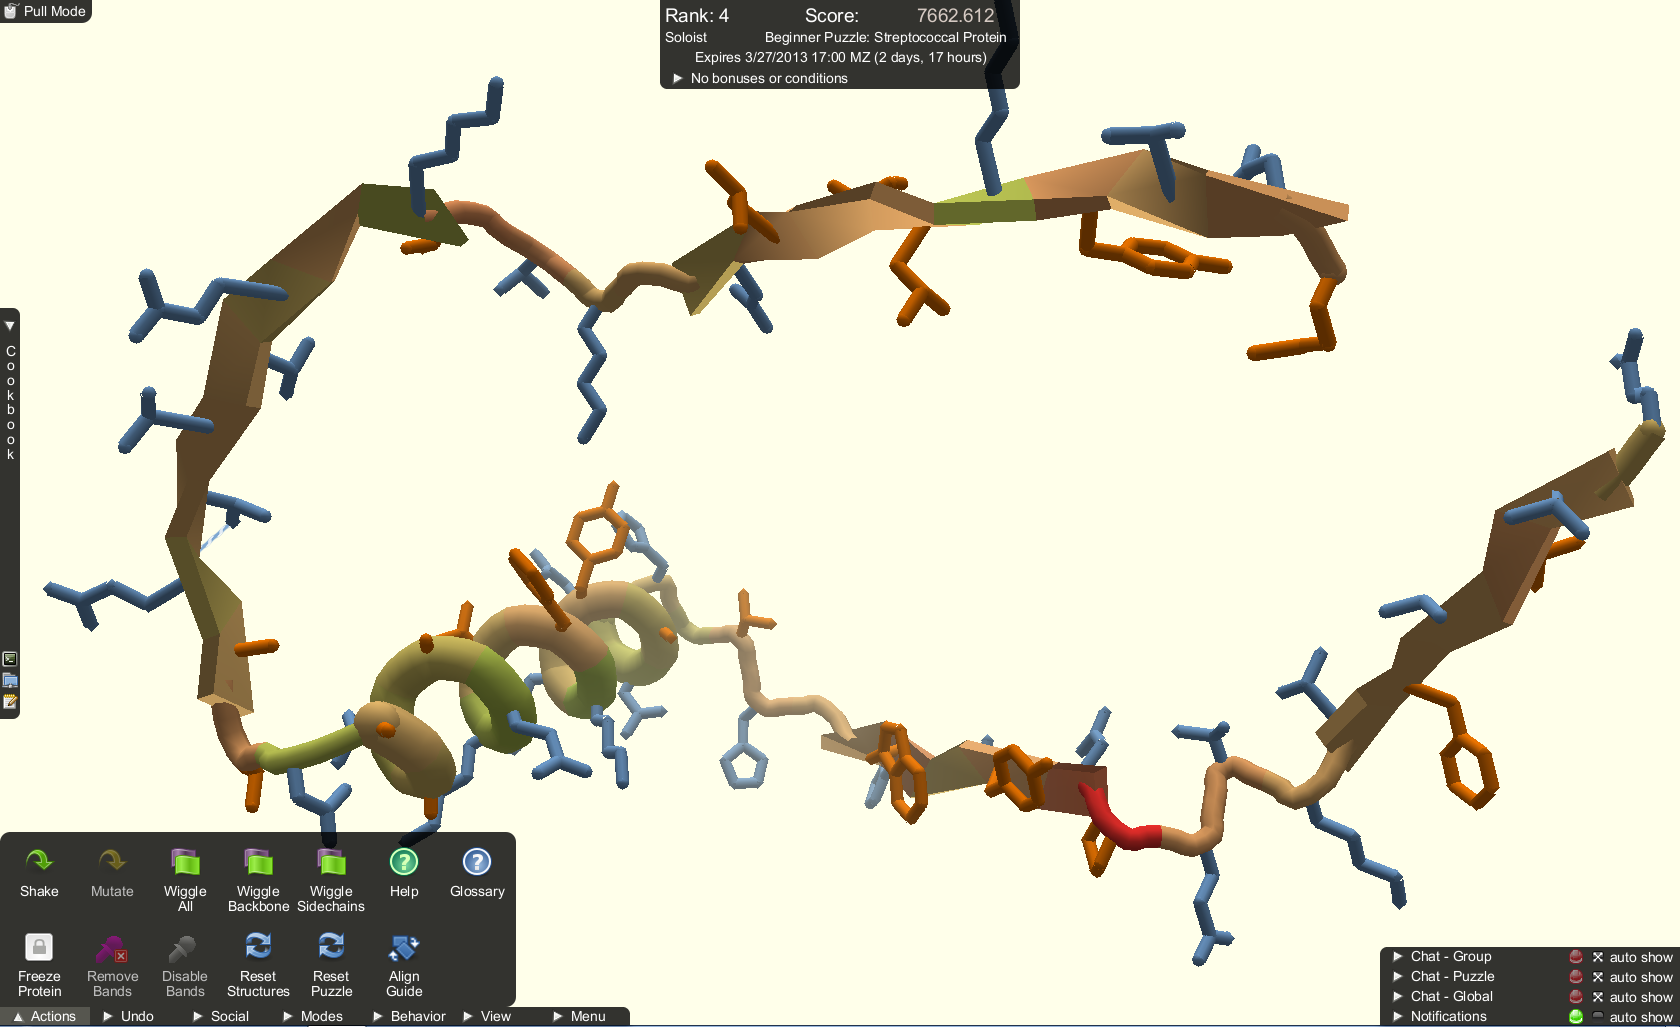
\includegraphics[width=0.8\linewidth]{images/background/foldit-problem.png}
    \caption*{Source: \cite{foldit-protein-problem}}
    \label{fig:foldit-problem}
\end{figure}

Foldit, designed by researchers at the University of Washington, is a game in which gamers solve protein folding patterns, a central challenge in biochemistry, by virtually wiggling, shaking and pulling shapes to create small stable structures, as well as developing their own algorithms for solving protein folding \cite{bourzac2008enlisting}. 

\begin{figure}[ht]
    \centering
    \caption{Foldit - Folded up Streptococcal Protein Puzzle}
    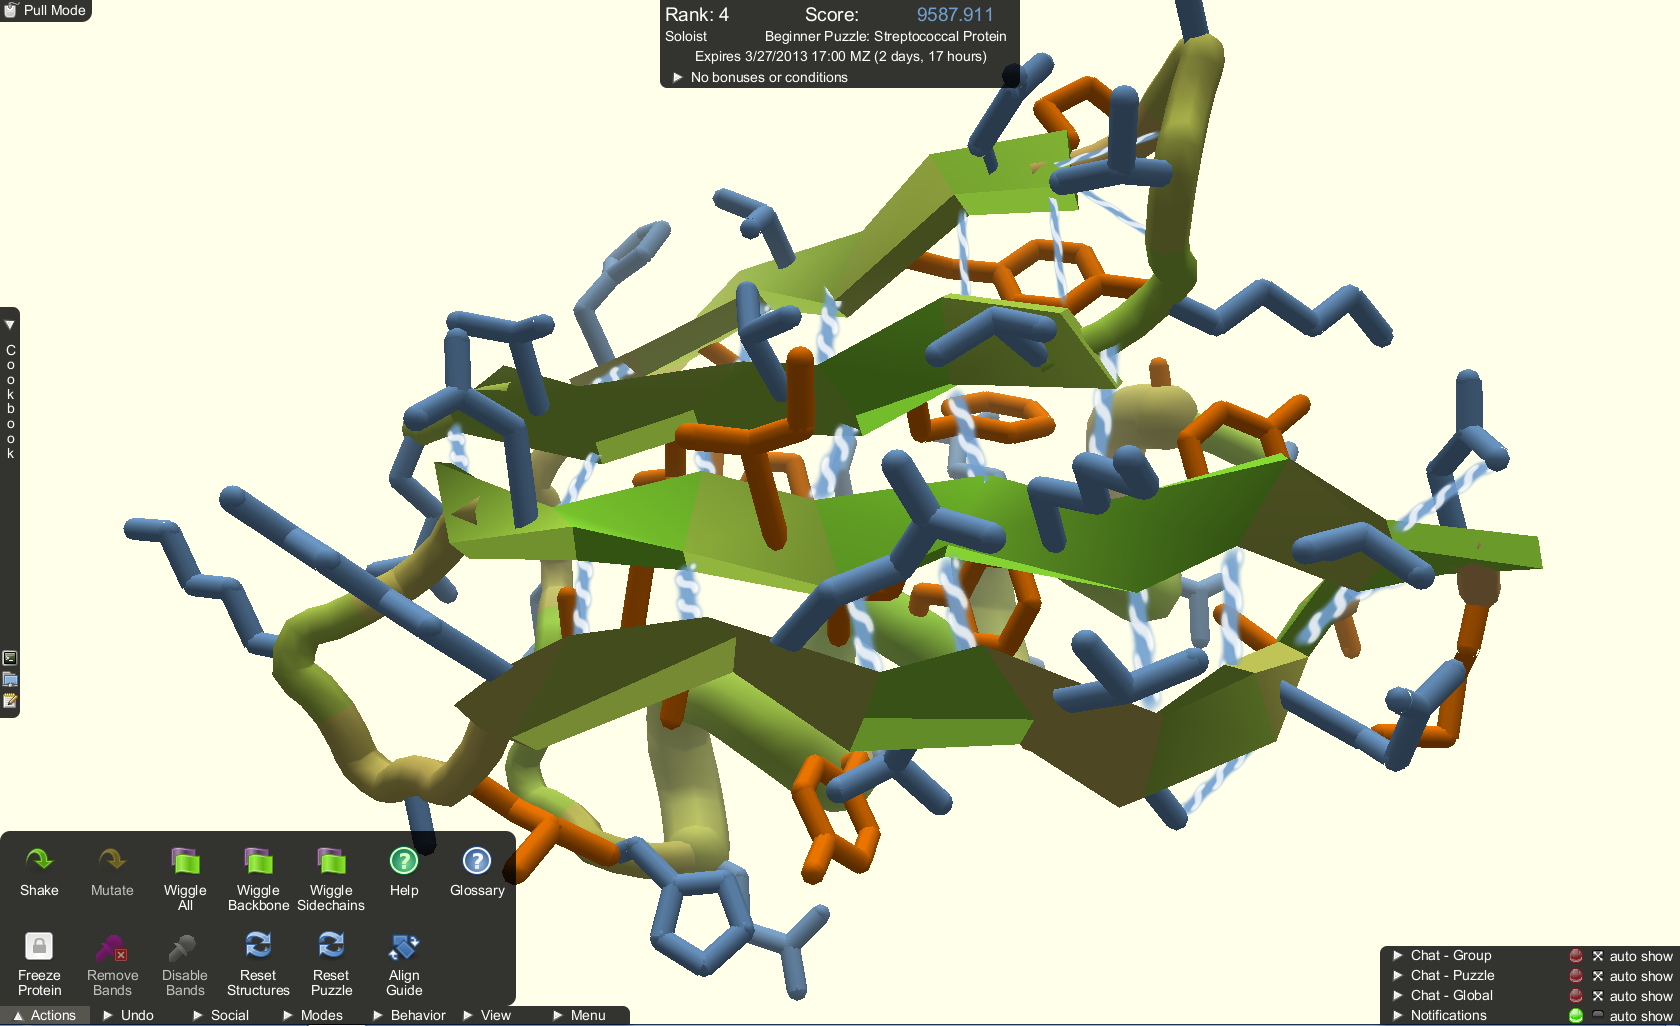
\includegraphics[width=0.8\linewidth]{images/background/foldit-solution.png}
    \caption*{Source: \cite{foldit-protein-solution}}
    \label{fig:foldit-solution}
\end{figure}

As the moment of this article, Foldit has had 20 peer-reviewed articles in a number of journals and conferences \cite{foldit2021publications}. Some relevant breakthroughs are a potential target for HIV drug development \cite{khatib2011crystal}, redesign of the catalyst for the Diels-Alder reaction \cite{eiben2012increased}, and improvement of cryo-electron microscopy atomic model building and refinement \cite{khatib2019building}.

\subsubsection{Gamification in Foldit}

To appeal to the general public, Foldit applies gamification in many different elements. The main objective of the game is to obtain the most stable and folded protein. To encourage this optimization, the user interface assigns a score to the protein, relative to how well it is folded. The best solutions to these puzzles are displayed in a ranking system, to promote competition between users. Another element to aid engagement is social. Users create and join groups, and members of groups can share puzzle solutions. These groups have been found to be useful in training new players.

\subsection{EyeWire}

\begin{figure}[ht]
    \centering
    \caption{EyeWire game interface}
    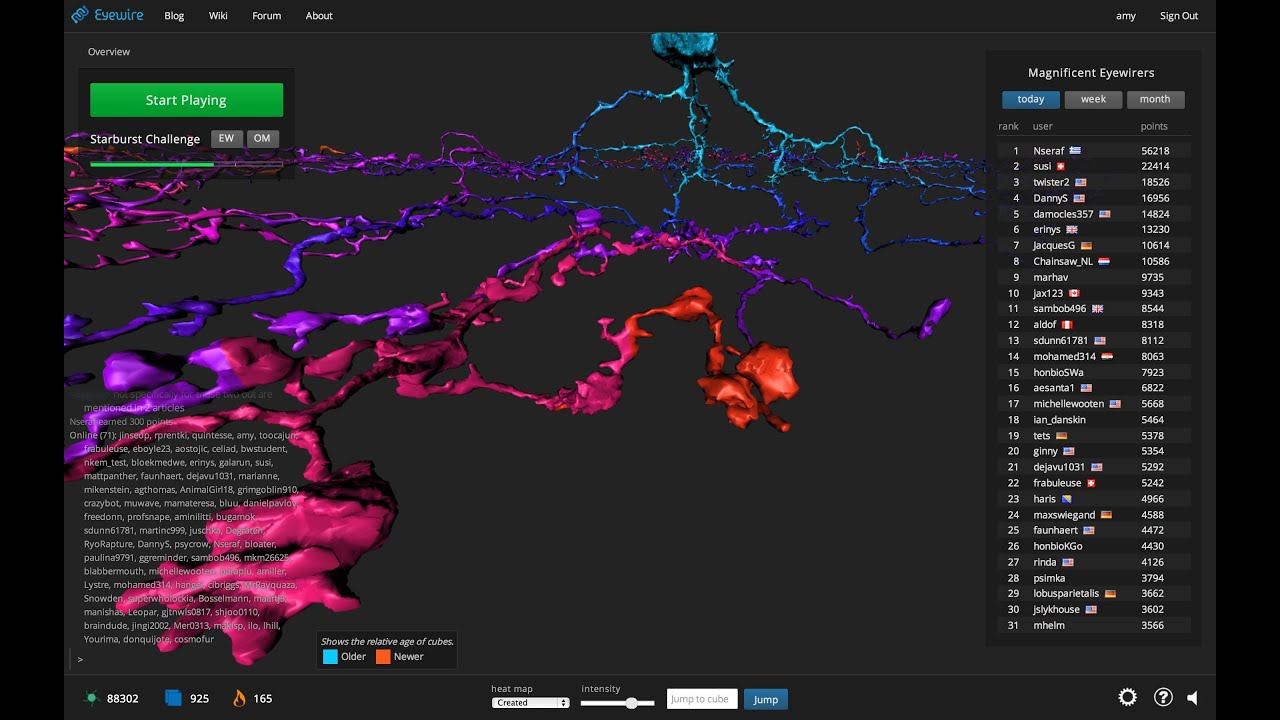
\includegraphics[width=0.8\linewidth]{images/background/eyewire.jpg}
    \caption*{Source: \cite{eyewire2014how}}
    \label{fig:eyewire-game-interface}
\end{figure}

EyeWire is a Web-based citizen science game that aims to create a detailed atlas of the human brain. Nonprofessionals are asked to map connections of neurons which reside in the back of the human eye. This mapping is done through 3D-transformed functional magnetic resonance images (fMRI), and combines crowd contributions with machine learning algorithms to help neuroscientists to achieve a better understanding of visual stimuli processing by humans.

\subsubsection{Gamification in EyeWire}

EyeWire transforms the complex task of brain mapping into smaller (micro) tasks via a gaming interface with several elements associated \cite{seaborn2015gamification}. This has been identified as a positive motivation for a player's participation \cite{tinati2016because}. Other elements such as music, sound effects, interactive tutorials, leaderboard, and a chat interface add to the overall experience, creating a fun experience. According to a survey on EyeWire motivation \cite{tinati2016because}, 57\% out of 349 respondents considered the the game entertaining.

\subsection{Galaxy Zoo}

\begin{figure}[ht]
    \centering
    \caption{Hubble's Galaxy Classification Schema to help new players classify galaxies}
    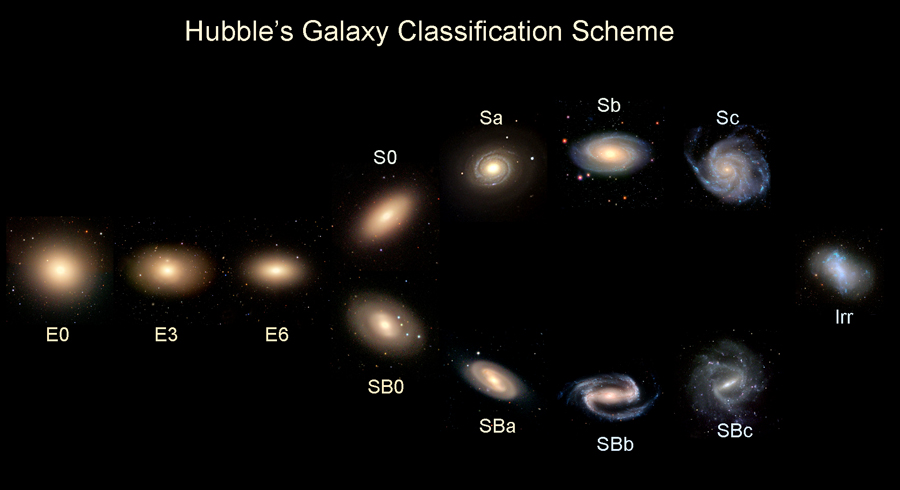
\includegraphics[width=0.8\linewidth]{images/background/galaxyzoo-training.jpg}
    \caption*{Source: \cite{galaxyzoo2010hubble}}
    \label{fig:galaxyzoo-hubble}
\end{figure}

In July 2007, Galaxy Zoo was a simple online citizen science initiative that asked volunteers to morphologically classify selected images of galaxies by the Sloan Digital Sky Survey (\cite{york2000sloan} executed at Apache Point Observatory by the SDSS 2.5m telescope). In this first iteration, Galaxy Zoo has had more than 100,000 volunteers classifying nearly 900,000 galaxies \cite{lintott2011galaxy}. The unexpected popularity has inspired the creation of Zooniverse, hosting project using the same technique across many research areas \cite{zooniverse2021galaxy}.

After its end in 2009, Galaxy Zoo was followed by Galaxy Zoo 2 (GZ2). The second incarnation extends the original Galaxy Zoo classifications for a subset of the brightest galaxies in the legacy release, measuring more detailed morphological features. This iteration contributed to 60 million classifications on more than 250,00 SDSS galaxies by more than 80,000 volunteers \cite{galaxyzoo22021volunteers}.

Including the latest issue of Galaxy Zoo (started in 2018), the initiative has supported the publication of 82 articles \cite{galaxyzoo2021publications}, helping analyze elements such as: galaxy rotation, color of elliptical galaxies, galaxy dust, galaxy bulges, etc.

\subsubsection{Gamification in Galaxy Zoo}

Galaxy Zoo utilizes the Zooniverse platform for data classification. This platform is not a gamified environment, thus relying on other forms of engagement to retain users, such as interest in astronomy, enjoyment of looking at galaxy pictures, desire and excitement to contribute to scientific research, etc \cite{raddick2009galaxy}.

\subsection{Zooniverse}

\begin{figure}[ht]
    \centering
    \caption{Zooniverse Platform, connecting volunteers with scientists}
    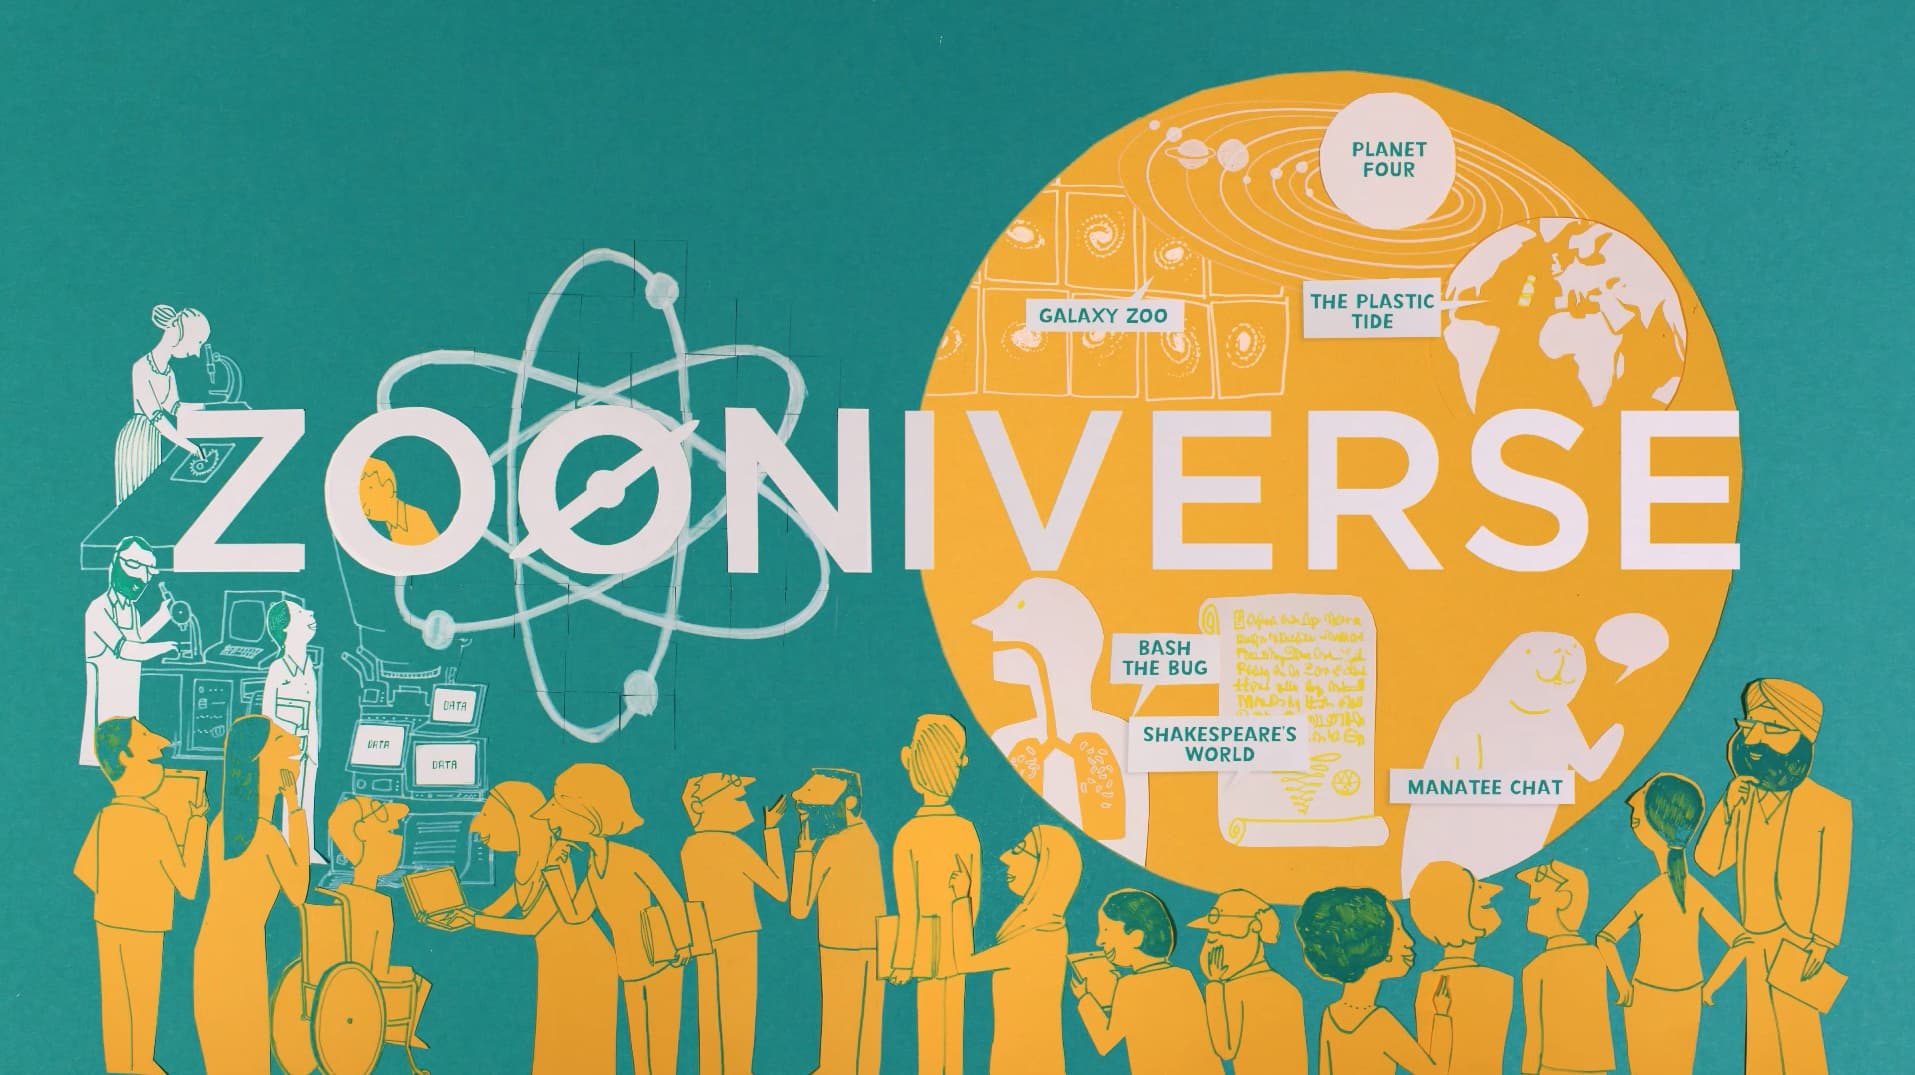
\includegraphics[width=0.7\linewidth]{images/background/zooniverse.jpg}
    \caption*{Source: \cite{zooniverse-logo}}
    \label{fig:foldit-solution}
\end{figure}

Zooniverse is a platform for citizen science projects. It connects more than a million volunteers around the world to assist professional researchers. The platform has a simple interface for input and classification of data, as well as the creation and management of projects.

This collaborative platform has enabled over 300 of scientific publications, with publications on the discovery and classification of stars, planets, supernovas; humanities, animal identification, classification of whale calls, datasets, etc. The following projects started in Zooniverse and each have their own characteristics:

\subsection{Penguin Watch}

\begin{figure}[ht]
    \centering
    \caption{Penguin Watch interface - Penguins are marked as adults and chicks}
    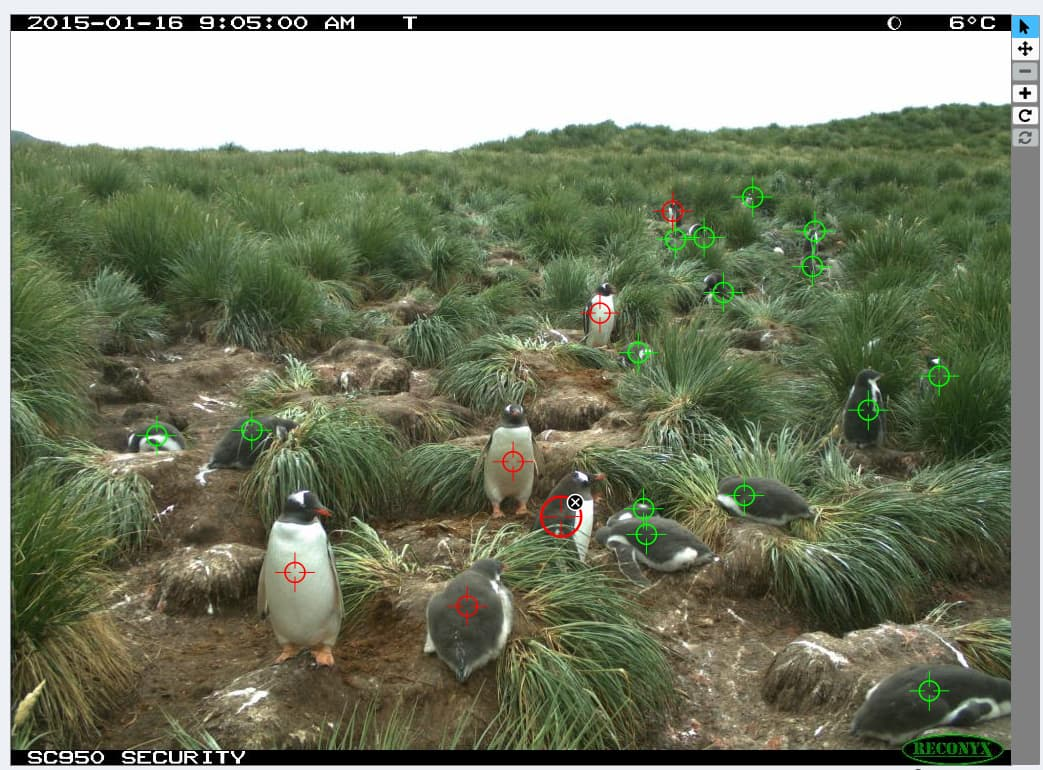
\includegraphics[width=0.8\linewidth]{images/background/penguinwatch.jpg}
    \caption*{Source: \cite{penguin2015watch}}
    \label{fig:oldweather-logbook}
\end{figure}

The Penguin Watch citizen science project states that by monitoring the population change in seabirds like penguins, it is possible to identify changes occurring in the wider ecosystem. These changes can help create health indicators of the marine environment, but the lack of the ability to collect and analyze such amounts of data made a team of researchers create the Penguin Watch initiative. Contributors help identify penguins in images of various sites over the world by using a web interface in Zooniverse.

\subsubsection{Gamification in Penguin Watch}

Like with GalaxyZoo, Penguin Watch runs their contribution platform over Zooniverse. While the platform does take responsibility in maintaining infrastructure and service management, it does not include gamification elements in the classification interface.

\subsection{Contributions}

The table \ref{tab:cs-contributions} contains an aggregated list of contributors and contributions from the projects described above.

\begin{table}[h]
\centering
\begin{threeparttable}
    \caption{Contribution for online citizen science projects}
    \small{
    \begin{tabular}{|c|c|c|}
        \hline 
        Project & Contributors & Publications \\ \hline
        Foldit & 855,350 \cite{foldit2021players} & 20 \cite{foldit2021publications} \\ \hline
        EyeWire & 300,000 \cite{eyewire2017players} & 3 \cite{eyewire2021publications} \\ \hline
        Penguin Watch & 28,500 \cite{penguin2021players} & 10 \cite{penguin2021publications} \\ \hline
        Galaxy Zoo (2007-2009) & 100,000+ \cite{lintott2011galaxy} & \multirow{3}{*}{82 \cite{galaxyzoo2021publications}\tnote{~a}} \\ \cline{1-2} 
        Galaxy Zoo 2 (2009-2013) & 80,000+ \cite{galaxyzoo22021volunteers} & \\ \cline{1-2} 
        Galaxy Zoo (2018-2021) & 61,149 \cite{galaxyzoo2021players} & \\ \hline 
    \end{tabular}}
    \begin{tablenotes}
        \item[a] Across all Galaxy Zoo Iterations, including Radio and Supernova Galaxy Zoo.
    \end{tablenotes}
\end{threeparttable}
\caption*{Source: Author}
\label{tab:cs-contributions}
\end{table}

\section{Natural Language Processing}

\subsection{Speech Recognition}

\section{Speech Corpus}

\section{Noisy data}

A common issue with these croudsourced online datasets lies in data quality. Disparities in recorded noise, environment change, recording length variation, and general quality of the recording are intrinsically associated with these contributions, since volunteers have each their own devices and recording conditions. To mitigate these issues, work has been made in the post-processing of these recordings \cite{krishna2019speech}.

\section{Licencing}
\subsection{GPL}
\subsection{CC0}

\section{Systematic Literature Review}


	\chapter[Related Work]{Related Work}

In this section, we discuss how the literature has treated speech corpora creation, as well as the various conditions and variables considered in the process. Speech Corpus crafting itself is well established in the literature by TIMIT \cite{Lamel1992timmit} and SWITCHBOARD \cite{godfrey1992switchboard}. TIMIT creates a dataset of 6300 utterances by 630 speakers from different regions of the United States. The sentences were crafted to fit in one of the three categories: 1) dialect "shibboleth", 2) phonemically compact and 3) phonetically diverse, but the selection itself was not well defined. Nevertheless, it is a very robust dataset with a time-aligned transcription and a usage guide to automatic speech recognition applications.

The CHiME articles \cite{christensen2010chime} \cite{barker2013pascal}, \cite{barker2018fifth} (and more), are also source of structured speech corpora creation, challenging researchers to better recognize speech within a everyday listening environment using multiple distant microphones. Since the focus of these works lies on nonoptimal recording conditions, detailed information on the noise background, noise level, recording style and speech material has been provided, as well as comprehensive postprocessing work.

A more recent work by \cite{chanchaochai2018globaltimit} attempts to extend the TIMIT functionality to other languages, by providing a method to create "TIMIT-like" datasets. These datasets are caracterized by having 1) Multiple (anonymously) identified speakers, 2) Wide range of phonetically representative inputs, 3) Wideband recordings with good acoustic quality, 4) Time-aligned lexical and phonemic transcripts and 5) Easily availability to anyone. The authors detail the speakers and sessions, the text corpus selection process, the recording procedures, as well as the transcription and alignment methods. At the moment, there have been five datasets created, with more planned or in progress.

	\chapter[Proposal]{Proposal}

This proposal focuses on detailing the necessary steps to the creation and publication of a crowdfunding speech corpus in Brazilian Portuguese. To this end, a virtual voice recording application will be developed (section \ref{sec:proposal-app}), focusing on adding gamification elements to enhance user engagement. Additionally, this application will also extract some relevant characteristics found in the systematic literature review in chapter \ref{chap:slr}. Once the construction is finished, the application will be released, allowing general public submission (in section \ref{sec:proposal-public-submission}). After the submission period, the collected data will be analyzed and compiled to a speech corpus (\ref{sec:proposal-data-analysis}), which will be publicized to an open-source repository in section \ref{sec:proposal-data-publication}.

\section{Application}
\label{sec:proposal-app}

This section details the conception, documentation, and development process of the voice recording application, coined "Fale Alguma Coisa". Below, it will at times be referenced as "app", short for application.

\begin{figure}[ht]
    \centering
    \caption{Fale Alguma Coisa app Logo}
    
\includegraphics[width=\linewidth/2]{images/app/logo.jpg}
    \caption*{Source: Author}
    \label{fig:falealgumacoisa-logo}
\end{figure}

\subsection{Concept}

The Fale Alguma Coisa app should provide an easy gateway for you to contribute your voice while having fun and learning various science facts and curiosities.

\subsection{Target Audience}

Directed towards anyone interested in learning and contributing to science.

\subsection{User Stories}

The development of most software starts with its documentation. This work chose a user story approach to project documentation and lists them below, categorized by epic.

\subsubsection{Usability}

\begin{itemize}
    \item I, as a citizen, would like to contribute my voice using my mobile devices and desktop computer.
\end{itemize}

\subsubsection{Homepage}

The homepage epic represents the user stories affecting the homepage, such as the splash screen, call to action button, terms of service, etc.

\begin{itemize}
    \item I, as an unregistered citizen, would like to view an animated introductory screen in the application, so that I feel more inside a native app.
    \item I, as an unregistered citizen, would like to know more about Fale Alguma Coisa from a explanatory text in the homepage, so that I understand more about the project.
    \item I, as a registered citizen, would like to easily go from the homepage to the sign-in page, so that I can login to my account.
    \item I, as an unregistered citizen, would like to click a call to action button to go from the homepage to the recording page from the homepage, so that I can contribute my voice.
    \item I, as an unregistered citizen, would like to read the terms of service and privacy policy of Fale Alguma Coisa, so that I understand better what the service has to offer and what kind of data will be recorded.
\end{itemize}

\subsubsection{Recording}

The recording epic represents the most important feature in the application, as the citizen will use it to record his voice. It also provides supporting features, such as skipping phrases and resuming the recording session.

\begin{itemize}
    \item I, as an unregistered citizen, would like to view and accept the terms of service before recording, so that I understand how my data is being used.
    \item I, as an unregistered citizen, would like to properly configure my microphone before recording, so that I can record without interruption.
    \item I, as a citizen, would like to read science phrases with definitions and curiosities, so that I learn about subjects as I am contributing.
    \item I, as a citizen, would like to read phrases grouped by theme, so that I can learn more from each subject as I am contributing.
    \item I, as a citizen, would like to read a tutorial explaining how to record, so that I learn how to properly record phrases.
    \item I, as a citizen, would like to see animations on each step of the recording (enter the page, start the recording, stop the recording), so that I feel more engaged with the application.
    \item I, as a citizen, would like to skip a phrase when I (1) do not know how to pronounce, or (2) find a foreign word, or (3) another specified reason, so that I only speak the correct phrases.
    \item I, as a unregistered citizen, would like to stop this recording session by returning home when clicking the logo and confirming the exit, so that I can resume it afterwards.
    \item I, as a registered citizen, would like to return to the dashboard after clicking the logo and confirming the exit, so that I can resume it afterwards.
\end{itemize}

\subsubsection{Dashboard}

The dashboard epic lists all user stories related to the dashboard page, where the user will be able to choose themes to record, open the menu, check his level, etc.

\begin{itemize}
    \item I, as an unregistered citizen, would like to easily register my data through a button click, so that I can enjoy all features of the logged area.
    \item I, as a registered citizen, would like to see my actions in a dashboard after logging in, so that I can better contribute to the project.
    \item I, as a registered citizen, would like to see a list of recommended themes to speak, so that I can choose one from the list.
    \item I, as a registered citizen, would like to view my progress level, so that I know how far have I progressed in my contributions.
    \item I, as a registered citizen, would like to open the menu, so that I know which are my possible actions in the app.
    \item I, as a registered citizen, would like to check notifications, so that I understand what happened while I was gone.
\end{itemize}

\subsubsection{Gamification}

\begin{itemize}
    \item I, as a registered citizen, would like to get 100 points when I record my first phrase, so that I can engage better in the application.
    \item I, as a registered citizen, would like to get 400 points when I record my first theme, so that I can engage better in the application.
    \item I, as a registered citizen, would like to get 300 points when I record subsequent themes, so that I can engage better in the application.
    \item I, as a registered citizen, would like to get 500 points when I register my data, so that I can better engage with the application.
    \item I, as a registered citizen, would like to measure my points through a level, so that I can more easily compare myself with other users.
\end{itemize}

\subsubsection{Social}

\begin{itemize}
    \item I, as a registered citizen, would like to know who are the top contributors in the space and where am I in the list, so that I can compete against them.
    \item I, as a registered citizen, would like to know where my friends are in a more customized leaderboard, so that I can compete against them.
    \item I, as a registered citizen, would like to add a friend, so that I can check them in the friends leaderboard afterwards.
    \item I, as a registered citizen, would like to check notifications, so that I can know what happened when I was away.
    \item I, as a registered citizen, would like to know when someone added me through notifications, so that I can add them back later.
    \item I, as a registered citizen, would like to refer friends to the application, so that I can play with them.
\end{itemize}

\subsubsection{Login and Registration}

\begin{itemize}
    \item I, as an unregistered citizen, would like to login (using social login - Facebook / Google) on the app, so that I can login later and save my progress.
    \item I, as a unregistered citizen, would like to register my anonymous data on my first login, so that I can provide better metadata to my recordings afterwards.
    \item I, as a registered citizen, would like to update my account data, so that I can provide accurate metadata to the recordings.
    \item I, as a registered citizen, would like to remove my account data (and my recordings, if necessary), so that I can remove my metadata from this application.
\end{itemize}

\subsection{Design}

To ensure the development of the application is effective, an iterative design approach was taken. First, ideas for the app shaped a conceptual user journey. Second, this journey allowed the creation of layouts, which then passed through a validation process. Then, if aligned with the application concept, the layouts were developed. Otherwise, another design implementation occurred, undergoing further validation.

\subsubsection{Color Scheme}

In color theory, colors are used to communicate meaning, but also affect mood, and perception \cite{agoston2013color}. The design color scheme defines a color palette to choose from when designing new elements. Applying the concept, a more colorful color scheme was chosen to lighten the mood of the application, as shown in figure \ref{fig:falealgumacoisa-color-scheme}.

\begin{figure}[ht]
    \centering
    \caption{Fale Alguma Coisa color scheme}
    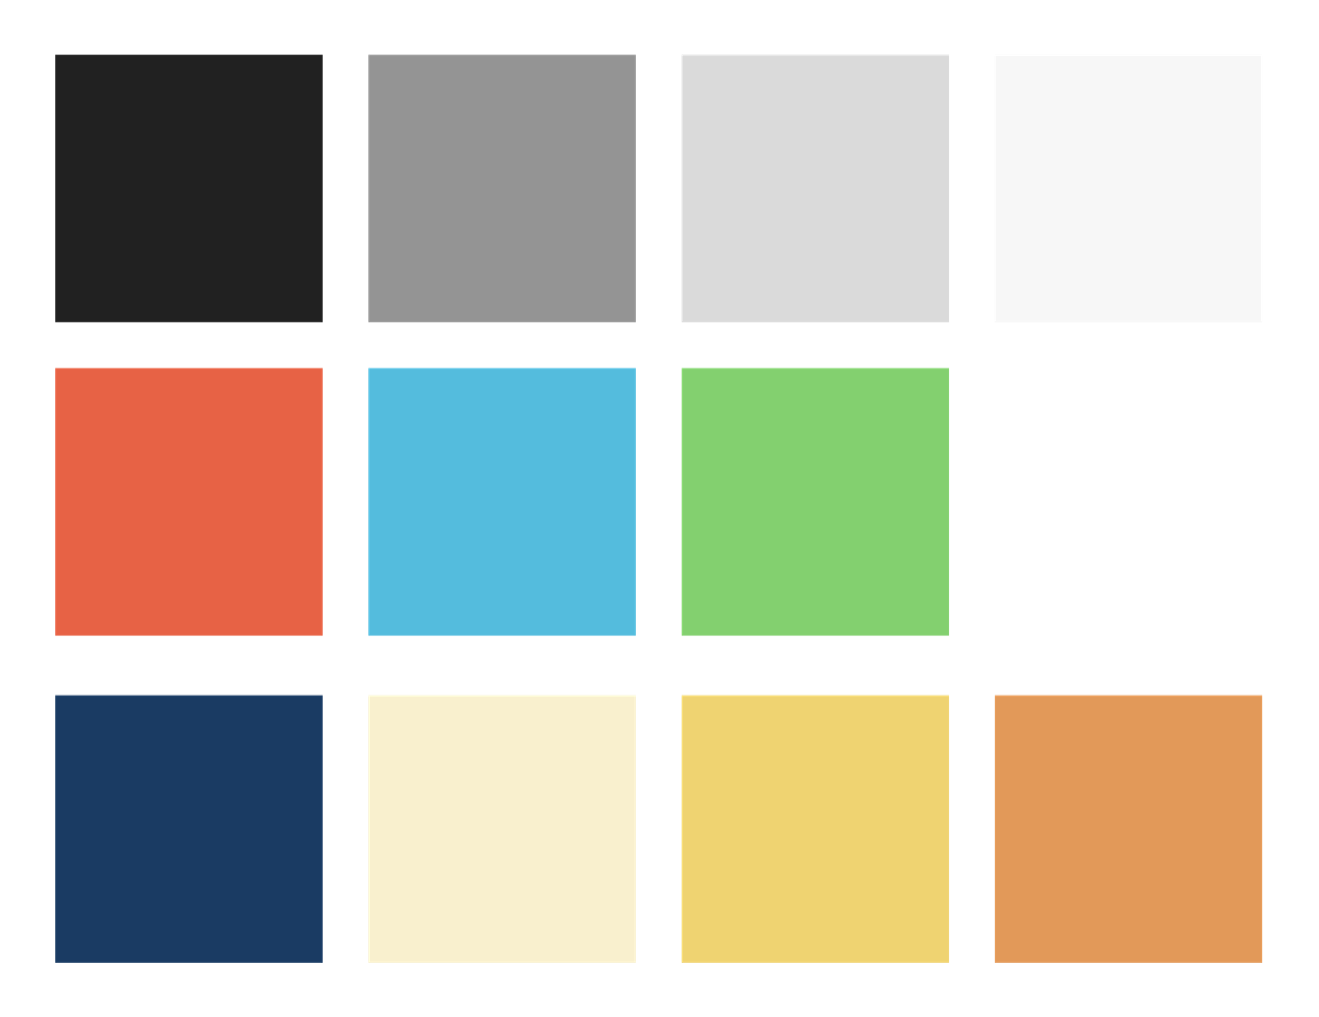
\includegraphics[width=\linewidth/2]{images/app/colors.png}
    \caption*{Source: Author}
    \label{fig:falealgumacoisa-color-scheme}
\end{figure}

\subsubsection{Web app}

To allow easier access to the voice recording app, a web-based application will be developed. This factor positively influences the capacity of the app to update over time, when compared to an application developed in a native environment. It also enables users over mobile and desktop to access the same application, and although the layout may have to be redesigned, most logic is reused.

\subsubsection{Mobile First}

The design will use a mobile first approach, to ensure the user flow will be optimized when he is using a mobile device. The desktop flow will be designed and developed afterwards.

\subsubsection{Splash Screen}

As the user first enter the application, a splash screen will be shown to welcome him (mobile version in figure \ref{fig:falealgumacoisa-splash-page-design}). It contains the logo and an animation to draw the user's attention. After the animation, the home will be shown.

\begin{figure}[ht]
    \centering
    \caption{Fale Alguma Coisa Splash Page design}
    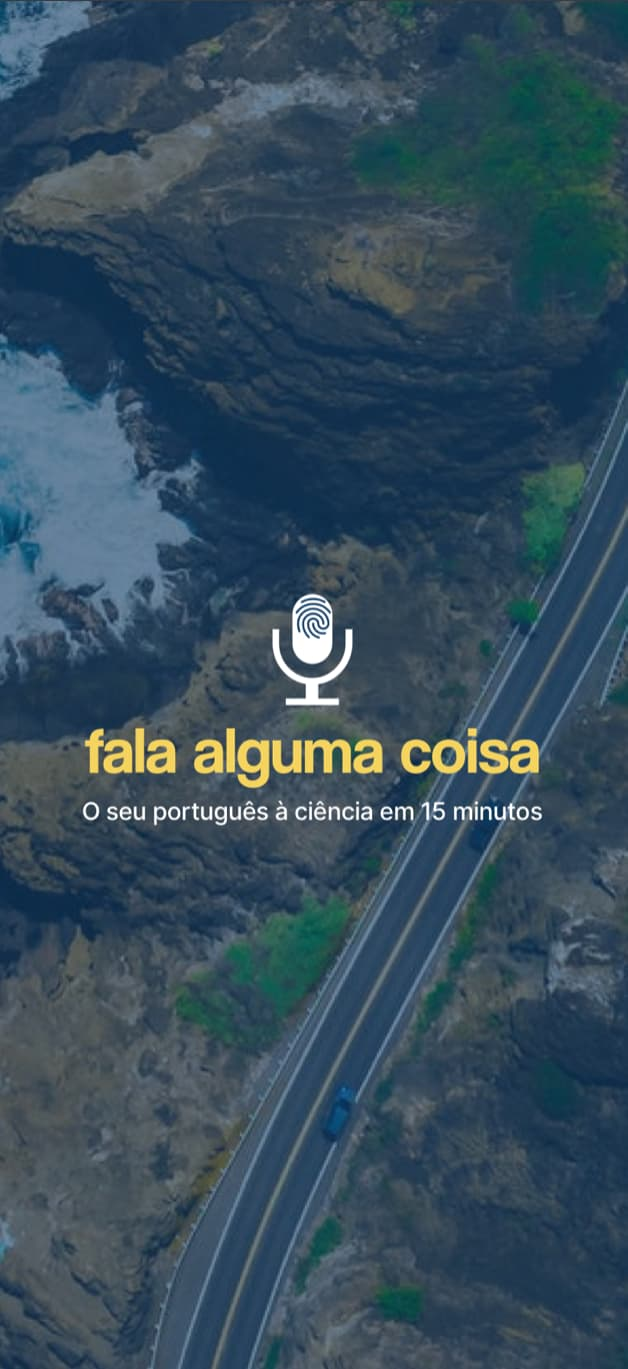
\includegraphics[width=\linewidth/2]{images/app/m-splash.jpg}
    \caption*{Source: Author}
    \label{fig:falealgumacoisa-splash-page-design}
\end{figure}

\subsubsection{Homepage}

After the splash animation, the homepage is shown. The mobile version can be seen below in figure \ref{fig:falealgumacoisa-home-page-design}. In this page, the call to action to start the recording is highlighted by the button at the center of the page, with text describing the project right below it. The login page is accessible through the link in the right upper corner. These few elements are placed to encourage the user to click on the recording, if he is a new user.

\begin{figure}[ht]
    \centering
    \caption{Fale Alguma Coisa Home Page design}
    \frame{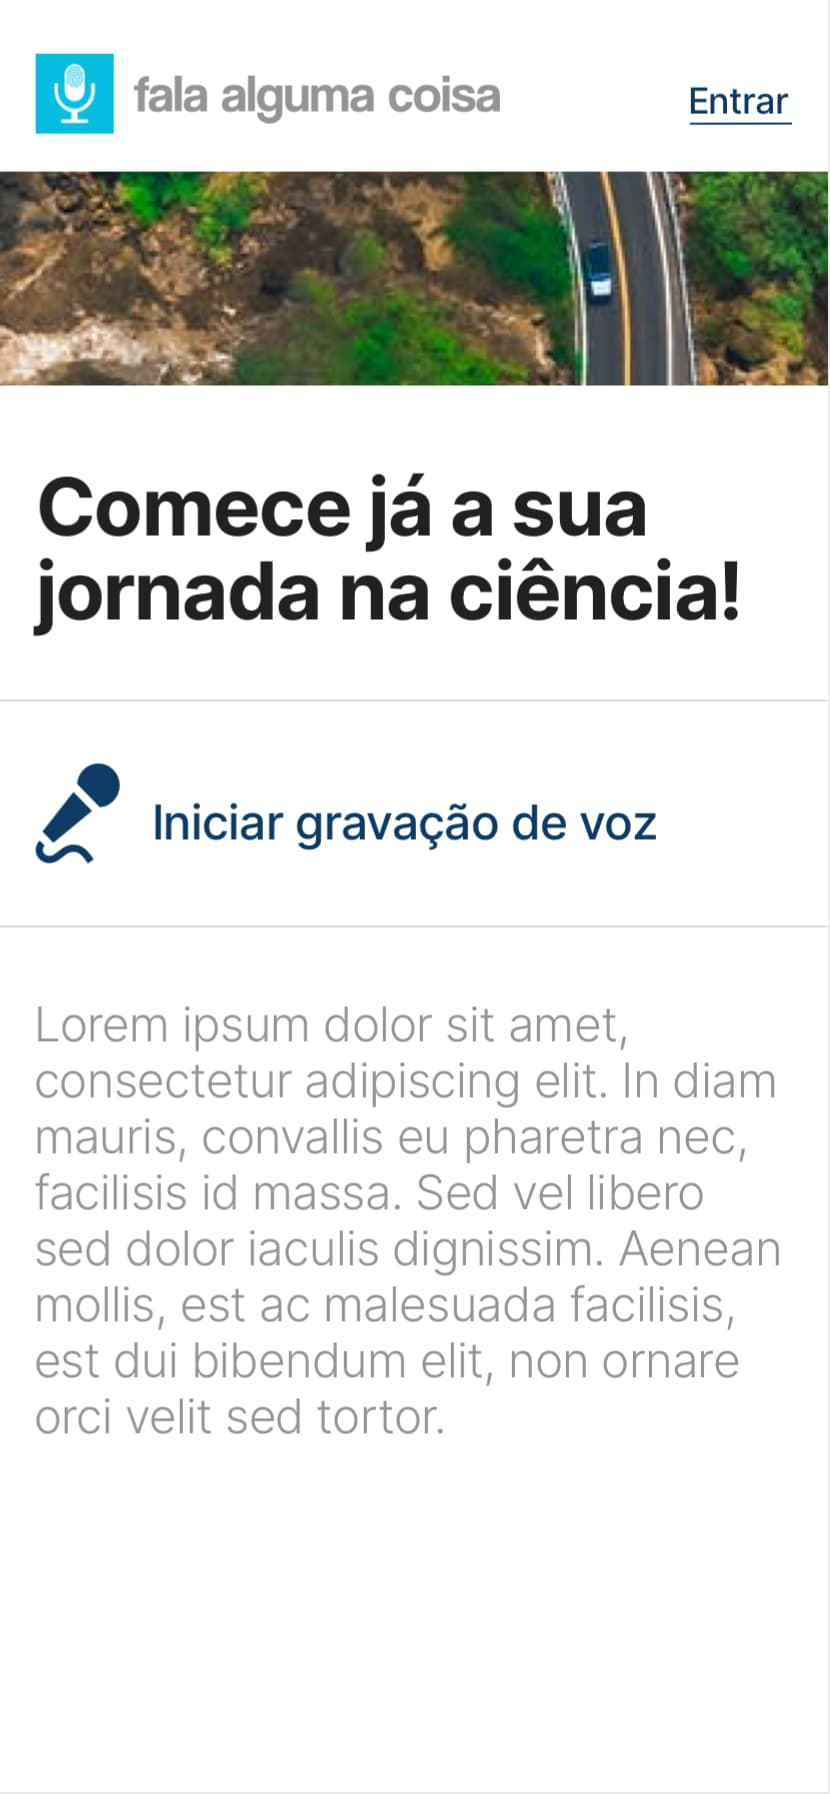
\includegraphics[width=\linewidth/2]{images/app/m-home.jpg}}
    \caption*{Source: Author}
    \label{fig:falealgumacoisa-home-page-design}
\end{figure}

\subsubsection{Recording}

This page represents the core functionality of the website, allowing the user to record phrases with his voice. The recording is done through groups of phrases, called a theme, and is illustrated by the image \ref{fig:falealgumacoisa-recording-page-design} at the bottom. The main elements of the page are (1) the phrase highlighted in a rectangular box at the center of the page, and (2) the red recording button at the bottom.

\begin{figure}[ht]
    \centering
    \caption{Fale Alguma Coisa Recording Page design}
    \frame{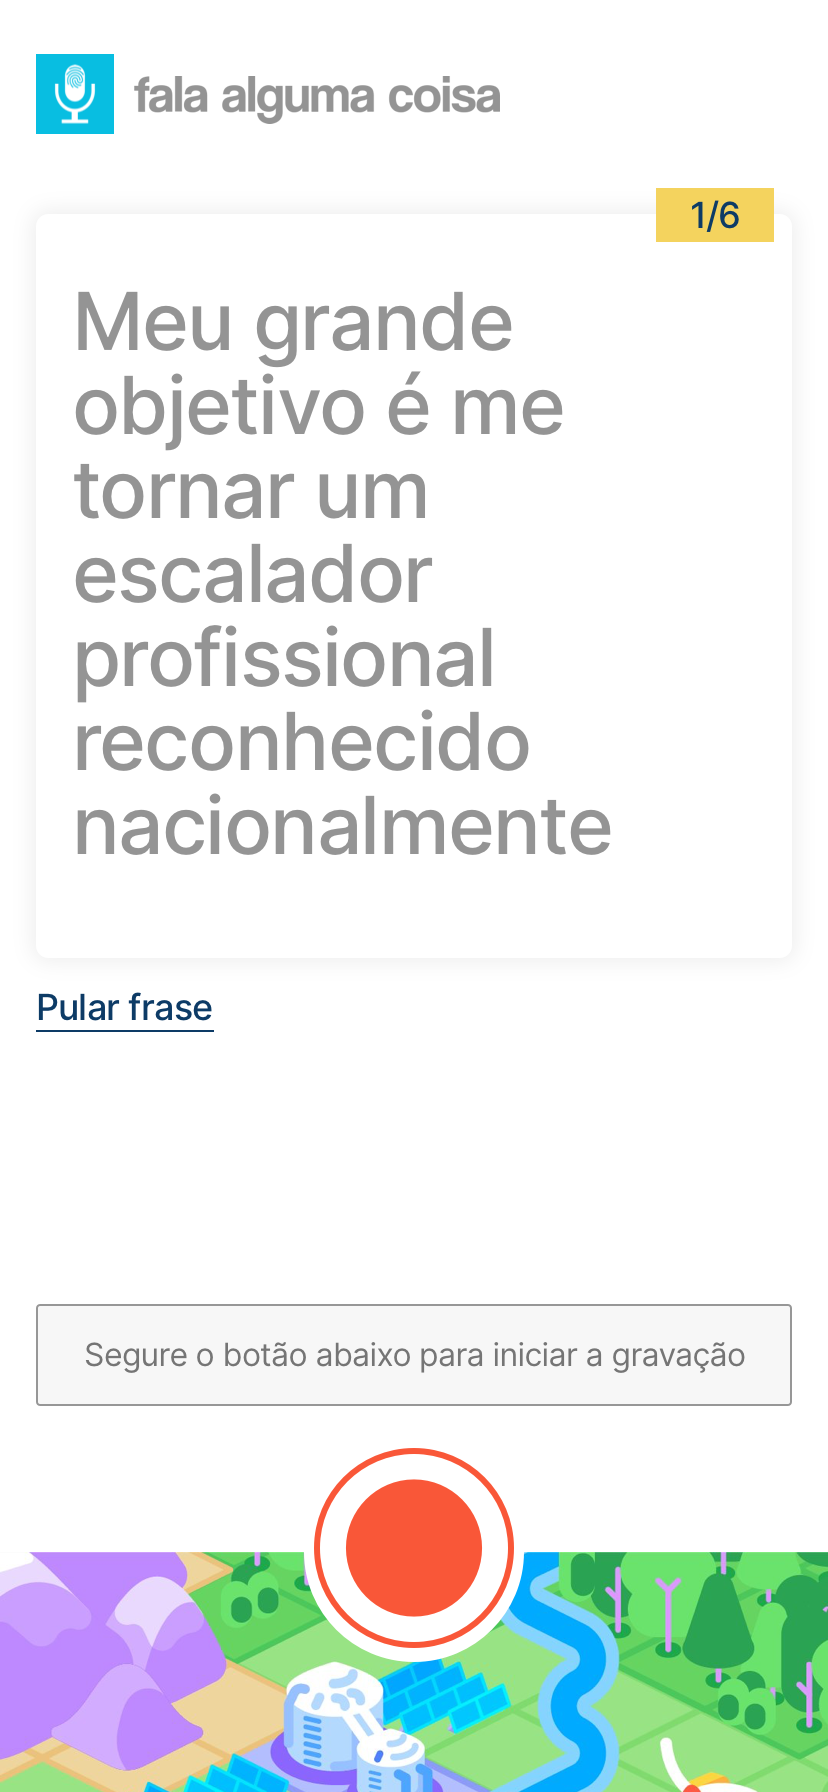
\includegraphics[width=\linewidth/2]{images/app/recording/Journey_1.0.png}}
    \caption*{Source: Author}
    \label{fig:falealgumacoisa-recording-page-design}
\end{figure}

\subsubsection{Dashboard}

When an unauthenticated user finishes recording its first theme, or when a user logs in, they are able to select from a list of themes to record. In this dashboard seen in figure \ref{fig:falealgumacoisa-dashboard-page-design}, they are also shown the number of points accumulated by the usage of the app, as well as able to open a menu and notification page.

\begin{figure}[ht]
    \centering
    \caption{Fale Alguma Coisa Dashboard Page design}
    \frame{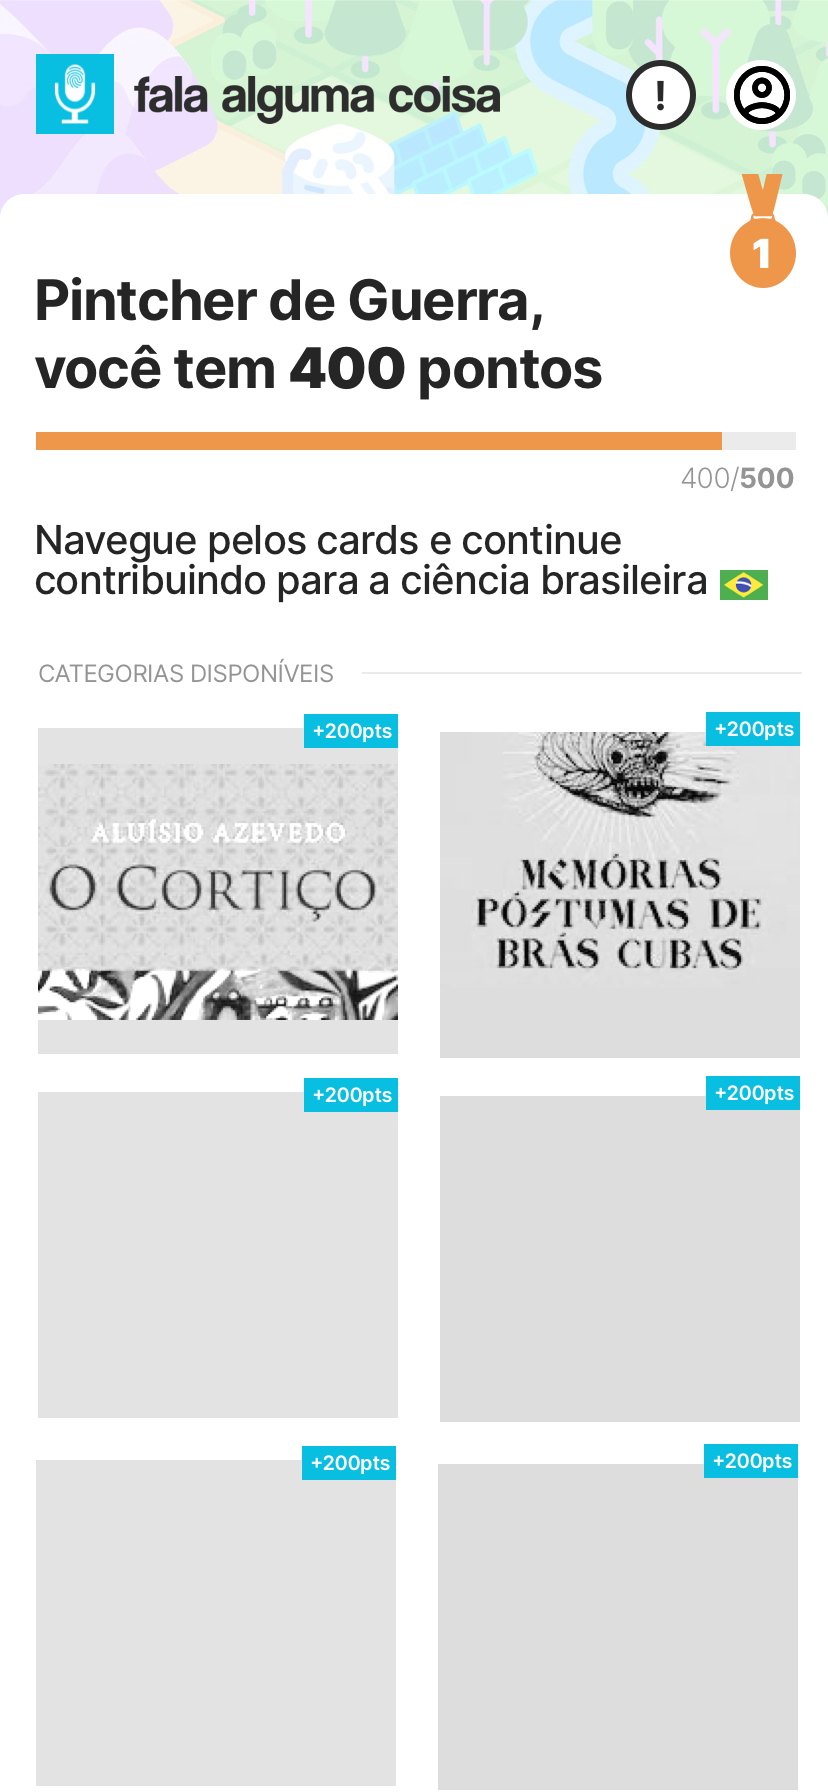
\includegraphics[width=\linewidth/2]{images/app/dashboard/Dashboard.png}}
    \caption*{Source: Author}
    \label{fig:falealgumacoisa-dashboard-page-design}
\end{figure}

\subsubsection{Leaderboard}

The leaderboard has two views: a list of the top ranking users (figure \ref{fig:falealgumacoisa-leaderboard-page-design-general}) and a list of friend rankings (figure \ref{fig:falealgumacoisa-leaderboard-page-design-friend}). They provide a way for users to compare their contributions, thus promoting competition. A social part is also included throughout the option to add friends.

\begin{figure}[ht]
    \centering
    \caption{Fale Alguma Coisa Leaderboard Page designs}
    \begin{subfigure}{.5\textwidth}
      \centering
      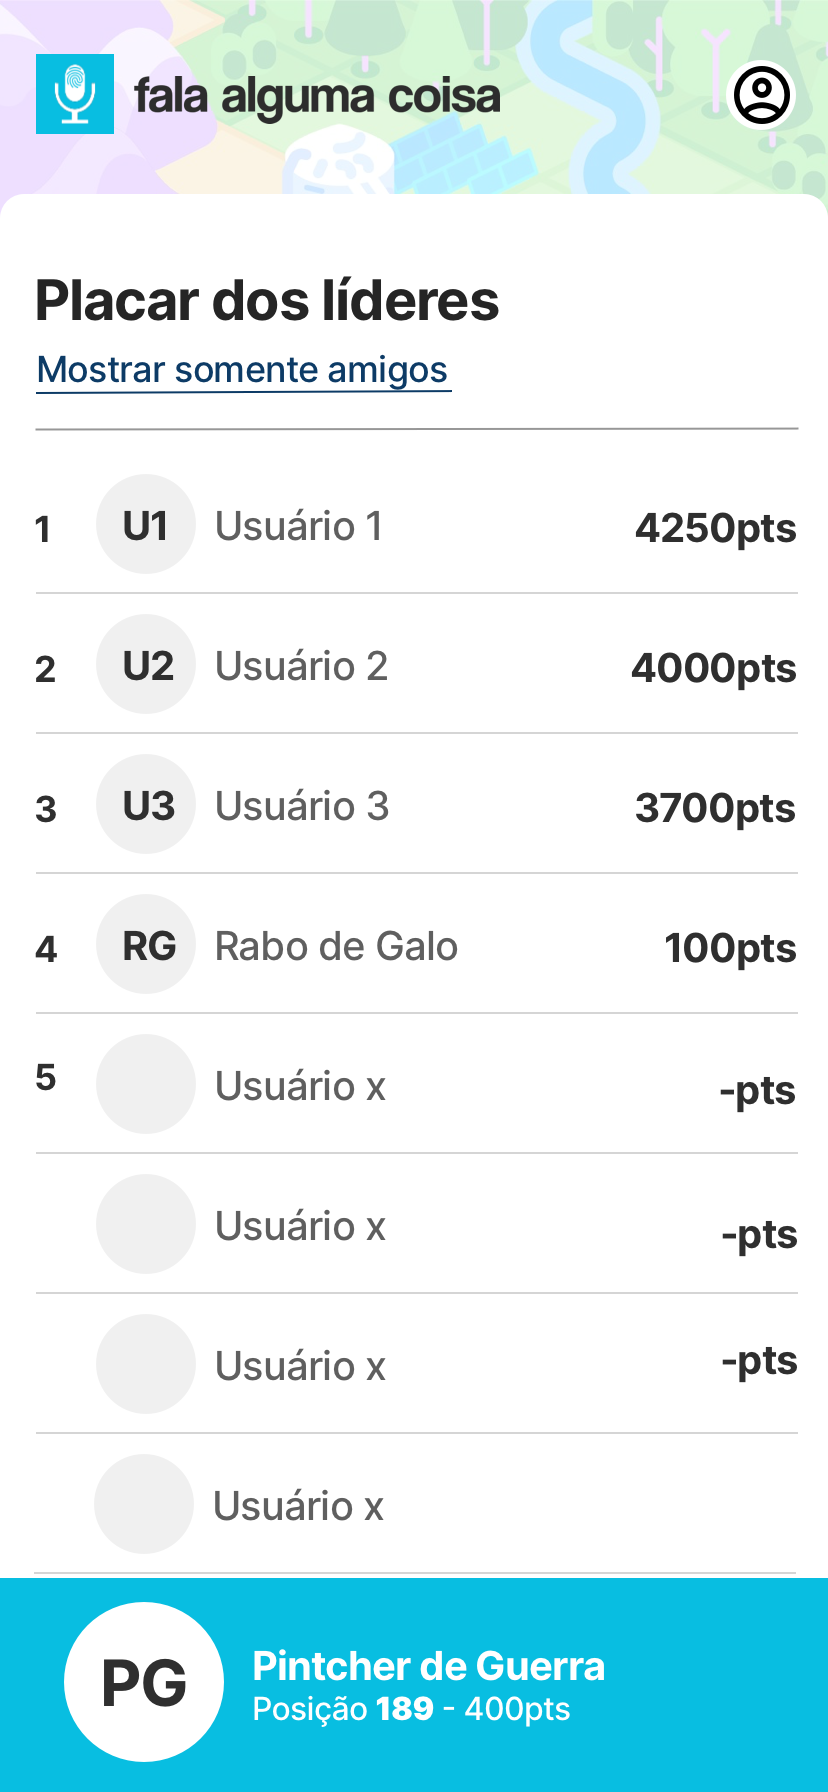
\includegraphics[width=.9\linewidth]{images/app/leaderboard/GeneralRanking.png}
      \caption{General Leaderboard}
      \label{fig:falealgumacoisa-leaderboard-page-design-general}
    \end{subfigure}%
    \begin{subfigure}{.5\textwidth}
      \centering
      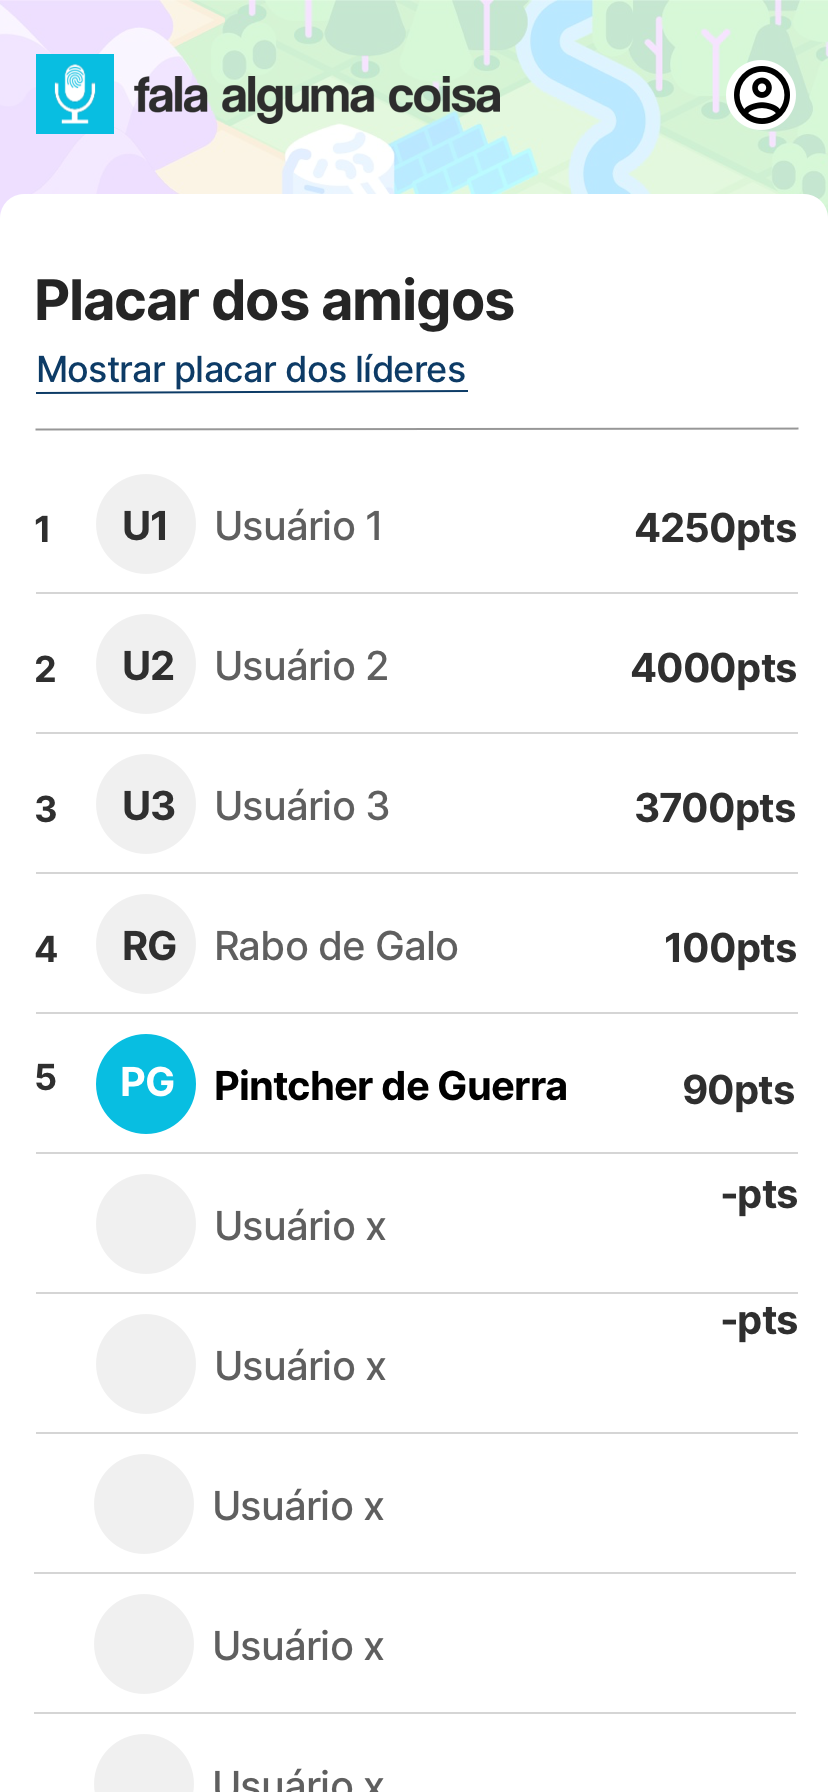
\includegraphics[width=.9\linewidth]{images/app/leaderboard/FriendsRanking.png}
      \caption{Friends Leaderboard}
      \label{fig:falealgumacoisa-leaderboard-page-design-friend}
    \end{subfigure}
    \caption*{Source: Author}
    \label{fig:falealgumacoisa-leaderboard-page-design}
\end{figure}

\subsubsection{Login and Registration}

The login and registration pages include essential features to the application: the ability to identify the user and maintain a history of recordings.

\begin{figure}[ht]
    \centering
    \caption{Fale Alguma Coisa Login and Registration Page designs}
    \begin{subfigure}{.5\textwidth}
      \centering
      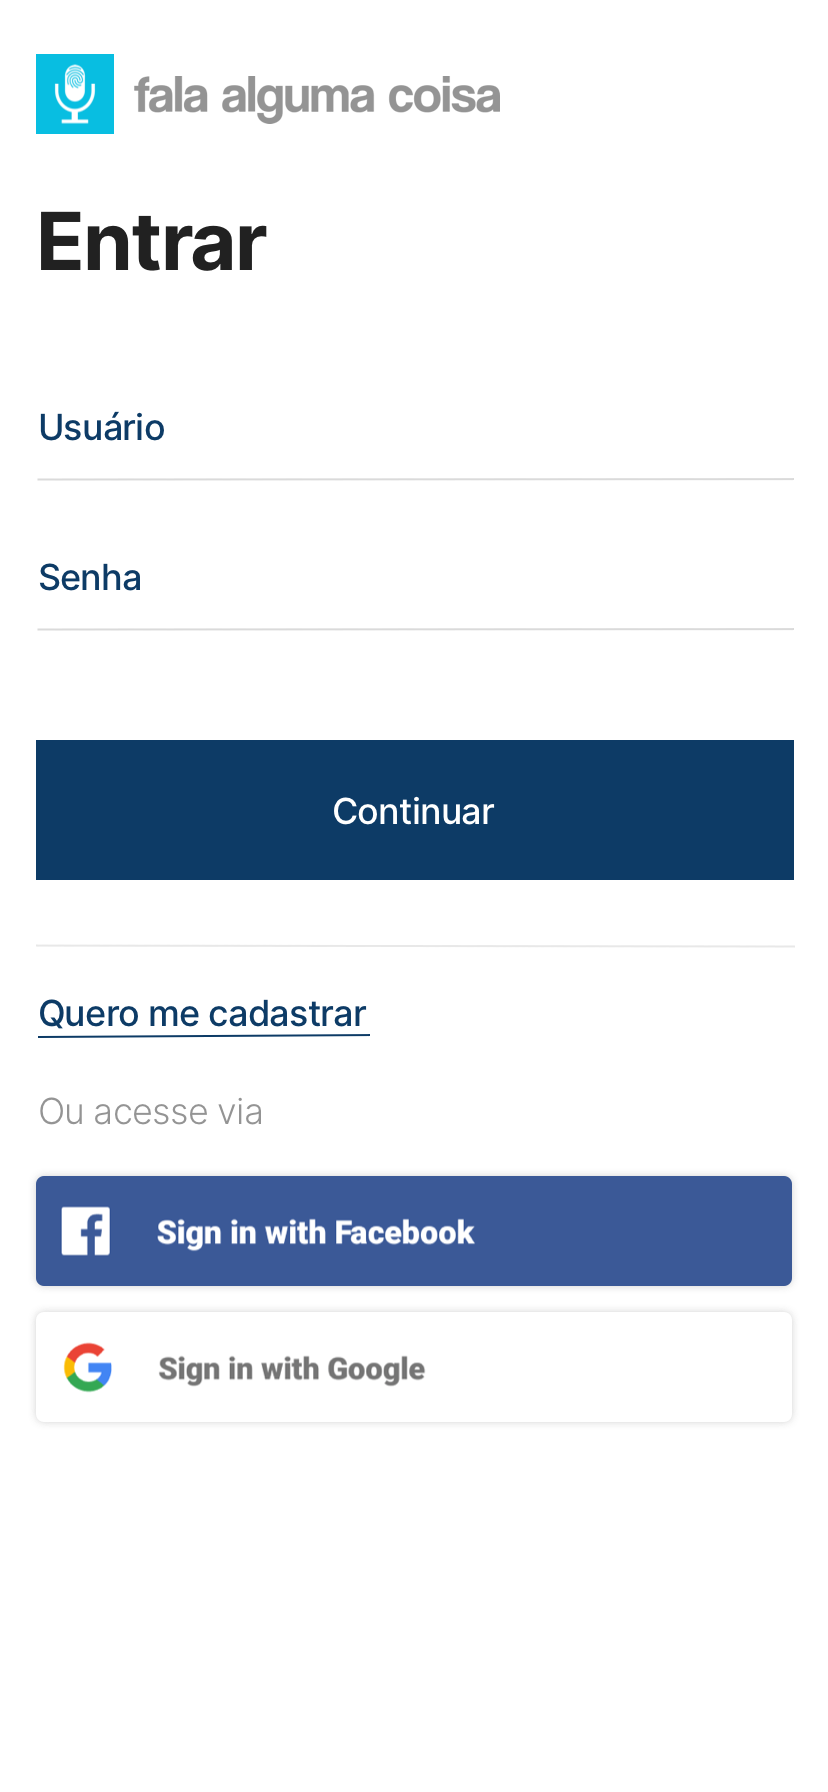
\includegraphics[width=.9\linewidth]{images/app/login/Login1.png}
      \caption{Login Page}
      \label{fig:falealgumacoisa-login-page-design}
    \end{subfigure}%
    \begin{subfigure}{.5\textwidth}
      \centering
      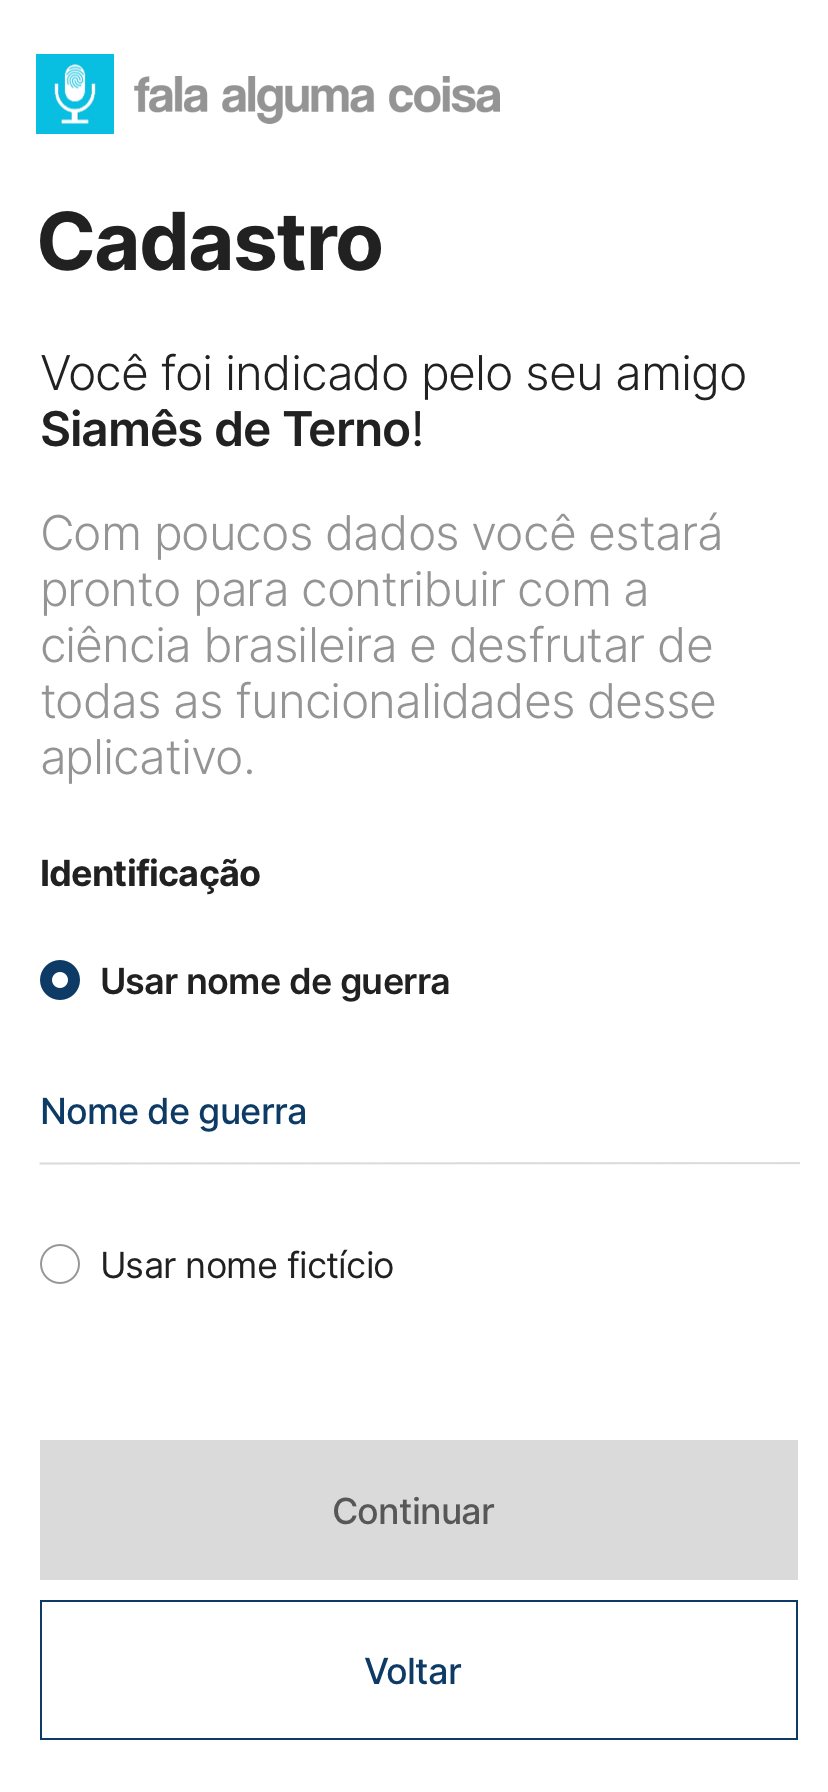
\includegraphics[width=.9\linewidth]{images/app/register/Register1.0.png}
      \caption{Registration Page}
      \label{fig:falealgumacoisa-registration-page-design}
    \end{subfigure}
    \caption*{Source: Author}
    \label{fig:falealgumacoisa-login-page-design}
\end{figure}

\subsubsection{Delete User}

If necessary, the user should be able to delete its user data, while still contributing his voice to the speech corpus. The following pages include the design of the layout for this deletion flow.

\begin{figure}[ht]
    \centering
    \caption{Fale Alguma Coisa Delete User Data Page design}
    \frame{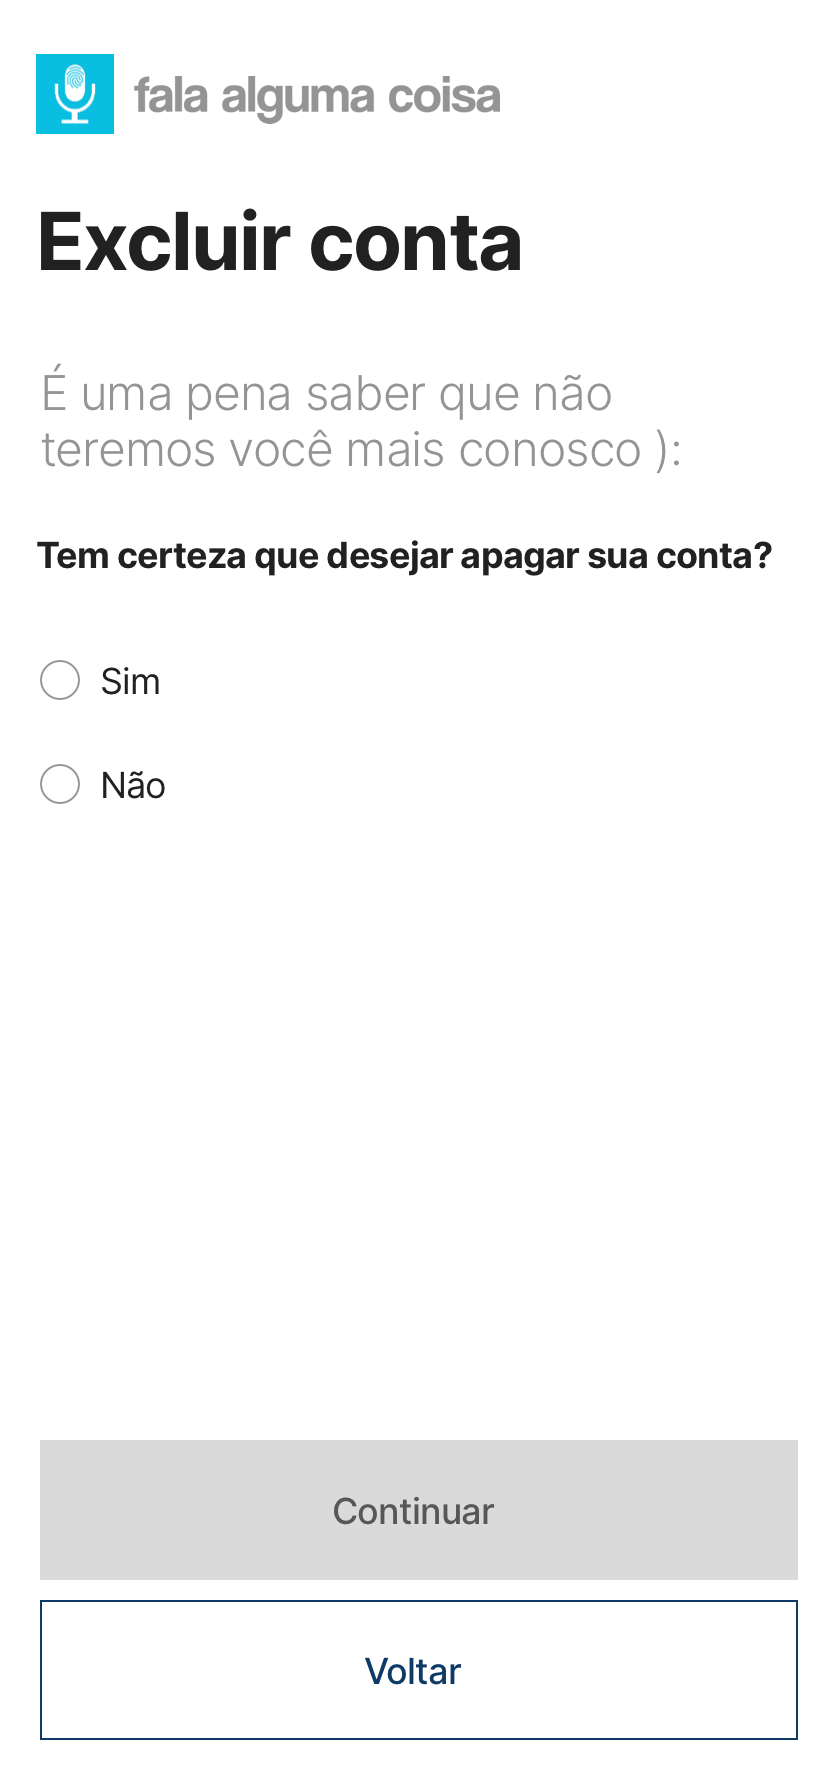
\includegraphics[width=\linewidth/2]{images/app/delete-user/FinishAccount1.0.png}}
    \caption*{Source: Author}
    \label{fig:falealgumacoisa-delete-user-data-page-design}
\end{figure}

\subsection{Development}

This section details the development process of the Fale Alguma Coisa app.

\subsubsection{Tools Selection}

To develop the application, a selection of tools was made. The table \ref{tab:tools-selection} details the selected tools and explains each choice.

\begin{table}[h]
    \centering
    \begin{tabular}{|c|c|c|}
        \hline Category & Selection & Explanation \\
        \hline Design & Zeplin & Easy sharing  \\ 
        \hline Desig &  & access \\ 
        \hline Galaxy Zoo & access & access \\ 
        \hline Christmas Audubom Birdwatch & access & access \\ \hline 
    \end{tabular}
    \caption{Contribution for online citizen science projects}
    \label{tab:cs-contributions}
\end{table}


\section{General Public Submission}
\label{sec:proposal-public-submission}

\section{Data Analysis}
\label{sec:proposal-data-analysis}

\section{Data Publication}
\label{sec:proposal-data-publication}
	\chapter{Application}
\label{chap:proposal-application}

This section details the conception, documentation, and development process of the voice recording application, coined "Fale Alguma Coisa". Below, it will at times be referenced as "app", or "WebApp", short for Application and Web Application, respectively. The main purpose of this app is to be able to record predetermined phrases from users. All other features support the engagement and usability through authentication, gamification, and explanatory elements. The following documentation structure is based on Pressman's book "Software Engineering: A Practitioner's Approach" \cite{pressman2014software}, and generated a proper Software Requirements Specification in the Appendix \ref{appendix:srs}. Hence, some details will be omitted to provide simplicity and overall understanding of the design process.

In this simplified explanation, the scope will be detailed \ref{sec:app-scope}, followed by the artefacts produced \ref{sec:app-artefacts}. Secondly, the functionality of the entire application will be documented using use cases (\ref{sec:simplified-use-cases}). Next, the navigation structure of some use cases will be documented (\ref{sec:navigation-design}), followed by the aesthetic design (in \ref{sec:aesthetic-design}). Then, the user interface will be elaborated by documenting the layouts (in \ref{sec:app-user-interface}), based on the use cases listed and previous decisions. One key factor in the app is the ability to teach science facts and trivia, which entails the need of proper phrase selection methods. These methods will be explained in the section \ref{sec:app-phrase-selection}. Lastly, the development process will be described, with additional details on the tools selected (\ref{sec:app-development}). Again, many steps of the software design process were skipped in this proposal, but a thorough description can be referred to in Appendix \ref{appendix:srs}.

\begin{figure}[ht]
    \centering
    \caption{Fale Alguma Coisa app Logo}
     
\includegraphics[width=\linewidth/2]{images/app/logo.jpg}
    \caption*{Source: Author}
    \label{fig:falealgumacoisa-logo}
\end{figure}

\section{Scope}
\label{sec:app-scope}

Towards contributing \textbf{nonprofessional scientists}, the Fale Alguma Coisa app should provide an easy gateway for the user to contribute his voice while having fun and learning various science facts and curiosities.

Towards researching \textbf{scientists}, the Fale Alguma Coisa app should provide a database of anonymized voice recordings for scientists to extract and create a speech corpus.

Directed towards anyone interested in learning and contributing to science.

\section{Outside scope}

However, some elements are outside of the scope of this system. These elements are clarified in this section, as Fale Alguma Coisa should \textbf{not}:
\begin{itemize}
    \item allow for association of recording data and personal identification data (name, email);
    \item support internationalization in the WebApp;
    \item convert audio data into another format;
    \item support offline recording.
\end{itemize}

\section{Artefacts}
\label{sec:app-artefacts}

This table presents the artefacts to be produced, and their respective locations in this work.

\begin{table}[h]
\centering
\caption{Artefacts produced by the specification and their respective locations}
\label{tab:artifact-locations}
\begin{tabular}{|p{3.5cm}|p{2.5cm}|p{9cm}|}
    \hline 
    Artefact & Location & Description \\ \hline 
    Purpose & Appendix \ref{appendix:purpose} & Defines the purpose of the Software Requirements Specification documentation \\ \hline
    Scope & Appendix \ref{appendix:scope} & Artefacts, Objectives, Out of Scope \\ \hline
    System Overview & Appendix \ref{appendix:system-overview} & Project perspective, System Context, General Constraints, Assumptions and Dependencies \\ \hline
    Actor List & Appendix \ref{appendix:actor-list} & List of actors involved with the system \\ \hline 
    Simplified Requirements & Section \ref{sec-simplified-use-cases} & Simplified use cases \\ \hline
    Scenario-based Models & Appendix \ref{appendix:scenario-based-model} & Detailed use cases \\ \hline
    Class Models & Appendix \ref{appendix:domain-model} & Class diagrams to model the domain of the system, mapping relationship and collaboration \\ \hline
    Behavior Models & Appendix \ref{appendix:behavior-model} & State and sequence diagrams to fully document specific and more complex behavior \\ \hline
    Non-Function Requirements & Appendix \ref{appendix:non-fuctional-requirements} & i.e.: Usability, Performance, Security, Legal, Requirements, etc. \\ \hline
    Interface Requirements & Appendix \ref{appendix:interface-requirements} & Machine and External Systems interfaces \\ \hline
    Navigation Design & Appendix \ref{appendix:navigation-design} & Navigation Semantic Units \\ \hline
    User Interface Design & Appendix \ref{appendix:user-interface-design} & For each use case, a user interface will be developed and documented \\ \hline
    Application Architecture & Appendix \ref{appendix:architecture} & Before WebApp must have  \\ \hline
    Tools and Frameworks Selection & Appendix \ref{appendix:tools-selection} & To develop the documented application, a set of tools and frameworks shall be selected \\ \hline
    FaleAlgumaCoisa WebApp & Appendix \ref{appendix:webapp} & Description of developed web application \\ \hline
    FaleAlgumaCoisa Backend & Appendix \ref{appendix:backend} & Description of developed backend application \\ \hline
\end{tabular}
\caption*{Source: Author}
\end{table}

\clearpage
\section{Use Cases}
\label{sec:simplified-use-cases}

A simplified list of use cases is reproduced in the following tables (\ref{tab:falealgumacoisa-simplified-home}, \ref{tab:falealgumacoisa-simplified-recording}, \ref{tab:falealgumacoisa-simplified-dashboard}, \ref{tab:falealgumacoisa-simplified-social}, \ref{tab:falealgumacoisa-simplified-gamification}, \ref{tab:falealgumacoisa-simplified-login-and-registration}) below, separated by feature set. To a more complete specification, refer to section \ref{appendix:use-cases} in the Appendix.

\subsection{Home}

In table \ref{tab:falealgumacoisa-simplified-home}, use cases affecting the homepage are listed, such as the splash screen, project description, navigation, and terms of service.

\begin{table}[h]
\caption{Simplified Home Use Cases for the Fale Alguma Coisa WebApp}
\label{tab:falealgumacoisa-simplified-home}
\centering
\begin{tabular}{|p{1cm}|p{3cm}|p{10cm}|}
\hline
    Code & Use Case Name & Description \\ \hline
    UC01 & View Home Splash & An unregistered citizen wants to view an animated introductory screen (splash) when entering the application, so that he feels more inside a native app. \\ \hline
    UC02 & View Home Description & An unregistered citizen wants to check the initiative description, so that he understands more about the Fale Alguma Coisa citizen science project. \\ \hline
    UC03 & Navigate Home Login & A registered citizen wants to navigates from the homepage to the sign-in page, so that he logins (or register) to his account. \\ \hline
    UC04 & Navigate Home Recording & An unregistered citizen wants to easily navigate from the homepage to the recording page, so that he can contribute his voice. \\ \hline
    UC05 & Read Home Terms & An unregistered citizen wants to reads the terms of service (and privacy policy) of Fale Alguma Coisa, so that he understands better what the service has to offer and what kind of data will be recorded. \\ \hline
\end{tabular}
\caption*{Source: Author}
\end{table}

\clearpage
\subsection{Recording}

Represents the most important feature in the application, as the citizen will use it to record his voice. It also provides supporting features, such as skipping phrases and resuming the recording session. The list of simplified use cases is listed in table \ref{tab:falealgumacoisa-simplified-recording}; with the complete version available in Appendix \ref{appendix:scenario-based-model}

\begin{table}[h]
\caption{Simplified Recording Use Cases for the Fale Alguma Coisa WebApp}
\label{tab:falealgumacoisa-simplified-recording}
\centering
\begin{tabular}{|p{1cm}|p{3cm}|p{10cm}|}
\hline
    Code & Use Case Name & Description \\ \hline
    UC10 & Accept Terms & An unregistered citizen would like to view and accept the terms of service before recording, so that he understands how his data is being used. \\ \hline
    UC11 & Configure Microphone & An unregistered citizen would like to properly configure my microphone before recording, so that he can record without interruption. \\ \hline
    UC12 & Record Phrases & A citizen would like to read science phrases with definitions and curiosities, so that he learns about subjects as he is contributing. \\ \hline
    UC13 & Group Phrases & A citizen would like to read phrases grouped by theme, so that he can learn more from each subject as he is contributing. To finish a theme, the citizen must read 6 phrases. \\ \hline
    UC14 & Read Tutorial & A citizen would like to read a tutorial explaining how to record, so that he learns how to properly record phrases. \\ \hline
    UC15 & Watch Recording Animations & A citizen would like to see animations on each step of the recording (enter the page, start the recording, stop the recording), so that he feels more engaged with the application. \\ \hline
    UC16 & Skip Phrase & A citizen would like to skip a phrase when he (1) does not know how to pronounce, or (2) finds a foreign word, or (3) finds another specified reason, so that he only speaks the correct phrases. A maximum of 2 skips are allowed. \\ \hline
    UC17 & Stop Recording Session & A citizen would like to stop this recording session by clicking the logo and confirming the exit, so that he can resume it afterwards. \\ \hline
\end{tabular}
\caption*{Source: Author}
\end{table}

\clearpage
\subsection{Dashboard}

Table \ref{tab:falealgumacoisa-simplified-dashboard} lists all user stories related to the dashboard page, such as where the user will be able to choose themes to record, open the menu, check his level, etc.

\begin{table}[h]
\caption{Simplified Dashboard Use Cases for the Fale Alguma Coisa WebApp}
\label{tab:falealgumacoisa-simplified-dashboard}
\centering
\begin{tabular}{|p{1cm}|p{3cm}|p{10cm}|}
\hline
    Code & Use Case Name & Description \\ \hline
    US20 & Navigate Register & An unregistered citizen would like to easily register his data through a button click, so that he can enjoy all features of the logged area. \\ \hline
    US21 & View Actions & A registered citizen would like to see his actions in a dashboard after logging in, so that he can better contribute to the project. \\ \hline
    US22 & Recommend Themes & A registered citizen would like to see a list of recommended themes to speak, so that he can choose one from the list. \\ \hline
    US23 & View Progress Level & A registered citizen would like to view my progress level, so that he know how far have he  progressed in my contributions. \\ \hline
    US24 & Open Menu & A registered citizen would like to open the menu, so that he knows which are his possible actions in the app. \\ \hline
    US25 & View Notifications & A registered citizen would like to check notifications, so that he understands what happened while he was gone. \\ \hline
\end{tabular}
\caption*{Source: Author}
\end{table}

\subsection{Social}

To allow the social interaction with other users, the table \ref{tab:falealgumacoisa-simplified-social} lists social use cases to be added to the application. Not all social interaction is listed in this feature, as there are some elements in gamification, such as competition.

\begin{table}[h]
\caption{Simplified Social Use Cases for the Fale Alguma Coisa WebApp}
\label{tab:falealgumacoisa-simplified-social}
\centering
\begin{tabular}{|p{1cm}|p{3cm}|p{10cm}|}
\hline
    Code & Use Case Name & Description \\ \hline
    US30 & Add Friend & A registered citizen would like to add a friend, so that he can check them in the friends leaderboard afterwards. \\ \hline
    US31 & View Notifications & A registered citizen would like to check notifications, so that he can know what happened when he was away. \\ \hline
    US32 & Receive Notifications & A registered citizen would like to know when someone added him through notifications, so that he can add them back later. \\ \hline
    US33 & Refer Friends & A registered citizen would like to refer friends to the application, so that he can play with them afterwards. \\ \hline
\end{tabular}
\caption*{Source: Author}
\end{table}

\subsection{Gamification}

Table \ref{tab:falealgumacoisa-simplified-gamification} details the engagement component of the application. Elements such as leaderboards, points and levels are described. They add competition and a sense of progress to the user experience, supporting the core need of this system, which is phrase recording.

\begin{table}[h]
\caption{Simplified Gamification Use Cases for the Fale Alguma Coisa WebApp}
\label{tab:falealgumacoisa-simplified-gamification}
\centering
\begin{tabular}{|p{1cm}|p{3cm}|p{10cm}|}
\hline
    Code & Use Case Name & Description \\ \hline
    US40 & Earn First Recording & A registered citizen would like to get 100 points when he records his first phrase, so that he can engage better in the application. \\ \hline
    US41 & Earn First Theme & A registered citizen would like to get 400 points when he records his first theme, so that he can engage better in the application. \\ \hline
    US42 & Earn Theme & A registered citizen would like to get 300 points when he records subsequent themes, so that he can engage better in the application. \\ \hline
    US43 & Earn Registration & A registered citizen would like to get 500 points when he registers his speaker data, so that he can better engage with the application. \\ \hline
    US44 & Calculate Level & A registered citizen would like to measure his points through a level, so that he can more easily compare himself with other users. \\ \hline
    US45 & Compete Top Players & A registered citizen would like to know who are the top contributors in the space and where he is in the list, so that he can compete against them. \\ \hline
    US46 & Compete Friends & A registered citizen would like to know where his friends are in the friends leaderboard, so that he can compete against them. \\ \hline
\end{tabular}
\caption*{Source: Author}
\end{table}

\subsection{Login and Registration}

The application should provide user authentication to enable data management and progress saving. Table \ref{tab:falealgumacoisa-simplified-login-and-registration} lists all use cases referring to this feature, and is the key to generating recordings with speaker metadata.

\begin{table}[h]
\caption{User Stories categorized to the login and registration epic for the Fale Alguma Coisa WebApp}
\label{tab:falealgumacoisa-simplified-login-and-registration}
\centering
\begin{tabular}{|p{1cm}|p{3cm}|p{10cm}|}
\hline
    Code & Use Case Name & Description \\ \hline
    US50 & Login Social & An unregistered citizen would like to login (using social login - Facebook / Google) on the app, so that he can login later and save my progress. \\ \hline
    US51 & Register Metadata & A unregistered citizen would like to register his anonymous data on his first login, so that he can provide better metadata to my recordings afterwards. \\ \hline
    US52 & Update Account & A registered citizen would like to update his account data, so that he can provide accurate metadata on the recordings. \\ \hline
    US53 & Delete Account & A registered citizen would like to remove his account data (and his recordings, if necessary), so that he can remove my metadata from this application. \\ \hline
\end{tabular}
\caption*{Source: Author}
\end{table}

\clearpage
\section{Navigation Design}
\label{sec:navigation-design}

Ensuring a robust navigation design for the user enables him to access the WebApp contents and functions. To accomplish this, it is necessary to: (1) identify the semantics of navigation for different users, and (2) define the mechanics of achieving the navigation. They are defined by a series of \textit{navigation semantic units} (NSUs), a set of information and related navigation structures that collaborate in the fulfillment of a subset of related user requirements \cite{conallen2003building}.

\subsection{Navigational Semantics}

A NSU is composed of a set of navigation elements called \textit{ways of navigating} (WoN). A WoN represents the the best navigation pathway to achieve a navigational goal for a specific type of user. Each WoN is organized as a set of \textit{navigational nodes} (NN) that are connected by navigational links. An example of NSU is given below in figure \ref{fig:app-nsu-example}.

\begin{figure}[h]
    \centering
    \caption{Navigation Semantic Unit for an Unregistered User Recording}
    \label{fig:app-nsu-example}
    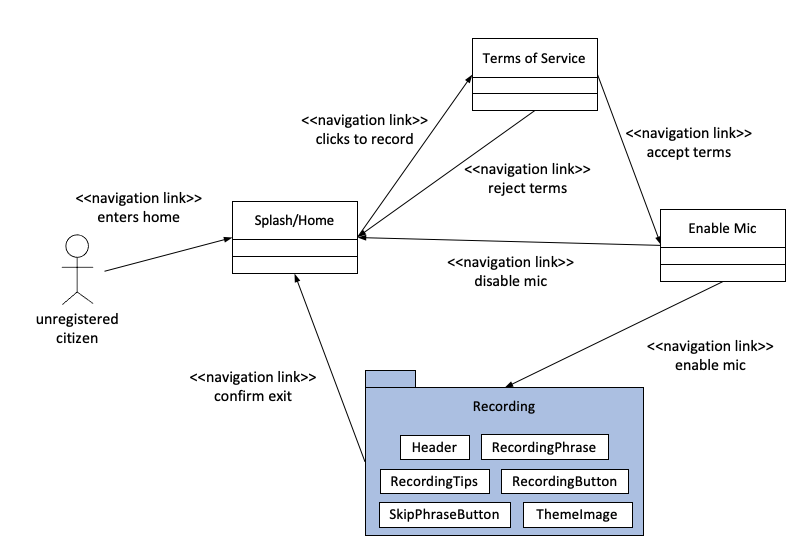
\includegraphics[width=\linewidth]{images/sw-req-spec/nsu-unregistered.png}
    \caption*{Source: Author}
\end{figure}

In figure \ref{fig:app-nsu-example}, the navigation behavior to record a phrase of an unregistered user is illustrated. As the unregistered user enters the homepage, he clicks the start recording button. However, since he has neither accepted the terms of service nor enabled his microphone permission, he must go through these pages. If he denies the terms or microphone permission, he is redirected to the homepage. If the user allows both, he will enter the recording page, where he is able to record phrases and donate his voice.

This is only one example of the more complex user Ways of Navigations. Refer to appendix \ref{appendix:navigation-design} to a more complete list of NSUs.

\section{Aesthetic Design}
\label{sec:aesthetic-design}

To reference some aesthetic design guidelines from \cite{pressman2014software}:

\begin{itemize}
    \item Emphasize content;
    \item Organize layout elements from top left to bottom right;
    \item Group navigation, content, and function geographically within the page;
    \item Do not extend your real state with the scrolling bar;
    \item Consider resolution and browser window size when designing layout.
\end{itemize}

\subsection{Color Scheme}

In color theory, colors are used to communicate meaning, but also affect mood, and perception \cite{agoston2013color}. The design color scheme defines a color palette to choose from when designing new visual elements. Applying this concept, a colorful color scheme was chosen to lighten the mood of the application, as shown in figure \ref{fig:falealgumacoisa-color-scheme}.

\begin{figure}[h]
    \centering
    \caption{Fale Alguma Coisa color scheme}
     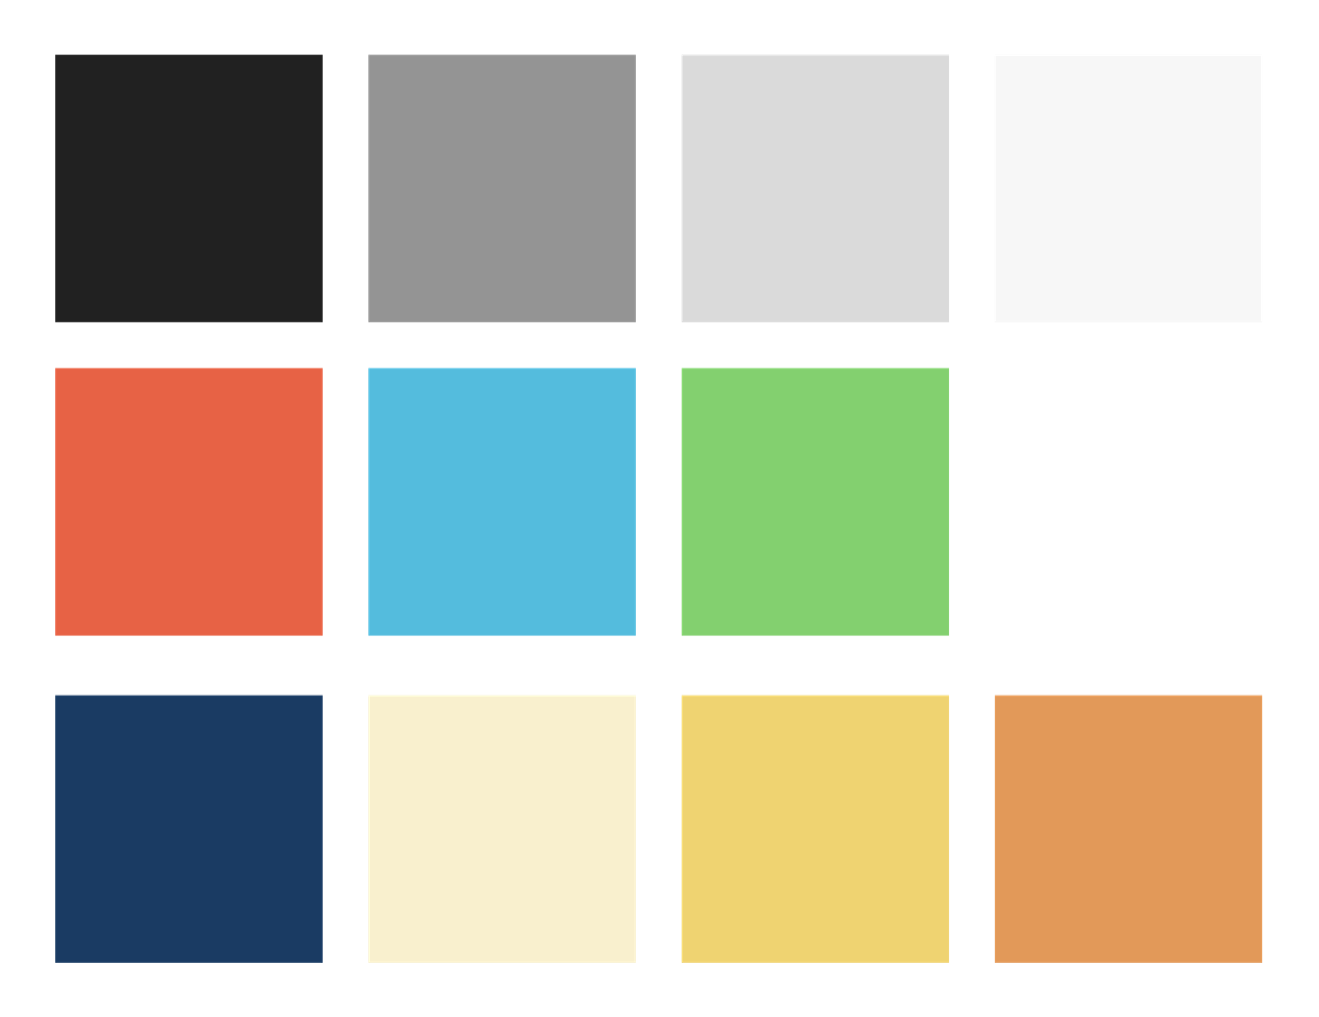
\includegraphics[width=.5\linewidth]{images/app/colors.png}
    \caption*{Source: Author}
    \label{fig:falealgumacoisa-color-scheme}
\end{figure}

\section{User Interface}
\label{sec:app-user-interface}

To ensure an effective development of the user interface, an iterative analysis and design approach was taken \cite{pressman2014software}. This design process is illustrated in figure \ref{fig:user-interface-design-process}, and emcompasses four distinct framework activities: (1) interface analysis and modeling, (2) interface design, (3) interface construction, and (4) interface validation. The spire implies that each of these tasks will occur more than once, with each pass around the spiral representing an additional elaboration of requirements and the resultant design. The user interface hereby implemented is the outcome of many of these iterations, with each major use case implemented into a finalized artefact. For an extensive list, refer to the Appendix \ref{appendix:user-interface-design}.

\begin{figure}[h]
    \centering
    \caption{The user interface design process}
    \label{fig:user-interface-design-process}
    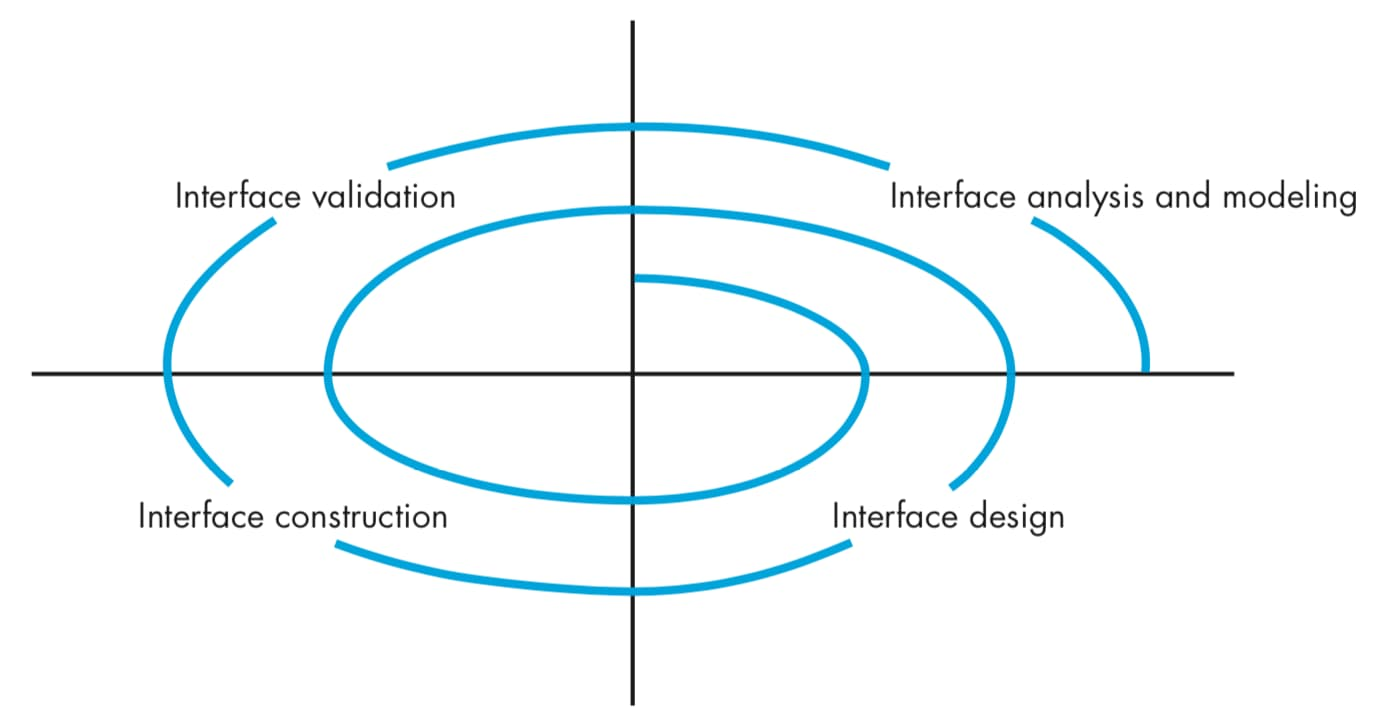
\includegraphics[width=.8\linewidth]{images/sw-req-spec/user-interface-design-process.jpg}
    \caption*{Source: \cite{pressman2014software}}
\end{figure}

\clearpage
\subsection{Splash and Home Screen}

As the user first enter the application, a splash screen will be shown to welcome him (mobile version in figure \ref{fig:falealgumacoisa-splash-page-design}). It contains the logo and an animation to draw the user's attention. After the animation, the home will be shown. After the splash animation, the homepage is shown. The mobile version can be seen below in figure \ref{fig:falealgumacoisa-home-page-design}. In this page, the call to action to start the recording is highlighted by the button at the center of the page, with text describing the project right below it. The login page is accessible through the link in the right upper corner. These few elements are placed to encourage the user to click on the recording, if he is a new user.

\begin{figure}[ht]
    \centering
    \caption{Fale Alguma Coisa Home Page designs}
    \begin{subfigure}{.5\textwidth}
      \centering
      \frame{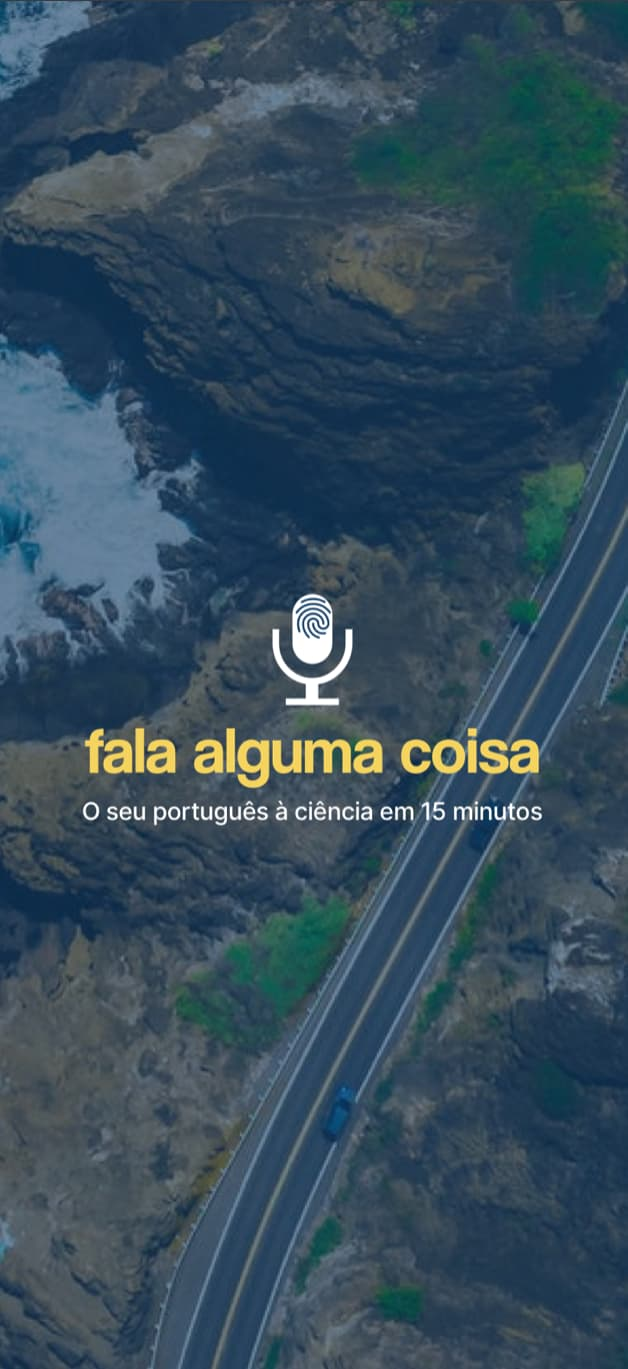
\includegraphics[width=.9\linewidth]{images/app/m-splash.jpg}}
      \caption{Fale Alguma Coisa Home Page design}
      \label{fig:falealgumacoisa-splash-page-design}
    \end{subfigure}%
    \begin{subfigure}{.5\textwidth}
      \centering
      \frame{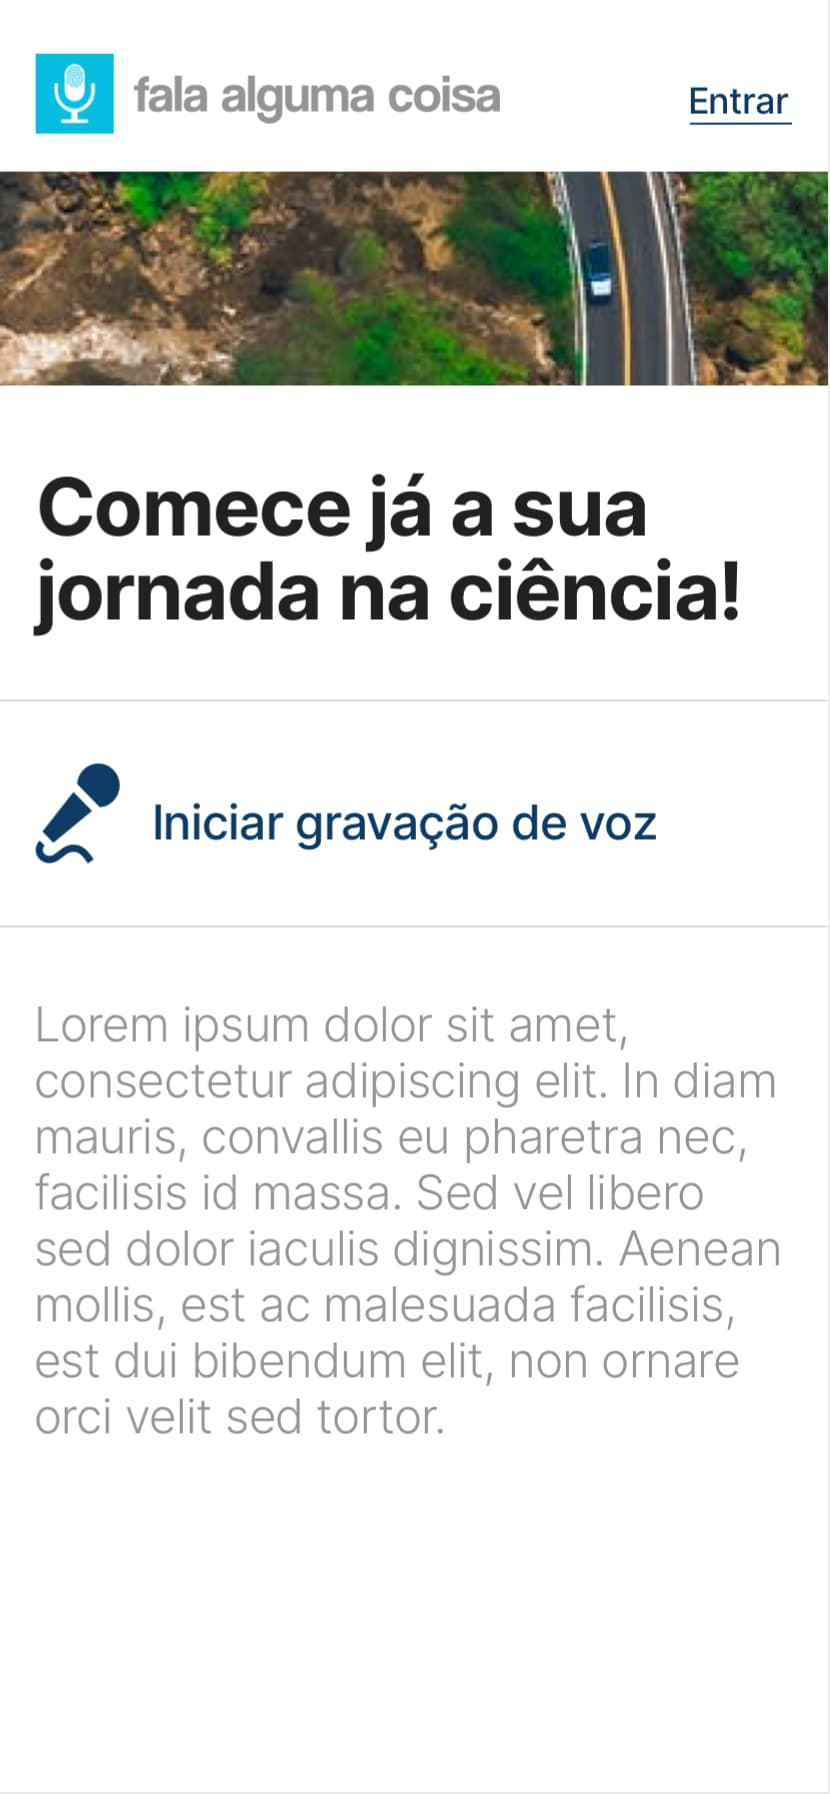
\includegraphics[width=.9\linewidth]{images/app/m-home.jpg}}
      \caption{Fale Alguma Coisa Home Page design}
      \label{fig:falealgumacoisa-home-page-design}
    \end{subfigure}
    \caption*{Source: Author}
    \label{fig:falealgumacoisa-home-page-designs}
\end{figure}

\subsection{Recording}

This page represents the core functionality of the website, allowing the user to record phrases with his voice. The recording is done through groups of phrases, called a theme, and is illustrated by the image \ref{fig:falealgumacoisa-recording-page-design} at the bottom. The main elements of the page are (1) the phrase highlighted in a rectangular box at the center of the page, and (2) the red recording button at the bottom.

\begin{figure}[ht]
    \centering
    \caption{Fale Alguma Coisa Recording Page designs}
    \begin{subfigure}{.5\textwidth}
      \centering
      \frame{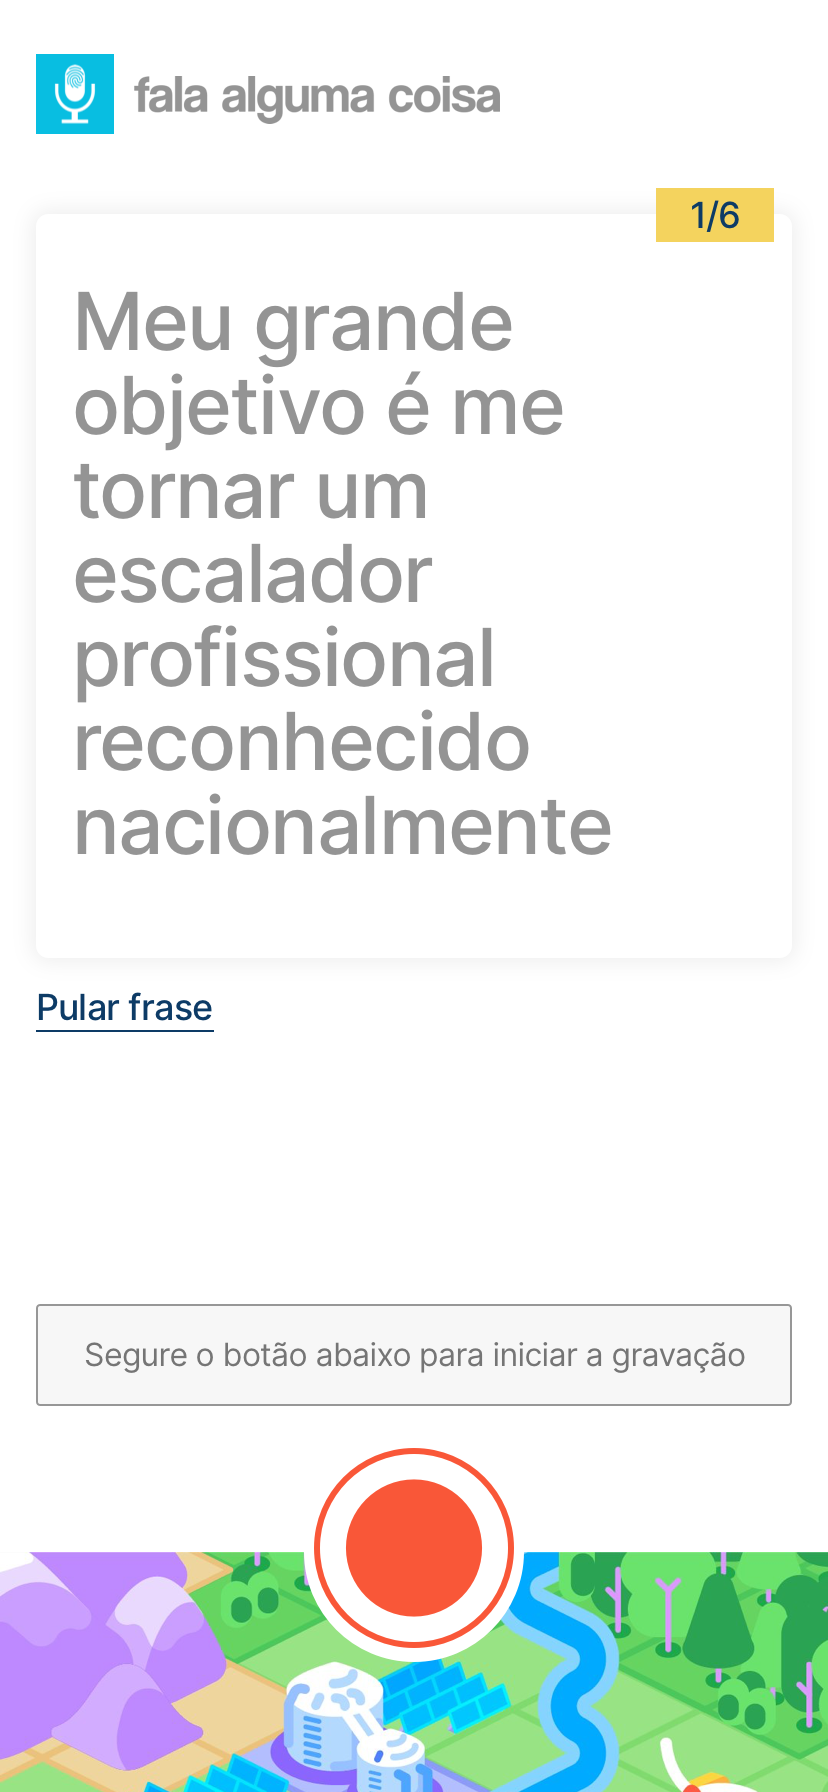
\includegraphics[width=.9\linewidth]{images/app/recording/Journey_1.0.png}}
      \caption{Waiting to start recording}
      \label{fig:falealgumacoisa-recording-page-design-start}
    \end{subfigure}%
    \begin{subfigure}{.5\textwidth}
      \centering
      \frame{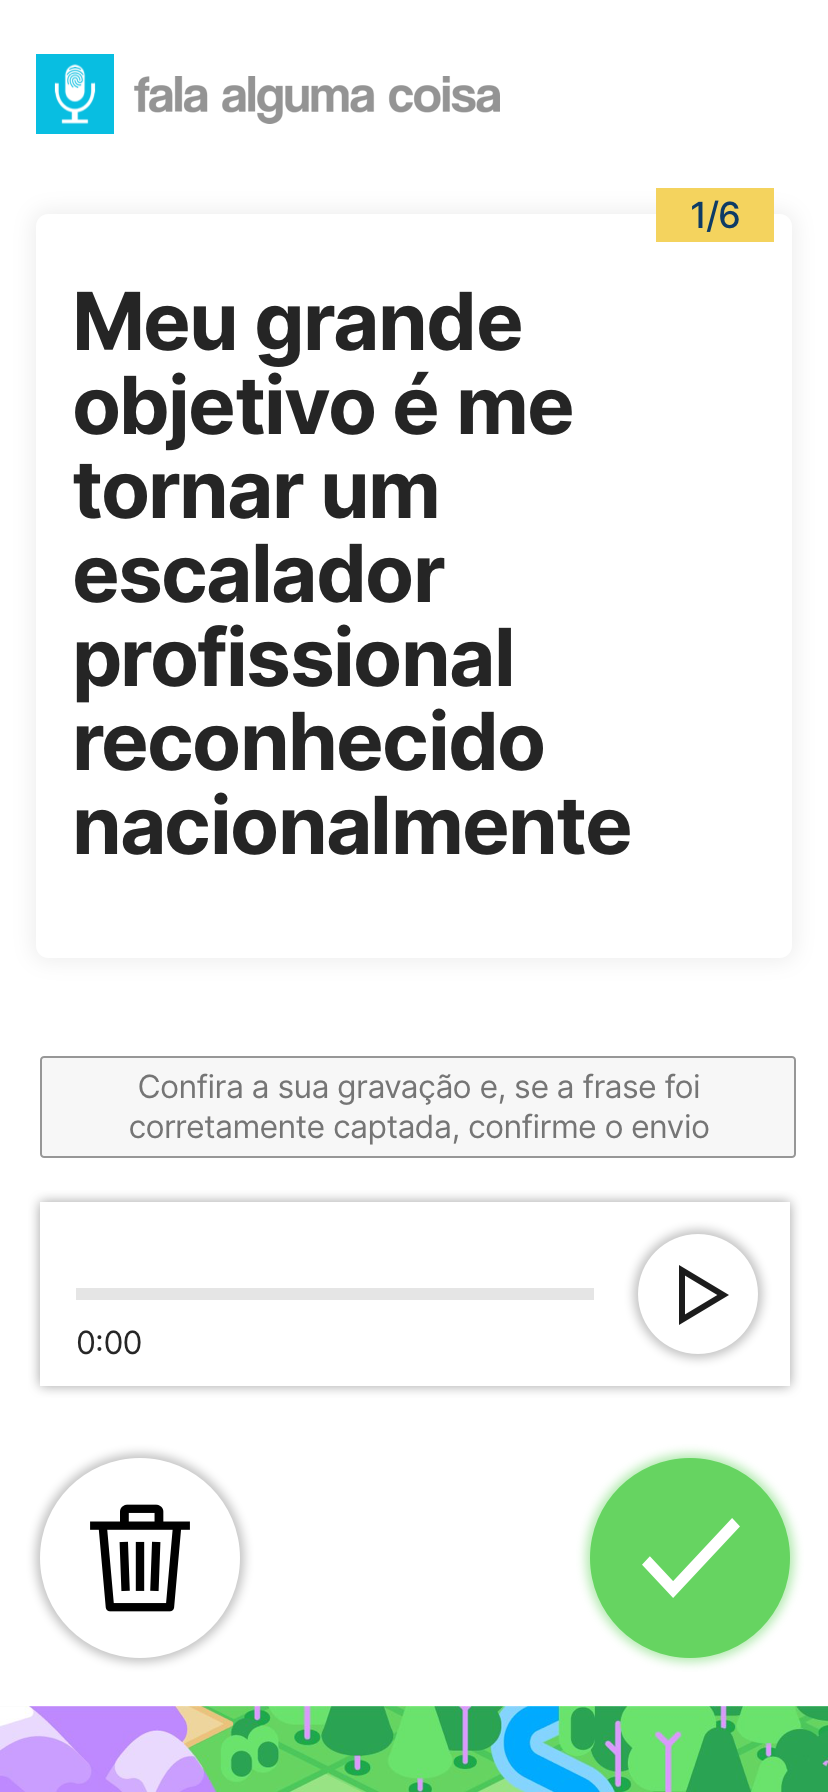
\includegraphics[width=.9\linewidth]{images/app/recording/Journey_1.2.png}}
      \caption{Confirm or delete recording}
      \label{fig:falealgumacoisa-recording-page-design-confirm}
    \end{subfigure}
    \caption*{Source: Author}
    \label{fig:falealgumacoisa-recording-page-design}
\end{figure}

\subsection{Terms of Service}

To comply with Brazil's General Data Protection Act (Law 13,709/2018), the application has to clarify the data usage of the visitor of the website. The layout just consists of text detailing the terms of service based on the law.

\subsection{Dashboard}

When an unauthenticated user finishes recording its first theme, or when a user logs in, they are able to select from a list of themes to record. In this dashboard seen in figure \ref{fig:falealgumacoisa-dashboard-page-design}, they are also shown the number of points accumulated by the usage of the app, as well as able to open a menu and notification page.

\begin{figure}[ht]
    \centering
    \caption{Fale Alguma Coisa Dashboard Page design}
    \frame{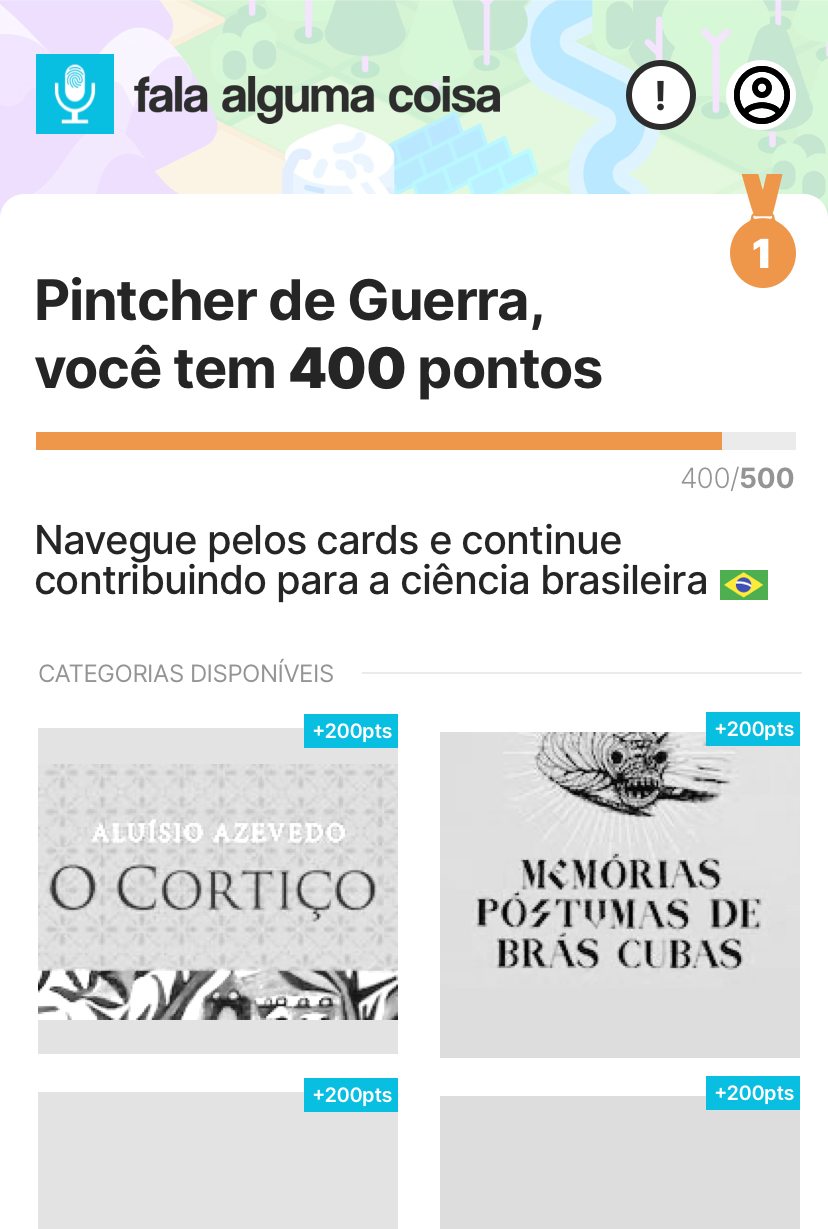
\includegraphics[width=\linewidth/2]{images/app/dashboard/DashboardCropped.png}}
    \caption*{Source: Author}
    \label{fig:falealgumacoisa-dashboard-page-design}
\end{figure}

\clearpage
\subsection{Leaderboard}

The leaderboard layouts feature two visualizations, depending on the desired scope. Should the contributor want to see all top ranking users, the leaderboard (figure \ref{fig:falealgumacoisa-leaderboard-page-design-general}) is available. If the user only wants to check his friend rankings, the application displays a reduced list (figure \ref{fig:falealgumacoisa-leaderboard-page-design-friend}), based on the friends added to the platform. These layouts provide a way for users to compare their contributions, thus promoting competition. A social element is also included throughout the option to add friends.

\begin{figure}[ht]
    \centering
    \caption{Fale Alguma Coisa Leaderboard Page designs}
    \begin{subfigure}{.5\textwidth}
      \centering
      \frame{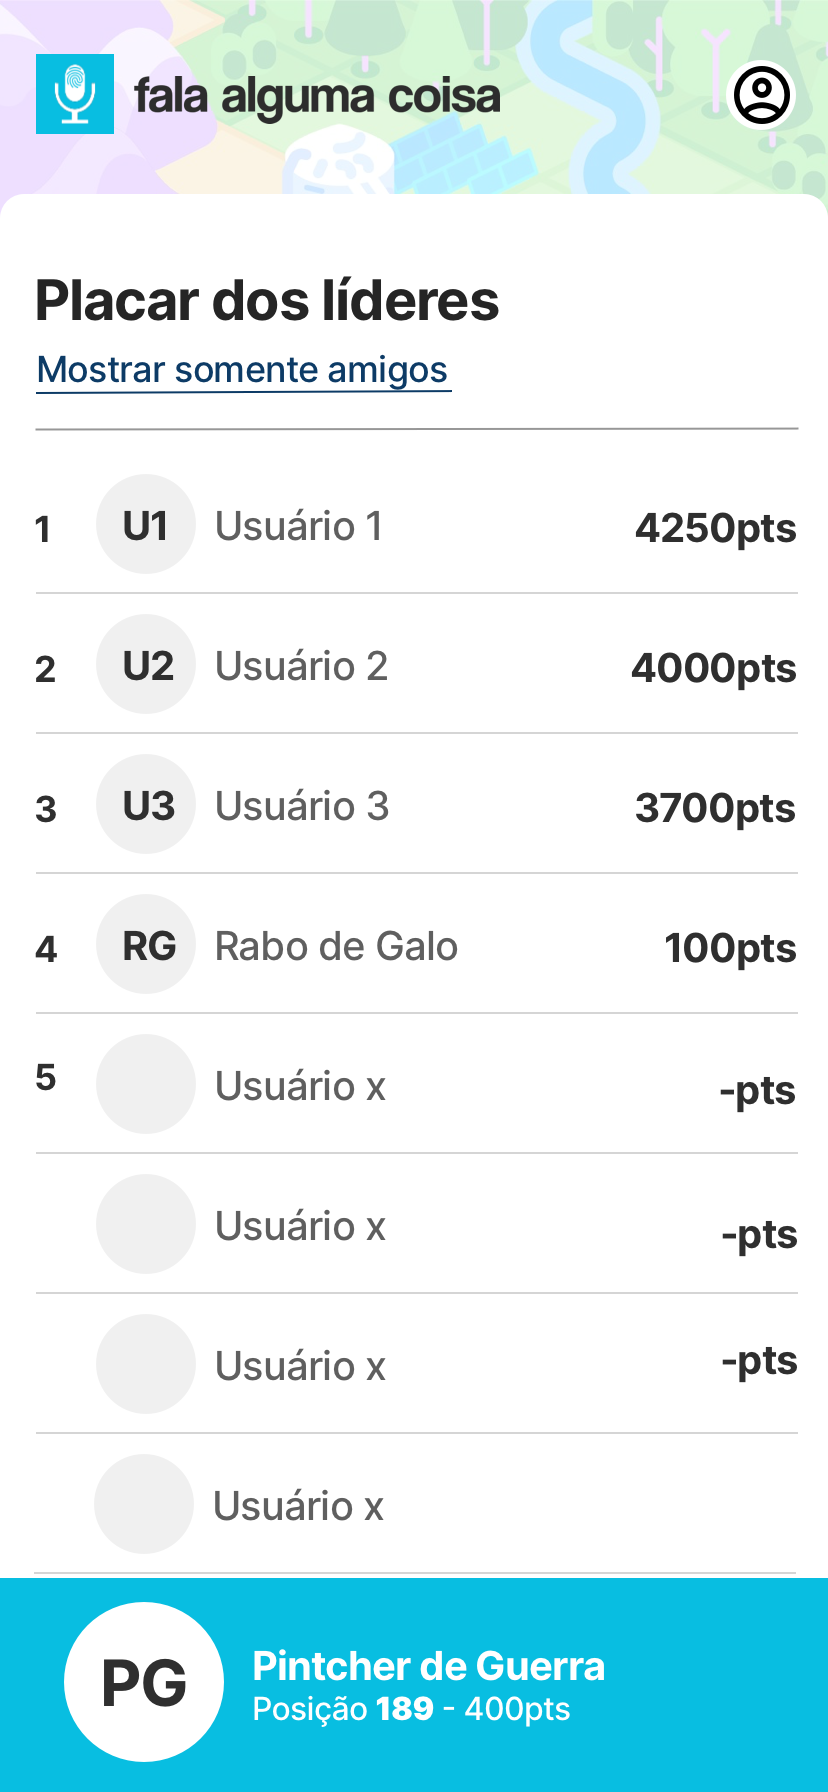
\includegraphics[width=.9\linewidth]{images/app/leaderboard/GeneralRanking.png}}
      \caption{General Leaderboard}
      \label{fig:falealgumacoisa-leaderboard-page-design-general}
    \end{subfigure}%
    \begin{subfigure}{.5\textwidth}
      \centering
      \frame{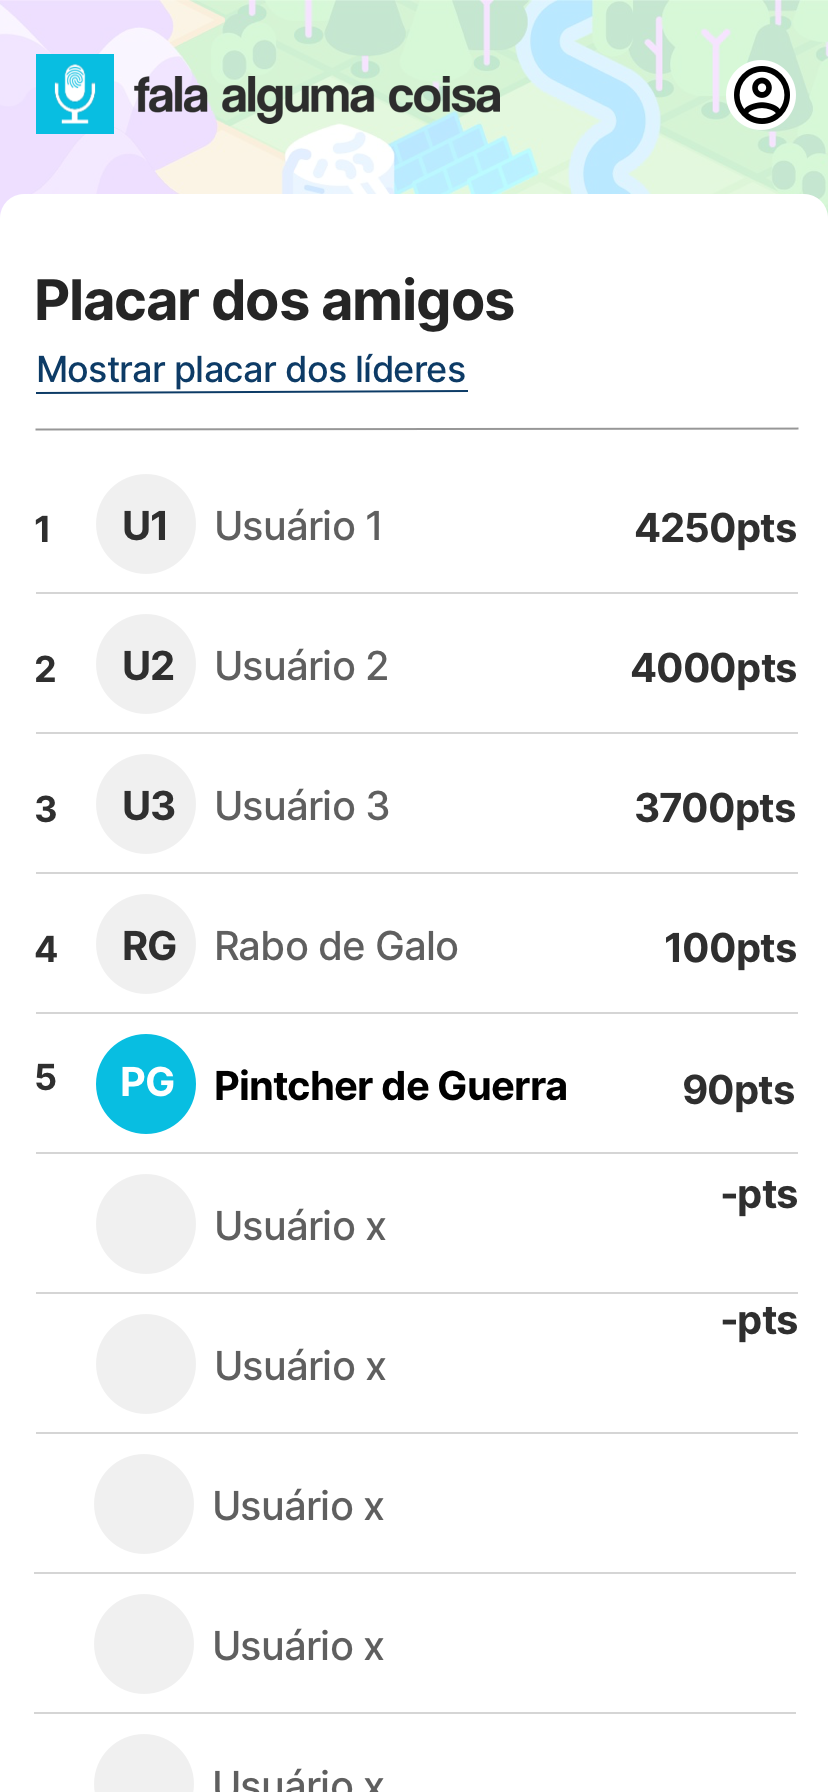
\includegraphics[width=.9\linewidth]{images/app/leaderboard/FriendsRanking.png}}
      \caption{Friends Leaderboard}
      \label{fig:falealgumacoisa-leaderboard-page-design-friend}
    \end{subfigure}
    \caption*{Source: Author}
    \label{fig:falealgumacoisa-leaderboard-page-design}
\end{figure}

\subsection{Friends}

The ability to add and track (follow) friends is possible with the layouts described below. If the contributor knows the nickname of his friend, he can search for his friends using the Search Friends page (seen in figure \ref{fig:falealgumacoisa-friends-page-design-search}). The results return in the same page below the search input field (figure \ref{fig:falealgumacoisa-friends-page-design-results}), as a list of users. To add a friend, it is as simple as clicking the "Seguir" button in the right corner of the result list. This click toggles the button with a "Seguindo" text. If this new state is clicked, the friend is removed.

\begin{figure}[h]
    \centering
    \caption{Fale Alguma Coisa Friends Page designs}
    \begin{subfigure}{.5\textwidth}
      \centering
      \frame{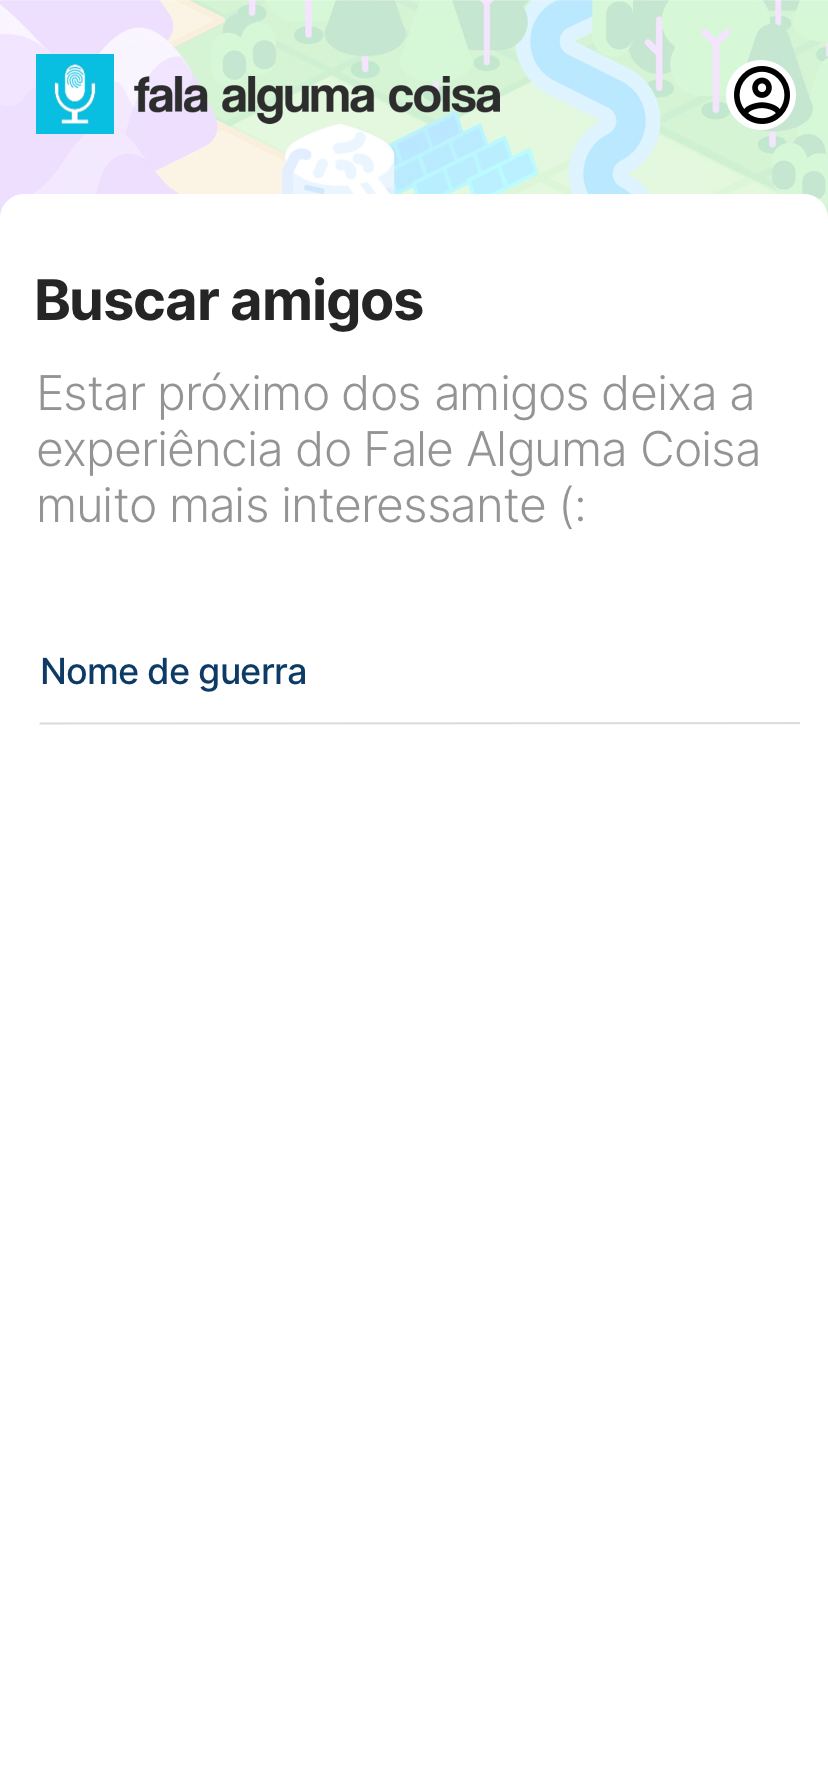
\includegraphics[width=.9\linewidth]{images/app/friends/FriendsSearch_1.0.png}}
      \caption{Search for friends}
      \label{fig:falealgumacoisa-friends-page-design-search}
    \end{subfigure}%
    \begin{subfigure}{.5\textwidth}
      \centering
      \frame{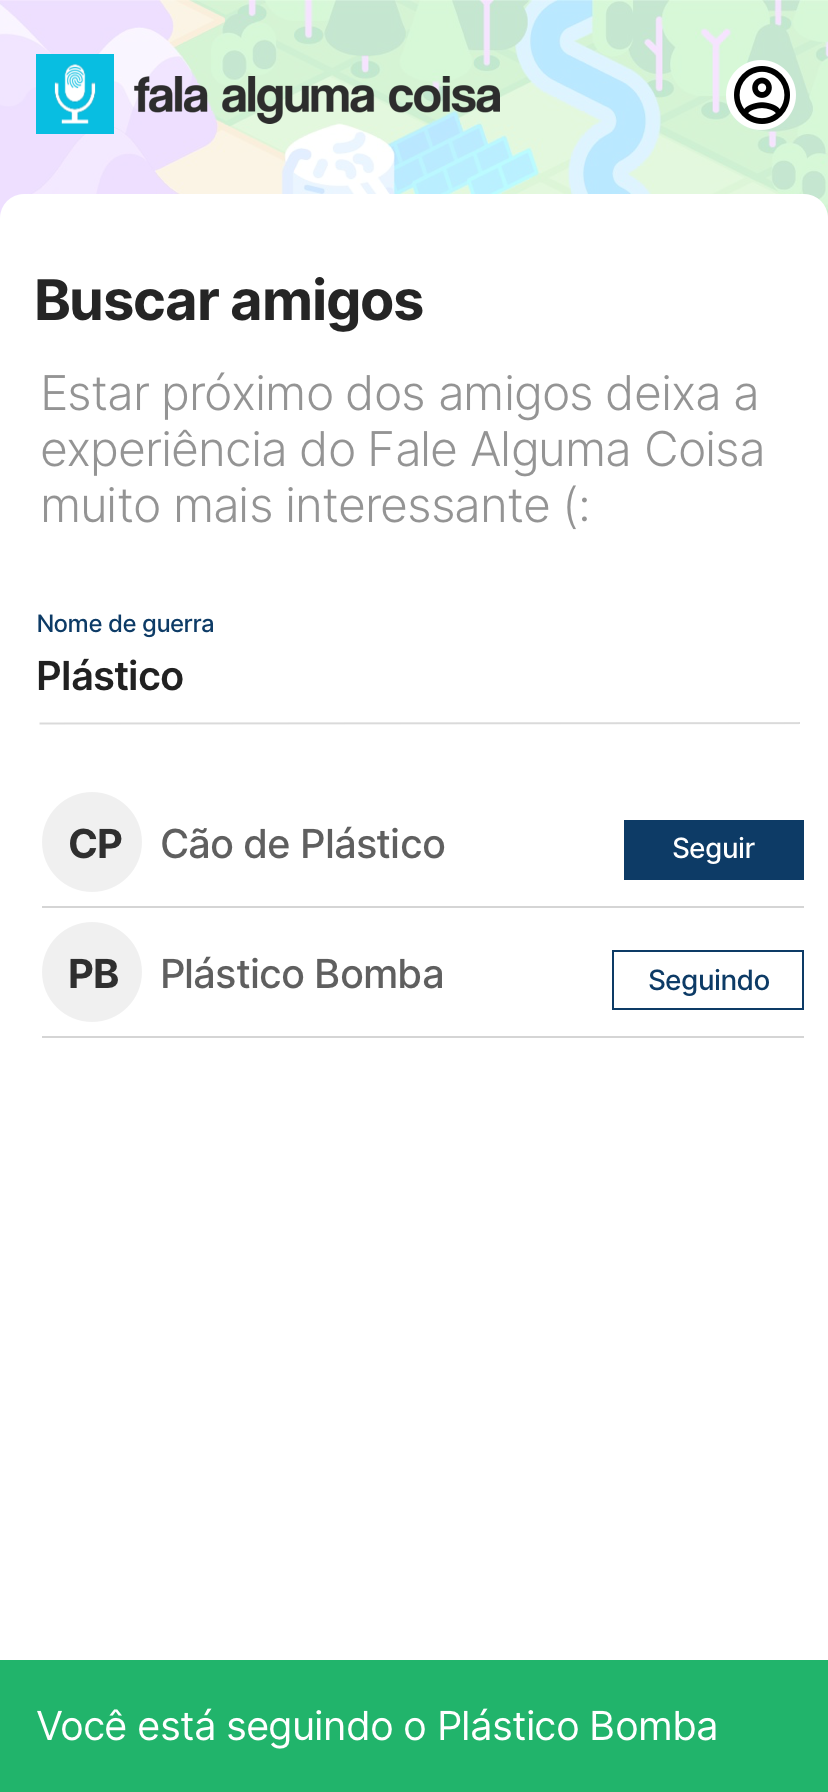
\includegraphics[width=.9\linewidth]{images/app/friends/FriendsSearch_1.3.png}}
      \caption{Search friends results}
      \label{fig:falealgumacoisa-friends-page-design-results}
    \end{subfigure}
    \caption*{Source: Author}
    \label{fig:falealgumacoisa-friends-page-design}
\end{figure}

\subsection{Refer Friends}

To earn more contribution points, the citizen scientist can also refer new friends using the Refer friends page. Clicking a button alows the user to share a like. The link shared redirects to a registration page, and both users get 100 points after the registration of the referred user. More details on \ref{appendix:sec:refer-a-friend}.

\subsection{Login and Registration}

The login and registration pages include essential features to the application: the ability to identify the user and maintain a history of recordings. The figure in \ref{fig:falealgumacoisa-login-page-design} represents a login flow possible to the contributor - using a username and password. It is also possible to use the "social login" through Facebook and Google, identifiable by the respective buttons in the layout.

\begin{figure}[h]
    \centering
    \caption{Fale Alguma Coisa Login Page designs}
    \begin{subfigure}{.5\textwidth}
      \centering
      \frame{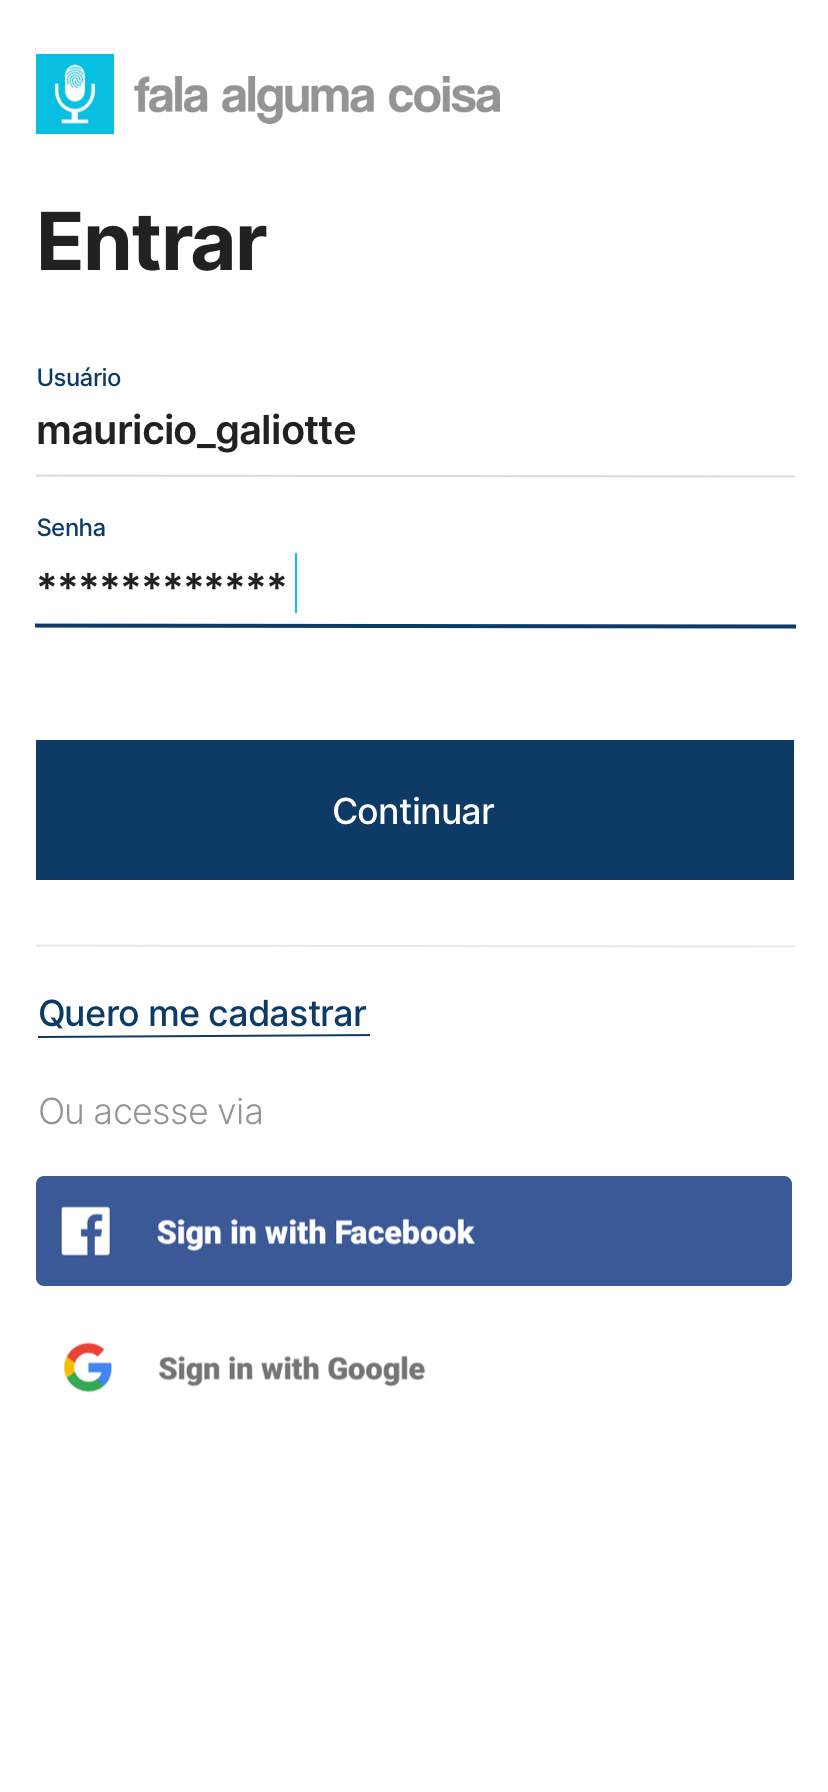
\includegraphics[width=.7\linewidth]{images/app/login/Login2.png}}
      \caption{Login with email and password}
      \label{fig:falealgumacoisa-login-page-design}
    \end{subfigure}%
    \begin{subfigure}{.5\textwidth}
      \centering
      \frame{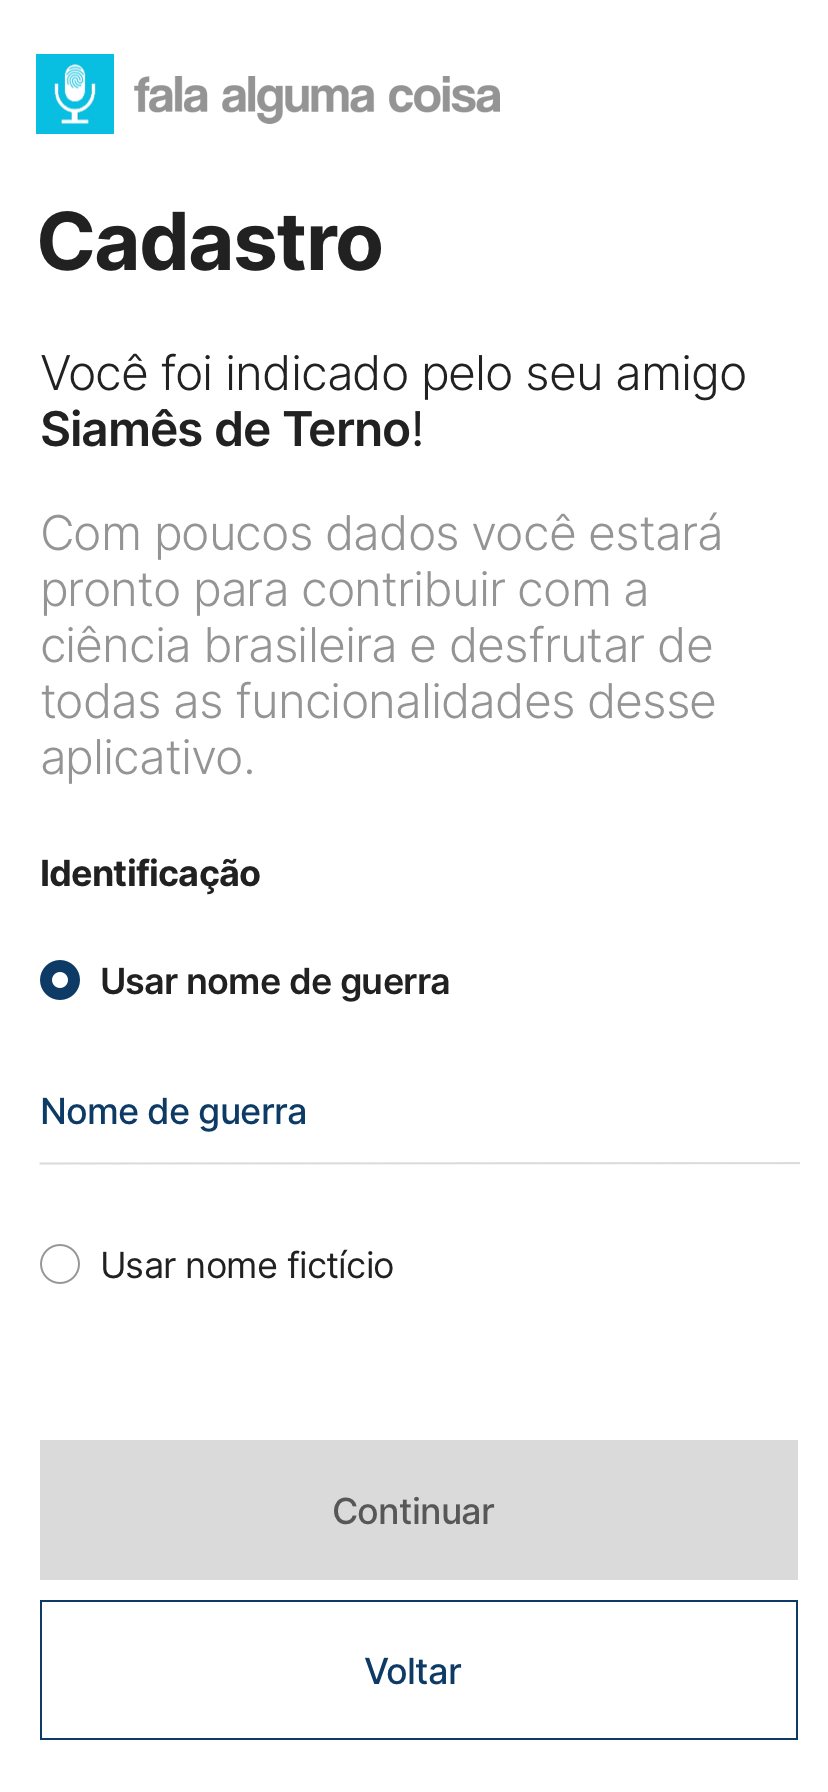
\includegraphics[width=.7\linewidth]{images/app/register/Register1.0.png}}
      \caption{Registration with \textit{pen name} selection}
      \label{fig:falealgumacoisa-registration-page-design-pen-name}
    \end{subfigure}
    \caption*{Source: Author}
    \label{fig:falealgumacoisa-login-and-registration-page-design}
\end{figure}

To register with the Fale Alguma Coisa app, the user must choose his \textit{pen name} (figure \ref{fig:falealgumacoisa-registration-page-design-pen-name}) and add some demographics information (seen in figure \ref{fig:falealgumacoisa-registration-page-design-demographics}. The registration flow can be triggered in two ways, and each have their differences:

\begin{itemize}
    \item Using the "social login" button. In this format, the user authenticates using the social media account and therefore does not need to provide email and password. Subsequent logins should use this method as well.
    \item Using a manual registration button ("Quero me cadastrar"). In addition to the name and demographics, the user must also provide his email and password as a last step (figure \ref{fig:falealgumacoisa-registration-page-design-email-password}).
\end{itemize}

\begin{figure}[h]
    \centering
    \caption{Fale Alguma Coisa Registration steps designs}
    \begin{subfigure}{.5\textwidth}
      \centering
      \frame{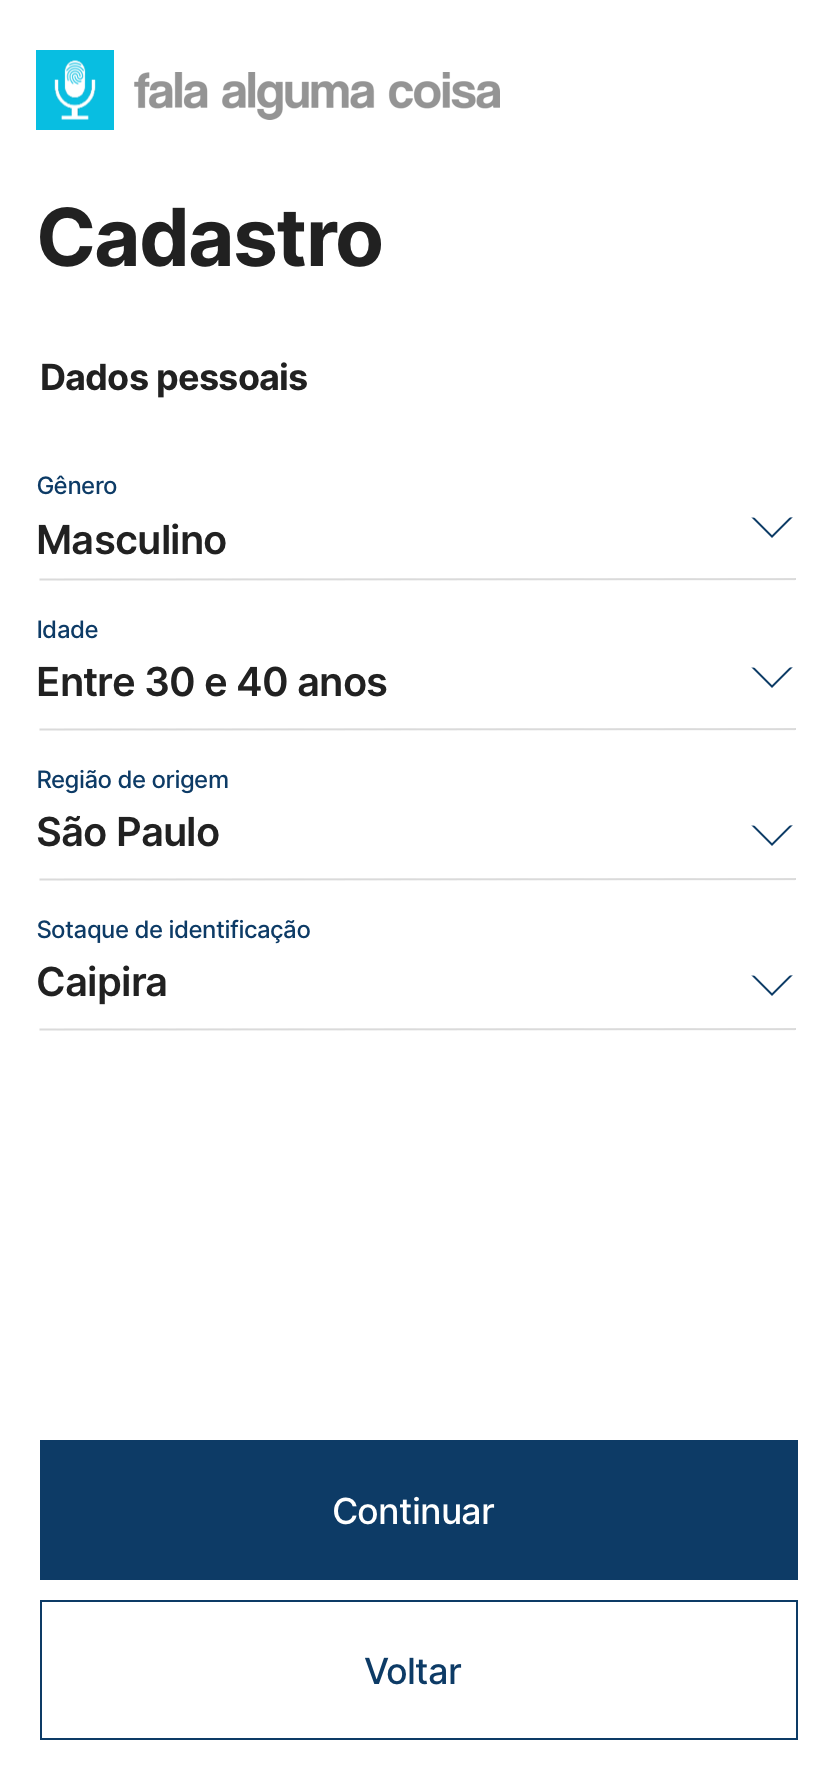
\includegraphics[width=.9\linewidth]{images/app/register/Register2.1.png}}
      \caption{Demographics step}
      \label{fig:falealgumacoisa-registration-page-design-demographics}
    \end{subfigure}%
    \begin{subfigure}{.5\textwidth}
      \centering
      \frame{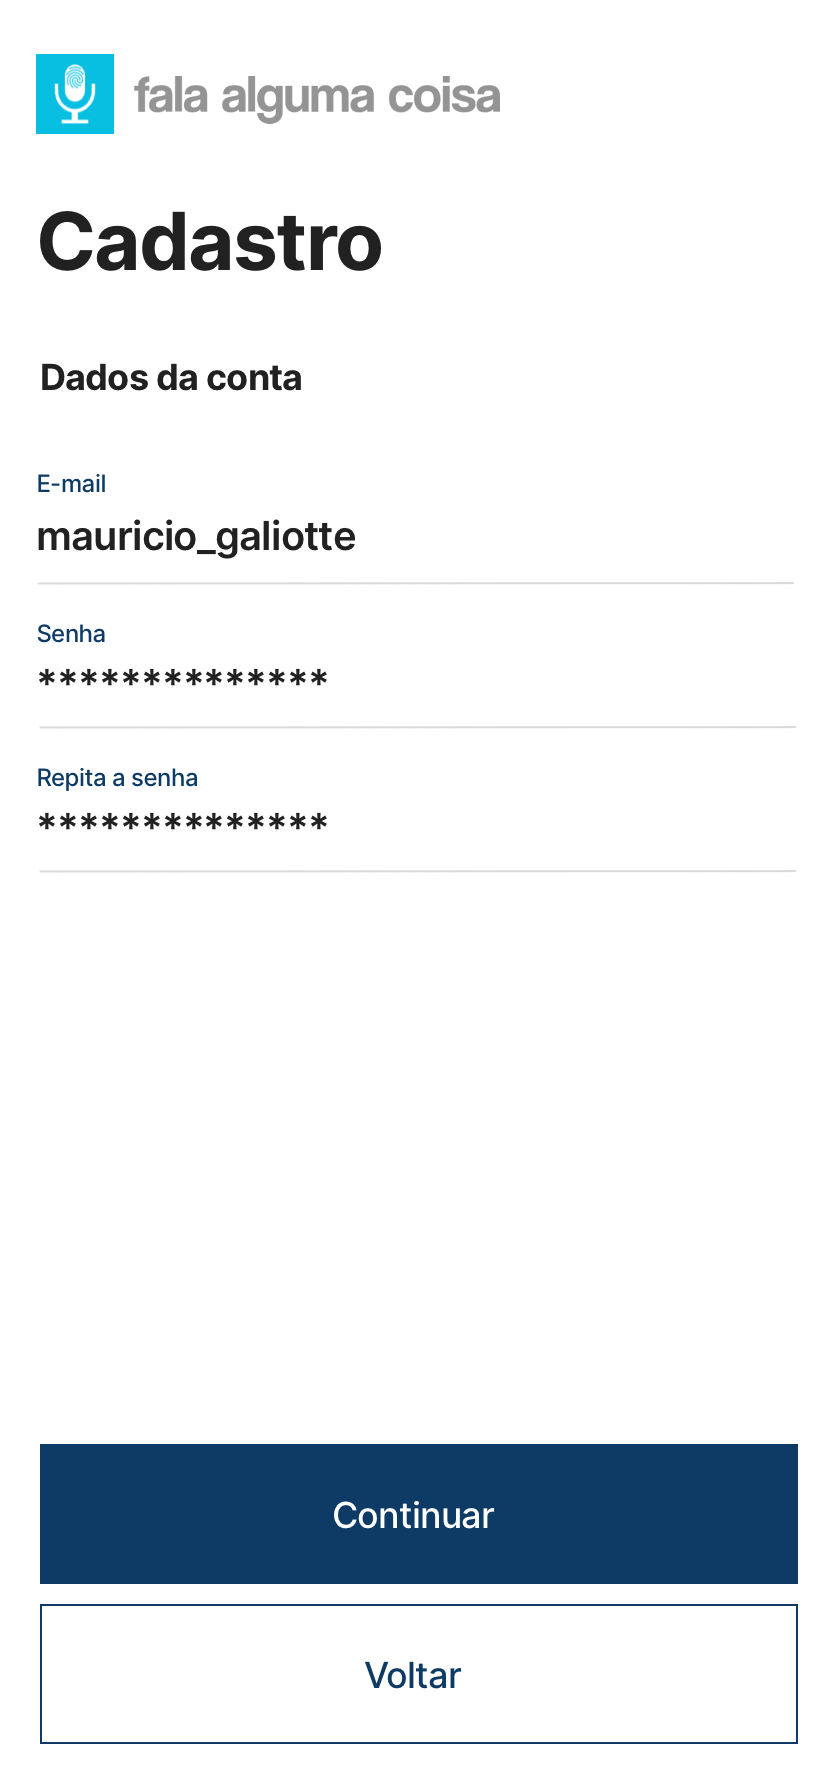
\includegraphics[width=.9\linewidth]{images/app/register/Register3.0.png}}
      \caption{Email and password step}
      \label{fig:falealgumacoisa-registration-page-design-email-password}
    \end{subfigure}
    \caption*{Source: Author}
    \label{fig:falealgumacoisa-registration-page-design}
\end{figure}

\subsection{Delete User}

If necessary, the user should be able to delete its user data, while still contributing his voice to the speech corpus. The following figures (\ref{fig:falealgumacoisa-delete-user-data-page-design-1} and \ref{fig:falealgumacoisa-delete-user-data-page-design-2}) include the design of the layout for this deletion flow.

\begin{figure}[h]
    \centering
    \caption{Fale Alguma Coisa Delete User Data steps designs}
    \begin{subfigure}{.5\textwidth}
      \centering
      \frame{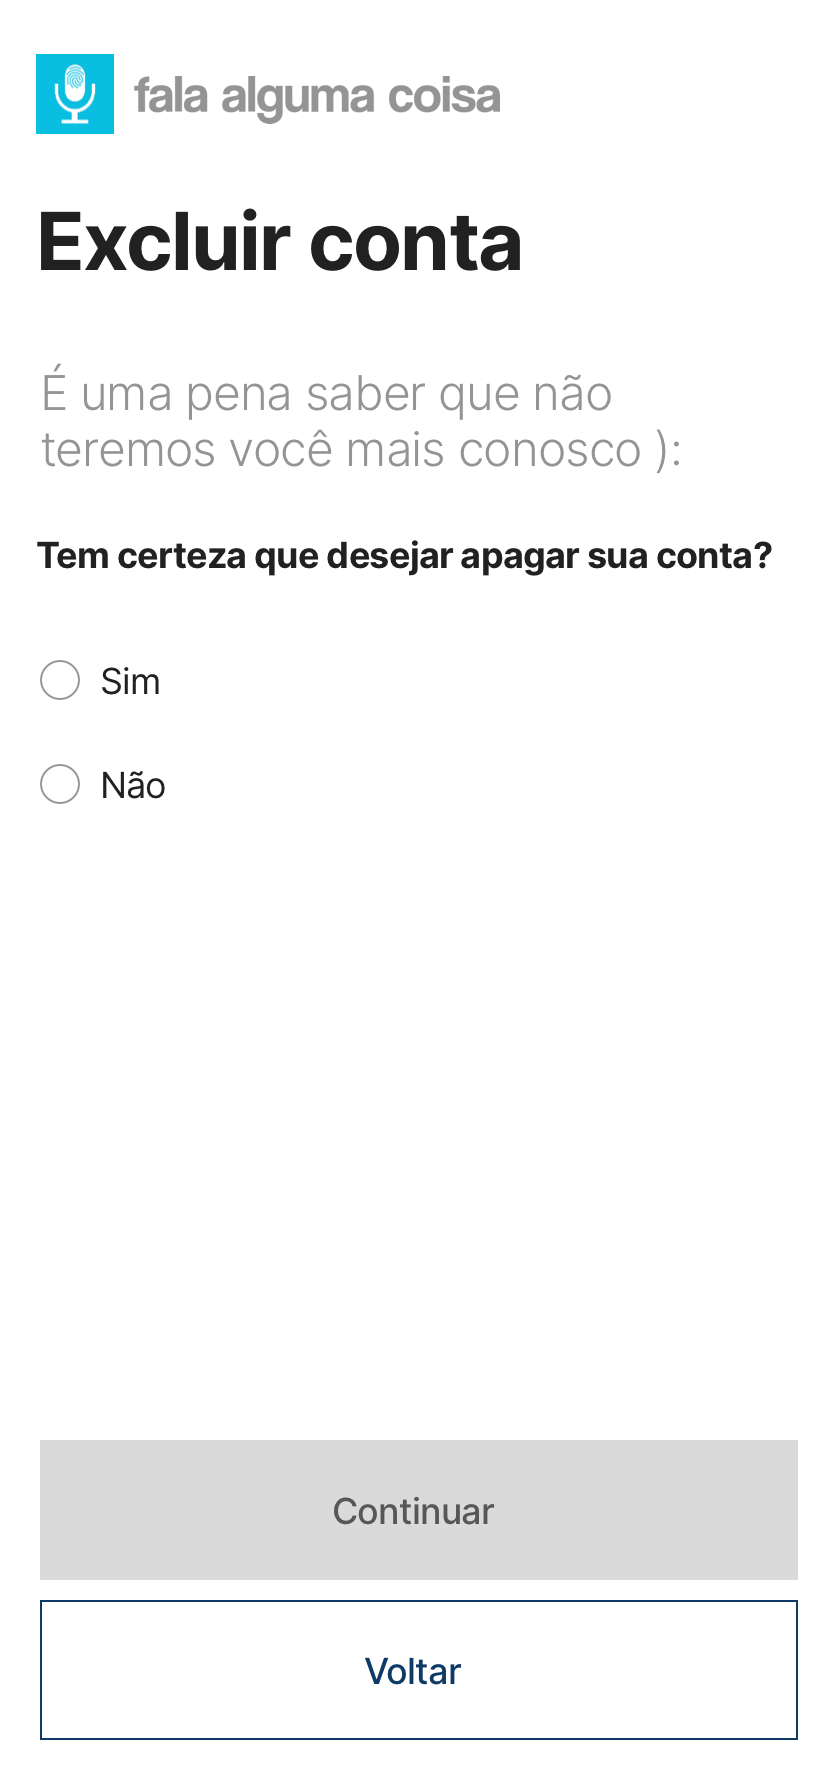
\includegraphics[width=.9\linewidth]{images/app/delete-user/FinishAccount1.0.png}}
      \caption{Deletion confirmation}
      \label{fig:falealgumacoisa-delete-user-data-page-design-1}
    \end{subfigure}%
    \begin{subfigure}{.5\textwidth}
      \centering
      \frame{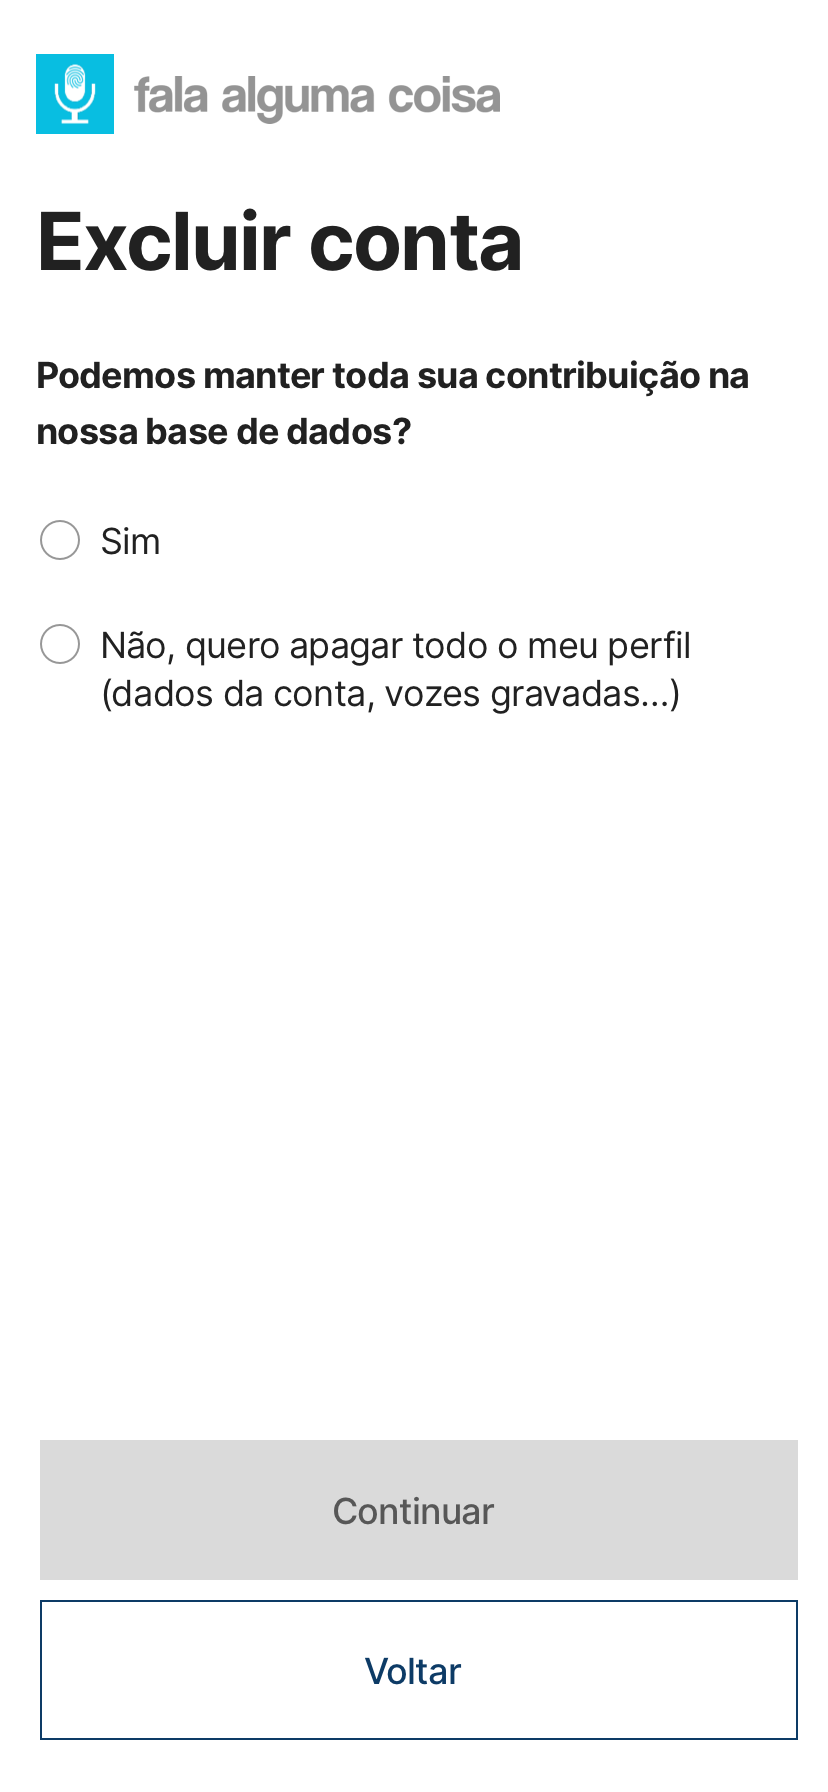
\includegraphics[width=.9\linewidth]{images/app/delete-user/FinishAccount2.0.png}}
      \caption{Scope of deletion}
      \label{fig:falealgumacoisa-delete-user-data-page-design-2}
    \end{subfigure}
    \caption*{Source: Author}
    \label{fig:falealgumacoisa-delete-user-data-page-design}
\end{figure}

\subsection{Remaining Implementations}

Refer to Appendix \ref{appendix:user-interface-design} for the remaining implemented user interfaces.

\clearpage
\section{Phrase Selection}
\label{sec:app-phrase-selection}

One of the key aspects of the Fale Alguma Coisa application is the ability of explaining science-related trivia. In the process of recording, the contributor may learn small facts about the chosen topic by reading a group of scientific phrases. The following sections will detail (1) the anatomy of a theme, (2) the requirements for selecting a phrase, (3) the source for an initial list of phrases, along with (4) the filtering process. Then, (5) images are selected for each theme, and lastly (5) the phrases and images are inputted to the application. 

Except for the last step of integrating with the application, this process is fully automated by a Jupyter Notebook in Python 3, and the complete source code is available on GitHub at \url{https://github.com/gabrieltnishimura/cv-sentence-extractor}.

\subsection{Theme Anatomy}

Each group of phrases is entitled "theme". By specification (\ref{srs:uc12} and \ref{srs:uc16}), a theme is composed of 8 phrases, 6 of which must be recorded to finish a theme; allowing up to 2 skips. Figure \ref{fig:falealgumacoisa-phrase-all} illustrates this structure and figure \ref{phrase-skip} displays what happens to a recording group when a phrase is skipped.

\begin{figure}[h]
    \centering
    \caption{Selected phrases of a theme. Out of 8, only 6 are shown to the user.}
    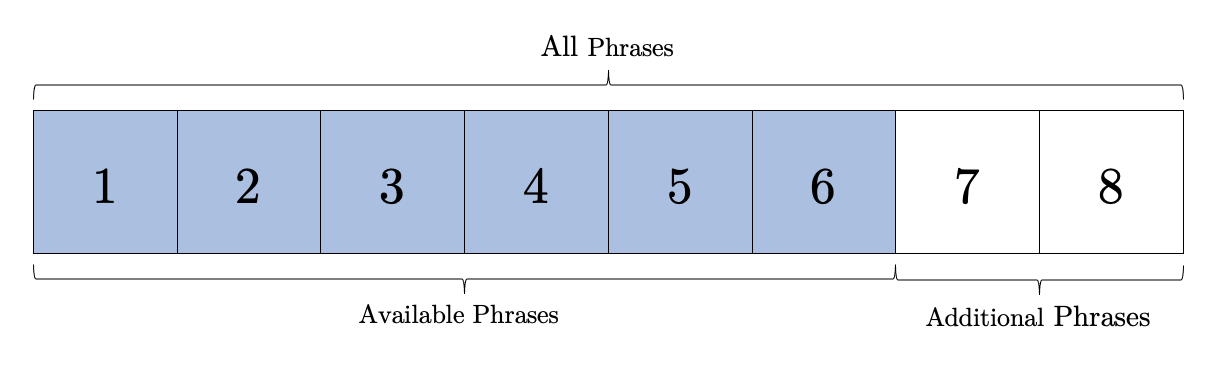
\includegraphics[width=\linewidth]{images/phrase-selection/phrase-all.png}
    \caption*{Source: Author}
    \label{fig:falealgumacoisa-phrase-all}
\end{figure}

\begin{figure}[h]
    \centering
    \caption{Recorded theme example. The sixth phrase was skipped, thus allowing the recording of the seventh phrase.}
    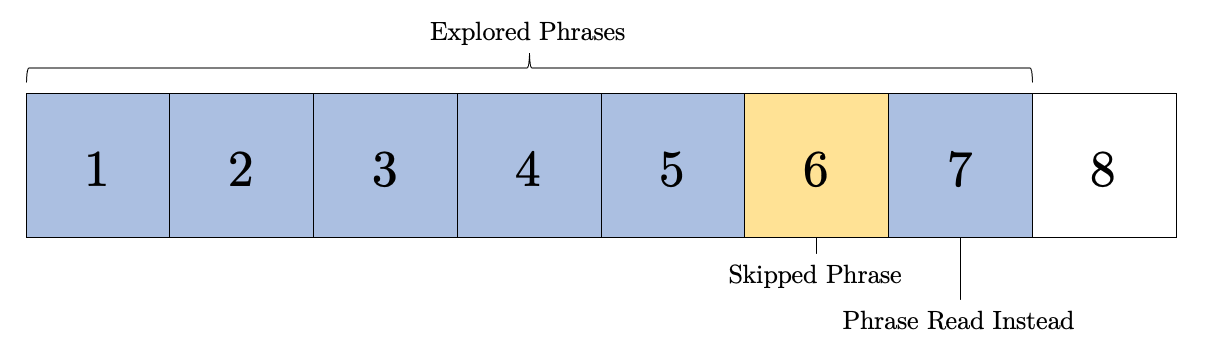
\includegraphics[width=\linewidth]{images/phrase-selection/phrase-skip.png}
    \caption*{Source: Author}
    \label{fig:falealgumacoisa-phrase-skip}
\end{figure}

\subsection{Filtering Criteria}

In addition to the number of phrases per group, the selection process of each phrase must be further detailed. This section specifies such characterizations, requiring the phrases to adhere to some criteria. Such phrase:

\begin{enumerate}
    \item must start with a capital letter and end with a period, so that it is selfcontained;
    \item must not contain more than 110 characters, so that it fits within the breakpoints specification of the recording page;
    \item must be related to the theme chosen, to compound the knowledge of the other spoken phrases in the same theme;
    \item must be a fact, or at least reviewed by one or more individuals, so that there is no spread of misinformation;
    \item must be in Portuguese, since it is a Portuguese corpus;
    \item must not use very uncommon words, to facilitate reading;
    \item must be copyright free, for use in the application.
\end{enumerate}

\subsection{Phrases Source}

To extract phrases with such requirements, the source of phrases must be vast. Fortunately, Wikipedia has a monthly backup dump that contains all pages in text format. The latest version of the Portuguese backup is also available in \url{https://dumps.wikimedia.org/ptwiki/20210120/}, and was generated in 01/20/2021.

This extraction was downloaded using the following command \ref{lst:download}:

\begin{lstlisting} [language=Bash, caption={Download and extraction of the Portuguese Wikipedia latest extraction}, captionpos=t, source={Author}, label={lst:download}]
wget https://dumps.wikimedia.org/ptwiki/20210120/ptwiki-20210120-pages-articles-multistream.xml.bz2 bzip2 -d
ptwiki-20210120-pages-articles-multistream.xml.bz2
\end{lstlisting}

To set a baseline for comparison, the initial extraction (formatted in xml) was filtered to separate phrases (list of strings) from all pages. The definition of a phrase in the context of this work is simple: "string that starts with a capital letter and ends with a period". This extraction yielded 100.000.000.000 phrases distributed in a wide range of pages (1.000.000): places, historical moments, people, concepts, animals, etc.

\subsection{Phrases Filtering}

However, the list still needs further filtering, since many criteria are still not satisfied. The figure \ref{fig:phrase-selection-pyramid} illustrates the process of applying criteria, such as removal of less common words, filtering of themes and finally length limitation.

\begin{figure}[h]
    \centering
    \caption{Filtering process for obtaining phrases for the Fale Alguma Coisa WebApp}
    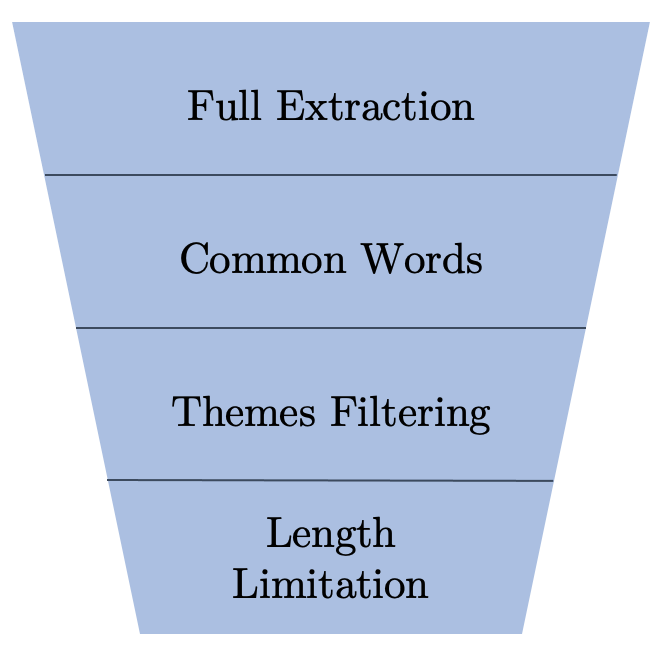
\includegraphics[width=0.5\linewidth]{images/phrase-selection/filtering-pyramid.png}
    \caption*{Source: Author}
    \label{fig:phrase-selection-pyramid}
\end{figure}

The extraction of a list of common words is based on the more frequent words. To identify these words, the script at \url{https://github.com/gabrieltnishimura/cv-sentence-extractor} \footnote{Based on \url{https://github.com/dabinat/cvtools/}, \url{https://github.com/common-voice/cv-sentence-extractor}, and \url{https://github.com/attardi/wikiextractor.git}} was used as follow:

\begin{lstlisting} [language=Bash, caption={Download and extraction of word frequency list}, captionpos=t, source={Author}, label={lst:word-frequency-script}]
# download script
git clone https://github.com/gabrieltnishimura/cv-sentence-extractor
# extraction of phrases
python3 WikiExtractor.py --json ptwiki-latest-pages-articles-multistream.xml
cargo run -- extract -l en -d text/ --no_check >> wiki.pt.all.txt
# creation of frequency list
python3 word_usage.py -i wiki.pt.all.txt >> word_usage.pt.txt
\end{lstlisting}

The result of the script is a file with the tuple \texttt{<word, frequency>}, and one simplified example is available at listing \ref{lst:word-frequency-example}.

\begin{lstlisting} [caption={Word frequency extraction example from the Portuguese Wikipedia (word_usage.pt.txt)}, captionpos=t, source={Author}, label={lst:word-frequency-example}]
de 172609
a 159800
o 135680
e 109532
do 63474
...
volta 1694
exemplo 1685
faz 1680
vai 1673
dentro 1668
...
trabalhavam 49
transações 49
turística 49
unem 49
vela 49
...
op 9
opaco 9
ophelia 9
orbitam 9
orchestra 9
\end{lstlisting}

With the frequency list, it is possible to decide what words are the most common in this extraction. According to Mozilla (\url{https://github.com/common-voice/cv-sentence-extractor}), words with 80-60 repetitions are considered infrequent, and should be removed. Applying this rule, the list is reduced to 90.000.000 phrases.

The next step in filtering is the separation of themes that do not teach a concept. These are places and people. This removal is done by verifying some characteristics in the Wikipedia page metadata, such as latitude or date of birth. After this removal, the extraction yielded 30.000.000 phrases.

Finally, these valid pages with more common words must be filtered by length, to fit inside the phrase box in the user interface. This results into a list of 100.000 phrases, that can be used to populate the application.

\begin{table}[h]
    \centering
    \caption{Phrases Filtering Results of the Portuguese Wikipedia (extracted 01/20/2021)}
    \label{tab:filtering}
    \begin{tabular}{|p{5cm}|p{3cm}|p{3cm}|}
        \hline Step & Pages (Themes) & Phrases \\ \hline
        Full extraction & 1.000.000 & 1.000.000.000 \\ \hline
        Common words & 3.000.000 & 90.000.000 \\ \hline
        Themes filtering & 100.000 & 30.000.000 \\ \hline
        Length limitation & 20.000 & 100.000 \\ \hline
    \end{tabular}
    \caption*{Source: Author}
\end{table}

\subsection{Image Selection}

With the filtering done, a list of themes with the minimum threshold of phrases was generated. According to \ref{uc:20}, themes need an image to be displayed in two pages: the dashboard and the recording page. This section specifies the selection of such images, but since they are going to be used directly in the user interface, they need to be selected with more care. Factors such as resolution, size, format, and license must be taken into consideration.

Each theme was selected using the Pexels, a website for stock photo and videos, distributing images that can be downloaded and used for free. Pexels has a simple license allowing users to download, use without attribution, and edit the media without permission. This would be ideal for the Fale Alguma Coisa app that would display these images.

\subsection{Application Input}

With the filtering and image selection done, the themes can be inputted in the application, so that users view the themes in the dashboard and recording page. According to use case \ref{uc:40}, a REST API will expose the insertion of theme functionality.  

\section{Development}
\label{sec:app-development}

The previous sections in this chapter had detailed explanations of non-technical characteristics of the application. These characteristics help understand the "what" that compromises the voice recording WebApp, detailing functionality and behavior through use cases, navigation semantics and user interface. The development section hereby details the "how", delving into the technical particularities involved when creating this kind of application. The sections below detail three different perspectives on specifying the development: (1) architectural model, and (2) development model.

\subsection{Architecture Model}

In the architecture model, it is necessary to define each component of the system, specifying their responsibility in the business process. The figure \ref{fig:webapp-architecture} illustrates a simple architecture diagram. The citizen scientist will access the application WebApp, which will make requests to the Backend. This backend will in turn translate these requests into a database query, retrieving or altering data.

\begin{figure}[h]
    \centering
    \caption{Architecture diagram for the proposed WebApp}
    \label{fig:webapp-architecture}
    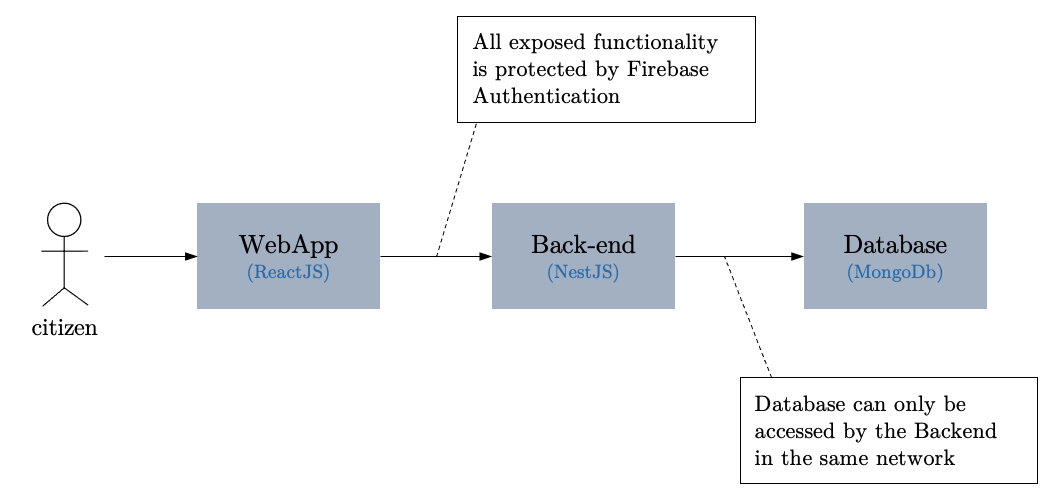
\includegraphics[width=\linewidth]{images/sw-req-spec/architecture.png}
    \caption*{Source: Author}
\end{figure}

These three components are defined below:

\subsubsection{WebApp}

To allow easier access to the voice recording app, a web-based application will be developed. This factor positively influences the capacity of the app to update over time, when compared to an application developed in a native environment. It also enables users over mobile and desktop to access the same application, and although the layout may have to be redesigned, most logic is reused. 

This application performs most of the user interface logic in the web browser, communicating with the Backend to fetch or persist data, for example. This kind of WebApp is called Single Page Application (SPA), and communicates with the Backend primarily using web APIs.

\subsubsection{Backend}

To separate the visual interface of the SPA with the necessary data interactions, it is common to provide such functionality through a Backend. The Backend is a separate component that serves an integration point between the WebApp and the persistence layer (database). It encapsulates many business rules (for example, in the Fale Alguma Coisa Backend, whenever the user records a theme, he receives a set number of points), processing them as requested.

\subsubsection{Database}

To persist voice recordings, user scoring, friend list, etc, it is necessary to provide a database. To allow for further modifications of the data structure defined in the Domain Model in the Appendix (\ref{appendix:srs:domain-model}), a NoSQL database will be chosen.

\subsection{Development Model}

The development model specifies the tools and frameworks selected to execute the implementation. Each selection below will have a respective explanation, albeit simplified. The topics of discussion are presented below.

\subsubsection{Tools Selection}

To develop the application, a selection of tools was made. The table \ref{tab:tools-selection} details the selected tools and explains each choice.

\begin{table}[h]
    \centering
    \caption{Tools Selected to help the development of the Fale Alguma Coisa app.}
    \label{tab:tools-selection}
    \begin{tabular}{|p{5cm}|p{2.5cm}|p{7cm}|}
        \hline Category & Selection & Description \\
        \hline Design & Zeplin & Collaboration tool for sharing layouts \\ 
        \hline Version Control System (VCS) & GitHub & Open-source repository storage \\
        \hline Management & GitHub Projects & Simple task management tool \\
        \hline Continuous Integration (CI) & Circle CI & Automated Pipeline providing testing and building capabilities \\ 
        \hline Continuous Delivery (CD) & Heroku & Platform as a Service to provide the application an cloud environment for testing \\ 
        \hline Integrated Development Environment (IDE) & Visual Studio Code & Simple IDE to develop applications \\ \hline 
    \end{tabular}
    \caption*{Source: Author}
\end{table}

\subsubsection{Frameworks Selection}

Within the wide range of frameworks to develop a web application, back-end, and database, the selection at table \ref{tab:frameworks-selection} was made based on familiarity with the Javascript ecossystem.

\begin{table}[h]
    \centering
    \caption{Frameworks Selected to help the development of the Fale Alguma Coisa app.}
    \label{tab:frameworks-selection}
    \begin{tabular}{|p{5cm}|p{2.5cm}|p{7cm}|}
        \hline Category & Selection & Description \\
        \hline Web & ReactJS & Javascript Web Framework \\ 
        \hline Backend & NestJS & Server side applications with Typescript \\ 
        \hline Database & MongoDB & Document oriented NoSQL \\ 
        \hline Testing & Jest & Testing framework for both WebApp and Backend \\ \hline 
    \end{tabular}
    \caption*{Source: Author}
\end{table}

\subsubsection{Repositories}

The development for this application was mainly made in two repositories:

\begin{itemize}
    \item WebApp: \url{https://github.com/gabrieltnishimura/react-falaalgumacoisa}
    \item Backend: \url{https://github.com/gabrieltnishimura/node-falaalgumacoisa}
\end{itemize}

	\chapter{General Public Submission}
\label{chap:proposal-public-submission}

At the time of this writing, the application is available in the temporary url \url{https://falealgumacoisa.herokuapp.com/}. The application will be published to the url \url{https://falealgumacoisa.pcs.usp.br/}. After, the public will be able to contribute their voices.

	\chapter{Data Analysis}
\label{chap:proposal-data-analysis}

The data analysis will occur during the public submission period, and will end after 1 month of recordings. This analysis will create a first version of the Fale Alguma Coisa Speech Corpus, which will be published in section \ref{sec:proposal-data-publication}. This process will be thoroughly documented, so it may be reproduced afterwards to add more recordings to a more recent version of the corpus.

This data analysis consists in 4 main steps: (1) definition of recording structure, (2) filtering of unusable recordings, (3) association of the user metadata with the recordings, (4) statistical analysis to ensure data quality.

	\chapter{Data Publication}
\label{chap:proposal-data-publication}

After the data analysis this dataset will be published under the CC-BY-4 open-source license. It will be available in the USP dataset repositories.
	\apendices
	\chapter{Software Requirements Specification}
\label{appendix:srs}

\section{Introduction}
\subsection{Purpose}

The purpose of this Requirements Specification is to document the software requirements of Fale Alguma Coisa, a citizen science voice recording app. It should be used by anyone with the intent of understanding what are the capabilities of the system. This document will not focus on how the system will be built, but serves as the basis for the design and implementation. The design is documented within the Design Model in appendix \ref{appendix:design-model}. Details on implementation are documented in the corresponding Software Design Description (SDD) document in the appendix \ref{appendix:software-design-description}.

\subsection{Scope}

\subsubsection{Objectives}

Towards contributing \textbf{nonprofessional scientists}, the Fale Alguma Coisa app should provide an easy gateway for the user to contribute his voice while having fun and learning various science facts and curiosities.

Towards researching \textbf{scientists}, the Fale Alguma Coisa app should provide a database of anonymized voice recordings, for scientists to extract and create speech corpus.

\subsubsection{Outside scope}

However, some elements are outside of the scope of this system. Fale Alguma Coisa should \textbf{not}:
\begin{itemize}
    \item Allow for association of recording data and personal identification data (name, email);
    \item Support internationalization in the WebApp;
    \item Convert audio data into another format
    \item Support offline recording
\end{itemize}

\subsubsection{Artifacts}

This document identifies the following artifacts to be produced:

\begin{itemize}
    \item Context
    \item Domain Model
    \item Use Case Requirements (Actors, Diagrams, Specifications)
    \item Activity Diagrams
    \item Non-Functional Requirements
    \item Interface Requirements
    \item WebApp for user recordings
    \item Backend with database
\end{itemize}

\subsection{Overview of Document}

This overview provides a summary of the contents of each section of this document.

\begin{itemize}
    \item Introduction
    \item System Overview
    \item Domain Model
    \item Requirements
\end{itemize}

\subsection{References}

\begin{itemize}
    \item Based on: \cite{naoufel2014requirements}
    \item Supporting literature: \cite{pressman2014software}
\end{itemize}

\section{System Overview}

The System Overview section presents the system context and design, and also discusses the background of the Fale Alguma Coisa project.

\subsection{Name}

This system is called "Fale Alguma Coisa". This is a phrase in brazillian portuguese to order someone to "say something". It is also common to hear "fala alguma coisa", but this was changed to remove the alliteration effect, providing easier spelling.

\subsection{System Context}

This system is originated from the need of recording anonymized user voices throughout the use of gamification and citizen science.

\subsection{General Constraints}

This system is mainly impacted by constraints in data privacy. Recordings should never be associated with the users personal data (such as email), but should have metadata to aid in corpus construction, such as age interval, gender, and dialect.

\subsection{Assumptions and Dependencies}

The system heavily depends on the phrases that will be spoken. Therefore it is necessary to provide this application with a comprehensive list of phrases before the application general publication.

\section{Analysis Model}

To accurately describe the software requirements of a project, it is important to understand the requirements from many different perspectives. The analysis model proposed by \cite{pressman2014software} encompasses four different modeling elements (perspectives) that can be used to provide the most effective bridge to software design. They are listed in the subsections below as (1) scenario based models, (2) class-based elements model, (3) behavioral elements, and (4) flow-oriented elements. The analysis can lead to the derivation of one or more of these modeling elements, since one model may not completely describe certain functionalities of the app.

\subsection{Scenario-based models}

This model depicts how the user interacts with the system and the specific sequence of activities that occur as the software is used. One common implementation for this specification is through use cases. To provide scenario-model completeness, the following sections will describe every use case mapped to the WebApp. They are, however, not extensive to the functionality of the application, some use cases are complemented by the models cited above. Each of the use cases are categorized by feature. Furthermore, each feature is described in the table \ref{tab:falealgumacoisa-features}.

\begin{table}[h]
    \centering
    \caption{WebApp Fale Alguma Coisa Features}
    \label{tab:falealgumacoisa-features}
    \begin{tabular}{|p{3cm}|p{10cm}|}
        \hline Epic & Description \\
        \hline Points & Represents the user stories affecting the homepage, such as the splash screen, call to action button, terms of service, etc. \\
        \hline Recording & Represents the most important feature in the application, as the citizen will use it to record his voice. It also provides supporting features, such as skipping phrases and resuming the recording session.\\ 
        \hline Dashboard & Lists all user stories related to the dashboard page, such as where the user will be able to choose themes to record, open the menu, check his level, etc. \\
        \hline Gamification & Details the engagement component of the application. Elements such as leaderboards, points and levels are described. They add a sense of progress to the user experience. \\
        \hline Social & To allow social interaction with other users, this feature lists social features to be added to the application. \\
        \hline Login and Registration & The application should provide user authentication to enable data management and progress saving. \\
        \hline
    \end{tabular}
    \caption*{Source: Author}
\end{table}

\begin{table}[h]
\caption{Use cases categorized to the home epic for the Fale Alguma Coisa WebApp}
\label{tab:falealgumacoisa-home-epic}
\centering
\begin{tabular}{|p{2cm}|p{1cm}|p{10cm}|}
\hline
Epic & Code & User Story \\ \hline
\multirow{5}{*}{Home} 
    & US01 & I, as an unregistered citizen, would like to view an animated introductory screen in the application, so that I feel more inside a native app. \\ \cline{2-3} 
    & US02 & I, as an unregistered citizen, would like to know more about Fale Alguma Coisa from a explanatory text in the homepage, so that I understand more about the project. \\ \cline{2-3} 
    & US03 & I, as a registered citizen, would like to easily go from the homepage to the sign-in page, so that I can login to my account. \\ \cline{2-3} 
    & US04 & I, as an unregistered citizen, would like to click a call to action button to go from the homepage to the recording page from the homepage, so that I can contribute my voice. \\ \cline{2-3} 
    & US05 & I, as an unregistered citizen, would like to read the terms of service and privacy policy of Fale Alguma Coisa, so that I understand better what the service has to offer and what kind of data will be recorded. \\ \hline
\end{tabular}
\caption*{Source: Author}
\end{table}

\begin{table}[h]
\caption{User Stories categorized to the recording epic for the Fale Alguma Coisa WebApp}
\label{tab:falealgumacoisa-recording-epic}
\centering
\begin{tabular}{|p{2cm}|p{1cm}|p{10cm}|}
\hline
Epic & Code & User Story \\ \hline
\multirow{9}{*}{Recording} 
    & US10 & I, as an unregistered citizen, would like to view and accept the terms of service before recording, so that I understand how my data is being used. \\ \cline{2-3} 
    & US11 & I, as an unregistered citizen, would like to properly configure my microphone before recording, so that I can record without interruption. \\ \cline{2-3} 
    & US12 & I, as a citizen, would like to read science phrases with definitions and curiosities, so that I learn about subjects as I am contributing. \\ \cline{2-3} 
    & US13 & I, as a citizen, would like to read phrases grouped by theme, so that I can learn more from each subject as I am contributing. \\ \cline{2-3} 
    & US14 & I, as a citizen, would like to read a tutorial explaining how to record, so that I learn how to properly record phrases. \\ \cline{2-3} 
    & US15 & I, as a citizen, would like to see animations on each step of the recording (enter the page, start the recording, stop the recording), so that I feel more engaged with the application. \\ \cline{2-3} 
    & US16 & I, as a citizen, would like to skip a phrase when I (1) do not know how to pronounce, or (2) find a foreign word, or (3) another specified reason, so that I only speak the correct phrases. \\ \cline{2-3} 
    & US17 & I, as a unregistered citizen, would like to stop this recording session by returning home when clicking the logo and confirming the exit, so that I can resume it afterwards. \\ \cline{2-3} 
    & US18 & I, as a registered citizen, would like to return to the dashboard after clicking the logo and confirming the exit, so that I can resume it afterwards. \\ \hline
\end{tabular}
\caption*{Source: Author}
\end{table}

\begin{table}[h]
\caption{User Stories categorized to the dashboard epic for the Fale Alguma Coisa WebApp}
\label{tab:falealgumacoisa-dashboard-epic}
\centering
\begin{tabular}{|p{2cm}|p{1cm}|p{10cm}|}
\hline
Epic & Code & User Story \\ \hline
\multirow{6}{*}{Dashboard} 
    & US20 & I, as an unregistered citizen, would like to easily register my data through a button click, so that I can enjoy all features of the logged area. \\ \cline{2-3} 
    & US21 & I, as a registered citizen, would like to see my actions in a dashboard after logging in, so that I can better contribute to the project. \\ \cline{2-3} 
    & US22 & I, as a registered citizen, would like to see a list of recommended themes to speak, so that I can choose one from the list. \\ \cline{2-3} 
    & US23 & I, as a registered citizen, would like to view my progress level, so that I know how far have I progressed in my contributions. \\ \cline{2-3} 
    & US24 & I, as a registered citizen, would like to open the menu, so that I know which are my possible actions in the app. \\ \cline{2-3} 
    & US25 & I, as a registered citizen, would like to check notifications, so that I understand what happened while I was gone. \\ \hline
\end{tabular}
\caption*{Source: Author}
\end{table}

\begin{table}[h]
\caption{User Stories categorized to the gamification epic for the Fale Alguma Coisa WebApp}
\label{tab:falealgumacoisa-gamification-epic}
\centering
\begin{tabular}{|p{2.5cm}|p{1cm}|p{10cm}|}
\hline
Epic & Code & User Story \\ \hline
\multirow{6}{*}{Gamification}
    & US30 & I, as a registered citizen, would like to get 100 points when I record my first phrase, so that I can engage better in the application. \\ \cline{2-3} 
    & US31 & I, as a registered citizen, would like to get 400 points when I record my first theme, so that I can engage better in the application. \\ \cline{2-3} 
    & US32 & I, as a registered citizen, would like to get 300 points when I record subsequent themes, so that I can engage better in the application. \\ \cline{2-3} 
    & US33 & I, as a registered citizen, would like to get 500 points when I register my data, so that I can better engage with the application. \\ \cline{2-3} 
    & US34 & I, as a registered citizen, would like to measure my points through a level, so that I can more easily compare myself with other users. \\ \hline
\end{tabular}
\caption*{Source: Author}
\end{table}

\begin{table}[h]
\caption{User Stories categorized to the social epic for the Fale Alguma Coisa WebApp}
\label{tab:falealgumacoisa-social-epic}
\centering
\begin{tabular}{|p{2cm}|p{1cm}|p{10cm}|}
\hline
Epic & Code & User Story \\ \hline
\multirow{6}{*}{Social}
    & US40 & I, as a registered citizen, would like to know who are the top contributors in the space and where am I in the list, so that I can compete against them. \\ \cline{2-3} 
    & US41 & I, as a registered citizen, would like to know where my friends are in a more customized leaderboard, so that I can compete against them. \\ \cline{2-3} 
    & US42 & I, as a registered citizen, would like to add a friend, so that I can check them in the friends leaderboard afterwards. \\ \cline{2-3} 
    & US43 & I, as a registered citizen, would like to check notifications, so that I can know what happened when I was away. \\ \cline{2-3} 
    & US44 & I, as a registered citizen, would like to know when someone added me through notifications, so that I can add them back later. \\ \cline{2-3} 
    & US45 & I, as a registered citizen, would like to refer friends to the application, so that I can play with them. \\ \hline
\end{tabular}
\caption*{Source: Author}
\end{table}

\begin{table}[h]
\caption{User Stories categorized to the login and registration epic for the Fale Alguma Coisa WebApp}
\label{tab:falealgumacoisa-login-and-registration-epic}
\centering
\begin{tabular}{|p{3cm}|p{1cm}|p{10cm}|}
\hline
Epic & Code & User Story \\ \hline
\multirow{4}{*}{\shortstack[l]{Login and \\ Registration}} 
    & US50 & I, as an unregistered citizen, would like to login (using social login - Facebook / Google) on the app, so that I can login later and save my progress. \\ \cline{2-3} 
    & US51 & I, as a unregistered citizen, would like to register my anonymous data on my first login, so that I can provide better metadata to my recordings afterwards. \\ \cline{2-3} 
    & US52 & I, as a registered citizen, would like to update my account data, so that I can provide accurate metadata on the recordings. \\ \cline{2-3} 
    & US53 & I, as a registered citizen, would like to remove my account data (and my recordings, if necessary), so that I can remove my metadata from this application. \\ \hline
\end{tabular}
\caption*{Source: Author}
\end{table}

\subsubsection{Usability}

The usability epic details user stories related to the user experience with the app.

\begin{itemize}
    \item I, as a citizen, would like to contribute my voice using my mobile devices and desktop computer.
\end{itemize}

\subsection{Class models}

\subsection{Behavioral models}

\subsection{Flow models}

 

	\anexos
	\chapter{Ten principles of citizen science}
\label{app:ten-principles}

\begin{itemize}
    \item Citizen science projects actively involve citizens in scientific endeavour that generates new knowledge or understanding. 
    \subitem Citizens may act as contributors, collaborators or as project leaders and have a meaningful role in the project.
    \item Citizen science projects have a genuine science outcome. For example, answering a research question or informing conservation action, management decisions or environmental policy.
    \item Both the professional scientists and the citizen scientists benefit from taking part. Benefits may include the publication of research outputs, learning opportunities, personal enjoyment, social benefits, satisfaction through contributing to scientific evidence, for example, to address local, national and international issues, and through that, the potential to influence policy.
    \item Citizen scientists may, if they wish, participate in multiple stages of the scientific process. This may include developing the research question, designing the method, gathering and analysing data, and communicating the results.
    \item Citizen scientists receive feedback from the project. For example, how their data are being used and what the research, policy or societal outcomes are.
    \item Citizen science is considered a research approach like any other, with limitations and biases that should be considered and controlled for. However unlike traditional research approaches, citizen science provides opportunity for greater public engagement and democratisation of science.
    \item Citizen science project data and metadata are made publicly available and where possible, results are published in an open-access format. Data sharing may occur during or after the project, unless there are security or privacy concerns that prevent this.
    \item Citizen scientists are acknowledged in project results and publications.
    \item Citizen science programmes are evaluated for their scientific output, data quality, participant experience and wider societal or policy impact.
    \item The leaders of citizen science projects take into consideration legal and ethical issues surrounding copyright, intellectual property, data-sharing agreements, confidentiality, attribution and the environmental impact of any activities.
\end{itemize}
% 	% ----------------------------------------------------------


% 	% ----------------------------------------------------------
% 	% Prepara pdf para iniciar o bookmark na raiz
% 	% ----------------------------------------------------------
	\phantompart

% 	% ----------------------------------------------------------
% 	% Conclusão
% 	% ----------------------------------------------------------
% 	%\include{conclusao}
% 	% ----------------------------------------------------------

% 	% ----------------------------------------------------------
% 	% ELEMENTOS PÓS-TEXTUAIS
% 	% ----------------------------------------------------------
	\postextual
% 	% ----------------------------------------------------------

% 	% ----------------------------------------------------------
% 	% Referências bibliográficas
% 	% ----------------------------------------------------------
	\bibliography{referencias}

\end{document}